\documentclass[11pt,a4paper,twoside,openany]{book}
\usepackage{amsmath,amssymb}
\usepackage[sc]{mathpazo}
\usepackage[no-math]{fontspec}
\setmainfont{texgyrepagella}[Extension=.otf,UprightFont=*-regular,BoldFont=*-bold,ItalicFont=*-italic,BoldItalicFont=*-bolditalic]
\setsansfont{DejaVu Sans}[Scale=0.88]
\setmonofont{DejaVu Sans Mono}[Scale=0.82]
\usepackage{polyglossia}
\setdefaultlanguage{french}
\usepackage[a4paper,top=2.6cm,bottom=2.6cm,inner=2.7cm,outer=2.3cm,headheight=14pt]{geometry}
\usepackage{xcolor}
\definecolor{bleu}{HTML}{1F4E79}
\definecolor{bleuclair}{HTML}{EEF3F8}
\definecolor{orange}{HTML}{C55A11}
\definecolor{orangeclair}{HTML}{FDF1E7}
\definecolor{vert}{HTML}{2C7C3C}
\definecolor{vertclair}{HTML}{EDF6EE}
\definecolor{rouge}{HTML}{A61B1B}
\definecolor{rougeclair}{HTML}{FBECEC}
\definecolor{gris}{HTML}{555555}
\usepackage{graphicx}
\graphicspath{{../figures/}}
\usepackage{booktabs,longtable,tabularx,array,multirow}
\usepackage{caption}
\usepackage{adjustbox}
\newcommand{\tabfit}[1]{\adjustbox{max width=\linewidth}{\input{#1}}}
\captionsetup{font={small},labelfont={bf,color=bleu},format=hang}
\usepackage[most]{tcolorbox}
\usepackage{enumitem}
\setlist{itemsep=2pt,topsep=4pt}
\usepackage{fancyhdr}
\pagestyle{fancy}
\fancyhf{}
\fancyhead[LE]{\small\sffamily\color{gris}\leftmark}
\fancyhead[RO]{\small\sffamily\color{gris}\rightmark}
\fancyfoot[C]{\small\sffamily\thepage}
\renewcommand{\headrulewidth}{0.3pt}
\usepackage{titlesec}
\titleformat{\chapter}[display]{\sffamily\bfseries\color{bleu}}{\large\MakeUppercase{\chaptertitlename}\ \thechapter}{4pt}{\LARGE}
\titleformat{\section}{\sffamily\bfseries\Large\color{bleu}}{\thesection}{0.8em}{}
\titleformat{\subsection}{\sffamily\bfseries\large\color{bleu}}{\thesubsection}{0.8em}{}
\titleformat{\subsubsection}{\sffamily\bfseries\normalsize\color{bleu!80!black}}{\thesubsubsection}{0.6em}{}
\titleformat{\part}[display]{\centering\sffamily\bfseries\color{bleu}}{\Large\MakeUppercase{\partname}\ \thepart}{12pt}{\Huge}
\setcounter{secnumdepth}{3}
\setcounter{tocdepth}{2}
\usepackage{siunitx}
\sisetup{output-decimal-marker={,},group-separator={\,},group-minimum-digits=4}
\usepackage[hidelinks,bookmarksnumbered]{hyperref}
\hypersetup{pdftitle={L'économie française au banc d'essai : documentation, simulations et stratégies},pdfauthor={Projet Présidentielle}}
\usepackage{xurl}

% Encadrés
\newtcolorbox{encadre}[1]{enhanced,breakable,colback=bleuclair,colframe=bleu,fonttitle=\sffamily\bfseries\small,title={#1},boxrule=0.5pt,arc=1mm,left=6pt,right=6pt,top=4pt,bottom=4pt,fontupper=\small}
\newtcolorbox{hypothese}[1][Hypothèses retenues]{enhanced,breakable,colback=orangeclair,colframe=orange,fonttitle=\sffamily\bfseries\small,title={#1},boxrule=0.5pt,arc=1mm,left=6pt,right=6pt,top=4pt,bottom=4pt,fontupper=\small}
\newtcolorbox{limites}[1][Limites]{enhanced,breakable,colback=rougeclair,colframe=rouge,fonttitle=\sffamily\bfseries\small,title={#1},boxrule=0.5pt,arc=1mm,left=6pt,right=6pt,top=4pt,bottom=4pt,fontupper=\small}
\newtcolorbox{resultat}[1][À retenir]{enhanced,breakable,colback=vertclair,colframe=vert,fonttitle=\sffamily\bfseries\small,title={#1},boxrule=0.5pt,arc=1mm,left=6pt,right=6pt,top=4pt,bottom=4pt,fontupper=\small}
\newtcolorbox{exemple}[1][Exemple numérique]{enhanced,breakable,colback=white,colframe=gris,fonttitle=\sffamily\bfseries\small,title={#1},boxrule=0.4pt,arc=1mm,left=6pt,right=6pt,top=4pt,bottom=4pt,fontupper=\small}

% Niveaux de preuve
\newcommand{\preuve}[1]{\textsf{\small\bfseries\color{bleu}[#1]}}
\newcommand{\fiab}[1]{\textsf{\footnotesize\bfseries\colorbox{bleuclair}{\color{bleu}#1}}}
\newcommand{\src}[1]{{\small\color{gris}[#1]}}
\newcommand{\code}[1]{\texttt{\small #1}}
\newcommand{\md}{\,Md€}
\newcommand{\pt}{\,pt}
\renewcommand{\arraystretch}{1.15}
\newcolumntype{R}{>{\raggedleft\arraybackslash}X}
\newcolumntype{L}{>{\raggedright\arraybackslash}X}
\newcolumntype{C}{>{\centering\arraybackslash}X}
\setlength{\parskip}{3pt}
\raggedbottom
\emergencystretch=3em
\renewcommand{\code}[1]{\texttt{\small\hyphenchar\font=`\-\relax #1}}


\begin{document}
\frontmatter
\begin{titlepage}
\thispagestyle{empty}
\sffamily
\vspace*{1.5cm}
{\color{orange}\large\bfseries RAPPORT SCIENTIFIQUE, PÉDAGOGIQUE ET PROSPECTIF\par}
\vspace{0.8cm}
{\color{bleu}\fontsize{28}{34}\selectfont\bfseries L'économie française\\[2pt] au banc d'essai\par}
\vspace{0.5cm}
{\color{bleu}\Large Ce que montre un modèle ouvert de la France :\\ mécanismes, expériences, stratégies de redressement\par}
\vspace{0.8cm}
{\color{bleu}\rule{\linewidth}{1.2pt}}
\vspace{0.6cm}

{\large\color{gris}Projet « Présidentielle » — modèle économique et social de la France, version 0.6\par}
\vspace{1.2cm}
\renewcommand{\arraystretch}{1.5}
\begin{tabular}{@{}>{\bfseries\color{bleu}}p{4cm}p{10.5cm}@{}}
Date & 18 novembre 2026 \\
Version du modèle & 0.6 (code et résultats : dépôt GitHub du projet, dossier \texttt{rapport/}) \\
Données & Exclusivement ouvertes : Insee, Eurostat, DGFiP, Drees, Banque de France, FMI, COR, douanes, SDES \\
Statut & Document de travail scientifique. Les résultats sont conditionnels aux hypothèses du modèle, qui sont toutes exposées. Ils ne constituent ni une prévision, ni une recommandation politique. \\
\end{tabular}
\vfill
{\small\color{gris}Rédaction et calculs : Claude (Anthropic), à la demande et sous la direction du porteur du projet. Toutes les simulations citées ont été exécutées avec le code du dépôt ; les fichiers de résultats sont fournis avec ce rapport.\par}
\end{titlepage}

\tableofcontents
\chapter*{Avant-propos et mode d'emploi}
\addcontentsline{toc}{chapter}{Avant-propos et mode d'emploi}
\markboth{Avant-propos}{Avant-propos}

Ce rapport poursuit trois objectifs : \textbf{documenter} intégralement le modèle économique et social de la France
construit dans le projet « Présidentielle » ; l'\textbf{utiliser} pour comprendre, par des expériences chiffrées, comment
les politiques publiques se propagent dans l'économie et la société ; en déduire des \textbf{stratégies de redressement}
et en mesurer les arbitrages. Il s'adresse à deux lecteurs à la fois : le lecteur sans formation économique, pour qui
des encadrés pédagogiques et un glossaire (annexe~\ref{ann:glossaire}) expliquent les notions ; l'économiste, qui
trouvera les équations telles qu'elles sont codées, les coefficients estimés avec leurs écarts-types, les sources et
les tests, de quoi critiquer, vérifier et reproduire chaque résultat.

\paragraph{Ce que ce rapport n'est pas.} Ce n'est ni une prévision, ni un programme politique. Toutes les simulations
comparent deux avenirs hypothétiques (avec et sans une mesure) et dépendent d'hypothèses exposées à chaque étape. Le
modèle est un outil de raisonnement chiffré : il rend explicites des chaînes de causalité et en donne des ordres de
grandeur. Il ne démontre pas qu'une mesure « marche » : il montre ce qu'elle produit \emph{si} les comportements du passé
restent valables et \emph{si} les hypothèses retenues sont justes.

\paragraph{Règles suivies.}
\begin{itemize}
\item Toutes les données sont ouvertes ; les sources sont citées au niveau des affirmations.
\item Chaque paramètre a un niveau de preuve (relation comptable, donnée observée, estimé, calibré, transposé de la
littérature, hypothèse) ; chaque résultat un degré de robustesse (\fiab{robuste}, \fiab{plutôt robuste}, \fiab{fragile},
\fiab{non établi}).
\item Une corrélation passée n'est jamais présentée comme un effet causal établi : les coefficients estimés sont des
régularités historiques, dont la validité pour des réformes de grande ampleur n'est pas garantie.
\item Les résultats du modèle (parties I à III) sont séparés des recommandations (partie IV), elles-mêmes conditionnelles
aux choix de pondération entre objectifs, qui sont des choix politiques.
\item Toutes les mesures passent par les mêmes équations, quelle que soit leur origine politique.
\item Tous les chiffres proviennent de simulations réellement exécutées avec le code du dépôt ; les fichiers de résultats
sont fournis.
\end{itemize}

\paragraph{Plan.} La \textbf{partie I} décrit l'architecture du modèle (chapitre 1), chacun de ses sous-modèles avec ses
équations, sa calibration et ses limites (chapitre 2), puis en fait l'audit (chapitre 3). La \textbf{partie II} présente
la situation de référence comparée aux statistiques (chapitre 4), huit expériences qui isolent les mécanismes
(chapitre 5) et des expériences complémentaires sur les interactions (chapitre 6). La \textbf{partie III} recherche des
programmes de redressement par optimisation et les soumet à des tests de robustesse (chapitre 7). La \textbf{partie IV}
répond aux huit questions de la mission et propose un programme hiérarchisé (chapitre 8).

\section*{Résumé des principaux enseignements}

\begin{enumerate}
\item \textbf{La trajectoire « sans mesure » n'est pas soutenable.} Avec un taux d'intérêt de marché de 4,9~\% et une
croissance faible (1,1 à 1,2~\% par an jusqu'en 2032, moins ensuite), le déficit public passerait de 5,1~\% du PIB en 2025 à
9~\% en 2032 et la dette de 116 à 142~\% du PIB. La charge d'intérêts en est le premier moteur (de 2,5 à 5,1 points de PIB),
devant le vieillissement. \fiab{robuste} pour le sens, \fiab{fragile} pour les niveaux après 2035.
\item \textbf{Toute consolidation coûte de l'activité à court terme, mais pas autant selon l'instrument.} Par point de
déficit réduit, une économie sur la production publique (fonctionnement, emplois) coûte environ 2~\% de PIB la première
année ; une hausse de TVA, une économie sur les transferts ou une hausse d'impôt sur le patrimoine, 0,3 à 0,7~\%. Les
effets sur l'activité s'estompent en cinq à dix ans ; les gains sur la dette s'accumulent. \fiab{plutôt robuste}.
\item \textbf{Une hausse d'impôt rapporte d'un quart à un tiers de moins que son rendement statique} la première année,
à cause de l'activité perdue ; aucune hausse d'impôt testée ne réduit les recettes, sauf la tranche supérieure de l'IR si
les contribuables aisés réagissent fortement. \fiab{robuste} pour le signe.
\item \textbf{Les mesures qui réduisent le plus la pauvreté par euro sont des prestations ciblées} (prime d'activité, RSA,
minimum vieillesse). Elles soutiennent l'activité à court terme. Les impôts sur la consommation (TVA, taxe carbone) sont
ceux qui pèsent le plus sur les ménages modestes. \fiab{plutôt robuste} (effets statiques).
\item \textbf{Une hausse générale des salaires ne crée ni ne détruit beaucoup d'activité} : elle redistribue vers les
salariés en emploi, au détriment des revenus fixes et, à moyen terme, de l'emploi. Elle n'augmente pas la pauvreté par
effet de seuil (le revenu disponible croît toujours avec le salaire), mais les taux marginaux effectifs atteignent 55 à
82~\% entre 1 et 2 SMIC. \fiab{plutôt robuste}.
\item \textbf{Seul l'investissement public a, parmi les dépenses, un effet durable sur la production} dans le modèle ;
le report de l'âge de départ est le levier de production le plus puissant à long terme, mais il augmente d'abord le
chômage et ses effets dépendent d'une hypothèse de bouclage non estimée. \fiab{fragile}.
\item \textbf{Les mesures interagissent} : relocalisation industrielle et droits de douane se neutralisent (la riposte et
la hausse des coûts annulent le bénéfice), alors que l'investissement public et le report de l'âge se complètent.
\item \textbf{Aucun programme testé ne stabilise la dette si les taux restent proches de 5~\%.} L'effort nécessaire
(environ 6 points de PIB) dépasse ce que les leviers disponibles peuvent apporter sans récession majeure : un effort
maximal (scénario D) coûte deux années de récession et 6~\% de pouvoir d'achat durablement. La soutenabilité dépend
d'abord des taux d'intérêt et de la croissance.
\item \textbf{Le programme recommandé} (chapitre~\ref{ch:synthese}) combine une consolidation par les instruments les
moins coûteux en activité, une protection ciblée des ménages modestes, l'investissement public et un report progressif
de l'âge de départ à 65 ans. Il réduit le déficit, la pauvreté et la dette par rapport à la référence et augmente la
production à long terme, sans la stabiliser à lui seul : c'est un socle, pas une solution complète.
\item \textbf{Les principales faiblesses du modèle} sont l'absence d'estimation du bouclage de moyen terme, une
représentation de l'offre (productivité, démographie) qui donne des résultats paradoxaux pour les chocs d'offre,
l'absence de bilans financiers et d'anticipations, des dépenses publiques indistinctes, et une microsimulation statique
qui représente mal le haut de la distribution (chapitre~\ref{ch:audit}).
\end{enumerate}


\mainmatter
\part{Le modèle : architecture, équations, calibration}
\chapter{Architecture générale du modèle}
\label{ch:architecture}

\section{Ce que le modèle représente}

Le modèle est une représentation chiffrée de l'économie française, construite pour répondre à une question précise :
\emph{si l'on modifie un impôt, une dépense, une prestation ou une règle, que se passe-t-il pour l'activité, l'emploi,
les prix, les revenus des ménages, les finances publiques et la répartition des niveaux de vie, et à quel horizon ?}
Il ne cherche pas à prévoir l'avenir : il compare deux avenirs possibles, l'un sans la mesure (la \emph{référence}),
l'autre avec. C'est ce que les économistes appellent une \emph{variante}.

Il appartient à la famille des \emph{modèles macro-économétriques semi-structurels} utilisés par l'administration
française (Mésange à l'Insee et à la direction générale du Trésor, FR-BDF à la Banque de France), auxquels il emprunte
la logique : des comportements estimés sur l'histoire (consommer, investir, embaucher, fixer les prix et les salaires,
importer, exporter), insérés dans une comptabilité nationale cohérente qui garantit que chaque euro dépensé par un agent
est reçu par un autre. Il s'en distingue par trois choix :
\begin{enumerate}
  \item il est entièrement construit sur des \textbf{données ouvertes} et son code est public ;
  \item il est relié à une \textbf{microsimulation des ménages} (OpenFisca-France appliqué à un échantillon de ménages
  réels du recensement), qui calcule impôts et prestations ménage par ménage et permet de mesurer la pauvreté et les
  inégalités ;
  \item il décrit l'appareil productif en \textbf{64 produits et 25 branches marchandes}, ce qui permet de suivre la
  propagation d'un choc d'énergie ou d'une politique industrielle d'une branche à l'autre.
\end{enumerate}

\begin{encadre}{Encadré 1.1 — Qu'est-ce qu'un modèle, et que peut-on en attendre ?}
Un modèle est un ensemble d'équations qui relient des grandeurs économiques entre elles. Certaines équations sont des
\textbf{identités comptables}, vraies par définition : le PIB est égal à la somme des valeurs ajoutées, la dette de fin
d'année est égale à la dette de début d'année plus le déficit. D'autres sont des \textbf{équations de comportement} : elles
décrivent comment, \emph{en moyenne dans le passé}, les ménages ont ajusté leur consommation à leur revenu, ou les
entreprises leurs embauches à leur production. Ces relations sont estimées statistiquement ; elles comportent une marge
d'erreur, et rien ne garantit qu'elles resteront valables si l'on change profondément les règles du jeu (c'est la
« critique de Lucas »). Enfin, certaines relations sont des \textbf{hypothèses} faute de données : le modèle les
signale comme telles.

Un modèle est donc un instrument de \emph{raisonnement chiffré} : il rend explicites des chaînes de causalité et en
donne des ordres de grandeur. Il ne remplace ni l'évaluation après coup des politiques, ni le débat sur les choix
de société.
\end{encadre}

\section{Les acteurs et leurs échanges}

La figure~\ref{fig:architecture} présente les grands acteurs (au sens de la comptabilité nationale : les \emph{secteurs
institutionnels}) et les flux qui les relient.

\begin{figure}[htbp]
\centering
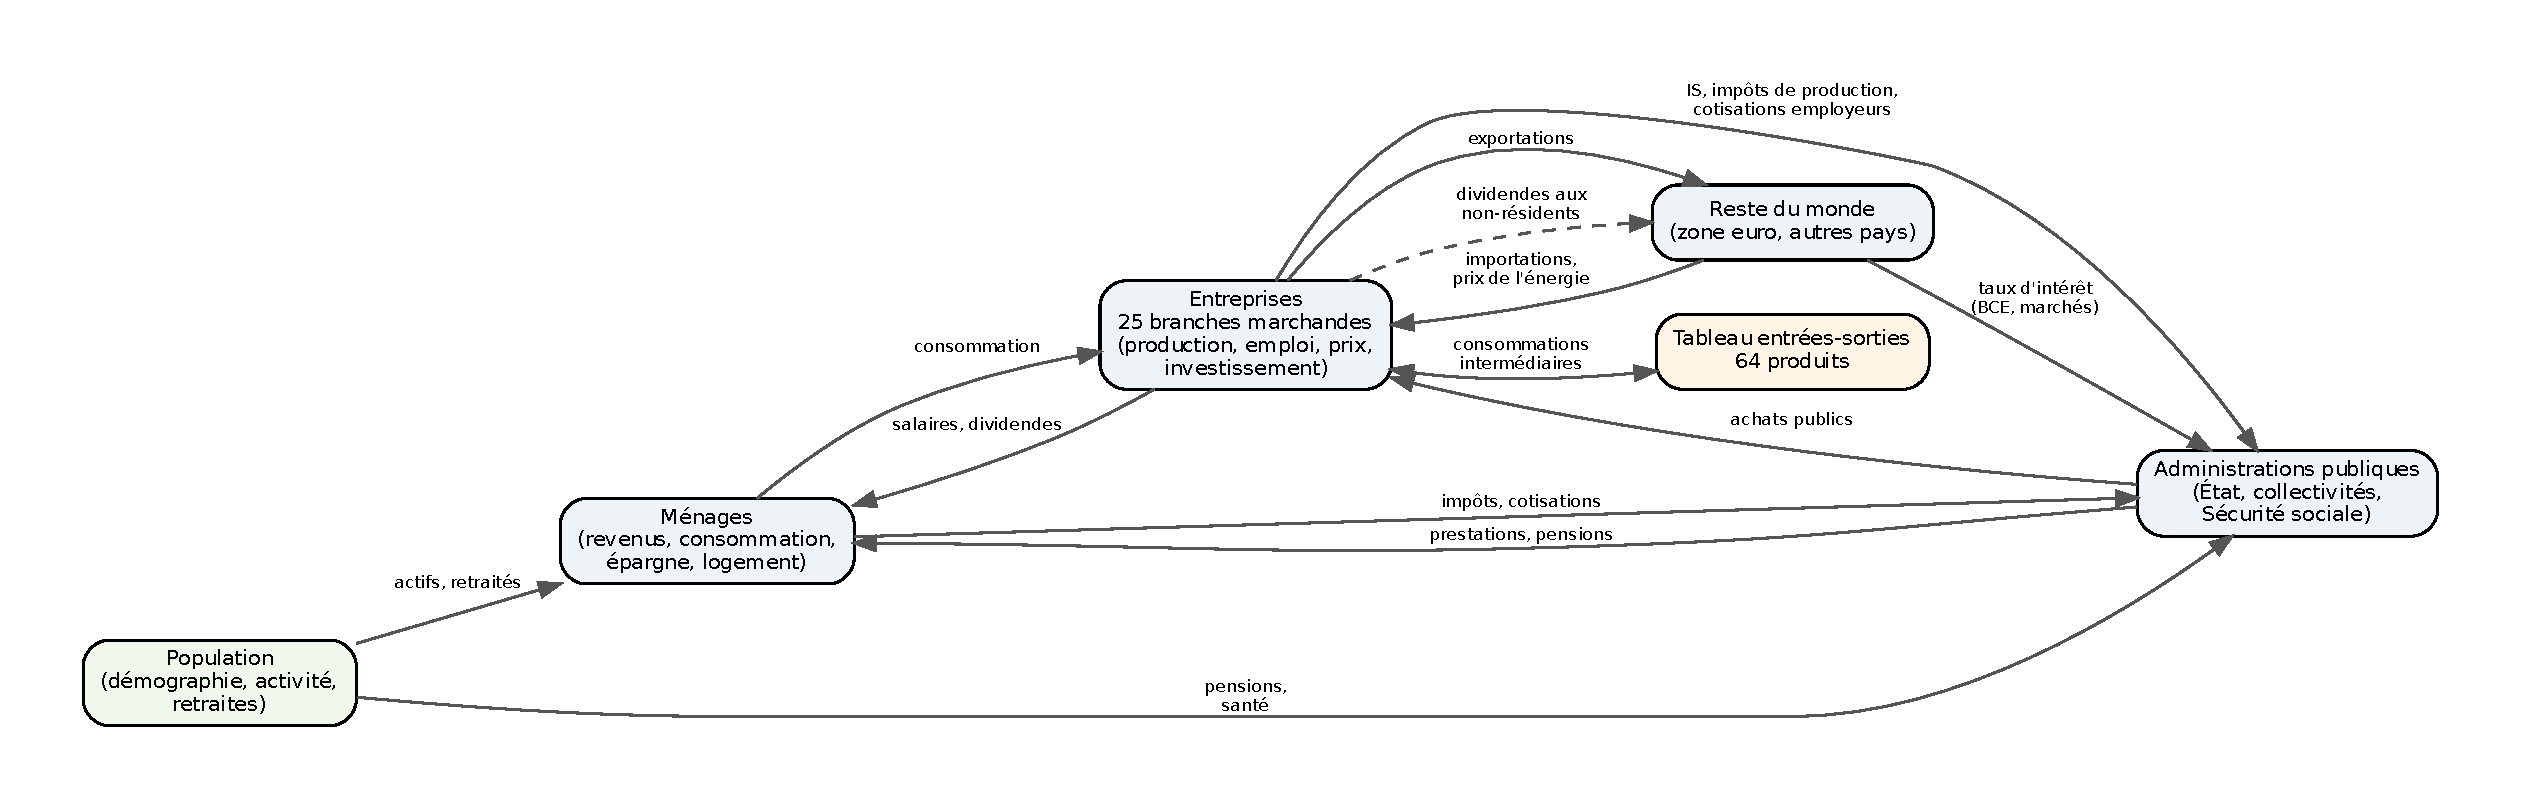
\includegraphics[width=\linewidth]{architecture.pdf}
\caption{Architecture du modèle : secteurs institutionnels et principaux flux. Les flèches pleines sont des flux
monétaires représentés par des équations ; la flèche pointillée (dividendes versés aux non-résidents) n'est active que
pour les mesures qui modifient les profits des entreprises. Le tableau entrées-sorties décrit les échanges entre
produits.}
\label{fig:architecture}
\end{figure}

\begin{description}[style=nextline,leftmargin=1.2em]
\item[Les ménages] perçoivent des salaires, des revenus d'indépendants, des revenus du patrimoine (intérêts,
dividendes, loyers) et des prestations sociales (pensions, allocations, minima sociaux) ; ils paient des impôts
(impôt sur le revenu, CSG) et des cotisations. Ce qui reste est leur \emph{revenu disponible brut} (RDB). Ils en
consomment la plus grande partie, investissent dans le logement et épargnent le reste.
\item[Les entreprises] sont décrites par 25 branches marchandes (agriculture, 15 branches industrielles, énergie,
construction, commerce, transport, hébergement-restauration, information-communication, finance, services aux
entreprises, autres services). Chaque branche produit, emploie, fixe ses prix, investit. La production non marchande
(administration, enseignement, santé publique) et l'immobilier forment une branche à part, dont le volume suit la
dépense publique.
\item[Les administrations publiques] (État, collectivités locales, sécurité sociale, organismes sociaux) prélèvent
impôts et cotisations, versent rémunérations, achats, prestations et intérêts, et s'endettent quand les dépenses
excèdent les recettes. Le modèle ne distingue pas les sous-secteurs : les organismes de sécurité sociale (retraites,
assurance maladie, chômage) sont consolidés avec l'État et les collectivités, comme dans la notification du déficit
au sens de Maastricht.
\item[Le reste du monde] achète nos exportations, nous vend des importations (dont toute l'énergie fossile), fixe les
prix mondiaux, et — par la Banque centrale européenne et les marchés — les taux d'intérêt. Une part des dividendes
des entreprises françaises lui revient.
\item[La population] (démographie par âge et par sexe, activité, retraite) détermine le nombre d'actifs et de
retraités, donc l'offre de travail et la masse des pensions.
\end{description}

\paragraph{Flux énergétiques, matériels et logistiques.}
Le modèle ne suit pas de flux physiques (tonnes, kilowattheures) : il représente l'énergie et les matières par leurs
\emph{flux monétaires} dans le tableau entrées-sorties. Trois produits énergétiques sont distincts : industries
extractives (pétrole brut, gaz, minerais), raffinage, électricité-gaz-vapeur. Une hausse du prix de l'énergie importée
se propage aux coûts de toutes les branches selon leur consommation directe et indirecte d'énergie. La logistique
(transport, entreposage, commerce) est une branche comme une autre ; ses marges sont comptées dans la valeur ajoutée
française des produits importés. Il n'y a ni substitution entre énergies, ni contrainte physique de ressources :
\emph{c'est une limite importante} pour les questions de transition énergétique (chapitre~\ref{ch:audit}).

\section{Les modules}

Le modèle est organisé en modules, numérotés dans l'ordre de leur construction (tableau~\ref{tab:modules}). Le
chapitre~\ref{ch:sousmodeles} les documente un par un.

\begin{table}[htbp]
\centering\small
\caption{Les modules du modèle et leur rôle.}
\label{tab:modules}
\begin{tabularx}{\linewidth}{@{}l>{\raggedright\arraybackslash}p{3.6cm}L@{}}
\toprule
Module & Objet & Contenu principal \\
\midrule
M1 & Démographie & Population par âge simple et sexe, 2026-2070 (méthode et hypothèses de l'Insee) \\
M3 & Cadre comptable & Comptes non financiers de la France par secteur, 2019-2025 ; identités vérifiées \\
M4 & Population de ménages & 164\,000 ménages réels du recensement 2022, revenus calés sur la DGFiP, impôts et prestations par OpenFisca \\
M5 & Bloc productif & Tableau entrées-sorties 64 produits, modèle de prix et de quantités \\
M7 & Comportements & 12 équations estimées sur 1997-2019 (emploi, prix, salaires, investissement, consommation, logement, commerce extérieur, transmission des prix importés, revenus du patrimoine) \\
M8 & Modèle bouclé & Résolution annuelle simultanée de toutes les équations ; finances publiques ; trajectoire de référence \\
M9 & Activité des seniors et retraites & Taux d'activité de 55 à 74 ans selon l'âge légal ; pensions par génération \\
M10 & Couplage micro-macro & Passage des résultats ménage par ménage (OpenFisca) au modèle bouclé ; pauvreté, inégalités \\
M11 & Europe & Règle de taux de la BCE, taux longs français, prime de risque, demande des partenaires \\
M12 & Incertitude & Tirages Monte-Carlo des coefficients estimés et des paramètres calibrés \\
M13 & Hauts revenus et patrimoines & Réactions d'optimisation et de mobilité (élasticités de la littérature) \\
M14 & Hétérogénéité & Propension à consommer par décile, distribution des profits, dividendes aux non-résidents \\
\midrule
Simulateur & Catalogue de mesures & 41 curseurs traduits en entrées des modules ; mise en œuvre à partir de 2028 \\
\bottomrule
\end{tabularx}
\end{table}

Le numéro M2 (prévu pour une population synthétique dynamique) et M6 (prévu pour un bloc financier complet) n'ont pas
été construits : ils figurent dans le plan initial mais ont été remplacés par M4 (population statique réelle) et par
la seule dette publique. Le modèle n'a donc \textbf{pas de bilan financier complet} des agents (section~\ref{sec:audit-manques}).

\section{Le temps et les échelles}

\begin{itemize}
\item \textbf{Pas de temps} : l'année. Le modèle ne décrit pas les fluctuations infra-annuelles.
\item \textbf{Années de base} : les équations sont estimées sur 1997-2019 (hors crise sanitaire) ; le modèle est
initialisé sur les comptes de 2022 (dernier tableau entrées-sorties détaillé publié) puis reproduit les comptes
observés de 2023 à 2025 (\emph{calage}, chapitre~\ref{ch:reference}).
\item \textbf{Projection} : la référence court jusqu'en 2047. Les mesures commencent en 2028 (premier budget après
l'élection présidentielle de 2027). Les horizons analysés sont 2029 (court terme, 1-2 ans), 2032 (5 ans), 2037
(10 ans) et 2047 (20 ans).
\item \textbf{Échelle} : France entière, sans dimension régionale. Les ménages sont décrits individuellement dans la
microsimulation, mais celle-ci est \emph{statique} : elle calcule l'effet immédiat d'une réforme sur les revenus de
2024, sans faire vieillir la population.
\end{itemize}

\section{Comment un choc se propage : la résolution annuelle}
\label{sec:propagation}

Chaque année, le modèle résout simultanément toutes ses équations par itérations successives (jusqu'à 60, avec un
amortissement de 50~\% entre deux itérations ; la convergence est atteinte quand la production, les salaires et le
chômage varient de moins de $10^{-7}$ d'une itération à l'autre). L'ordre logique d'une itération est le suivant :

\begin{enumerate}
\item \textbf{Prix} : les prix d'importation (avec un délai de transmission) et les coûts salariaux unitaires de chaque
branche donnent, par le tableau entrées-sorties, les prix de production de chaque produit, puis les prix de la
consommation, de l'investissement et des exportations.
\item \textbf{Salaires} : le salaire moyen par tête s'ajuste aux prix, à la productivité et au chômage.
\item \textbf{Emploi, prix de la valeur ajoutée et investissement par branche}, à partir de la production de
l'itération précédente.
\item \textbf{Revenus} : le revenu disponible des ménages est recalculé (salaires, prestations, impôts, revenus du
patrimoine).
\item \textbf{Demande finale} : consommation, investissement des entreprises et des ménages, exportations ;
consommation publique donnée.
\item \textbf{Importations et production} : l'équation agrégée d'importations fixe le total importé ; le modèle de
Leontief répartit la demande entre production intérieure et importations, produit par produit.
\item \textbf{Chômage} = 1 $-$ emploi / population active.
\item \textbf{Finances publiques} : recettes, dépenses, solde, dette.
\end{enumerate}

Après convergence, l'année est enregistrée et sert de point de départ à la suivante. Deux mécanismes relient les années
entre elles : les \emph{termes de rappel} des équations (qui ramènent progressivement chaque variable vers son niveau
d'équilibre de long terme) et la \emph{fermeture d'offre} (qui ramène le chômage vers son niveau structurel,
section~\ref{sec:fermeture}). Enfin, le module européen (M11) recalcule les taux d'intérêt et la demande des
partenaires à partir de la trajectoire française et relance la simulation, quatre fois de suite.

\begin{figure}[htbp]
\centering
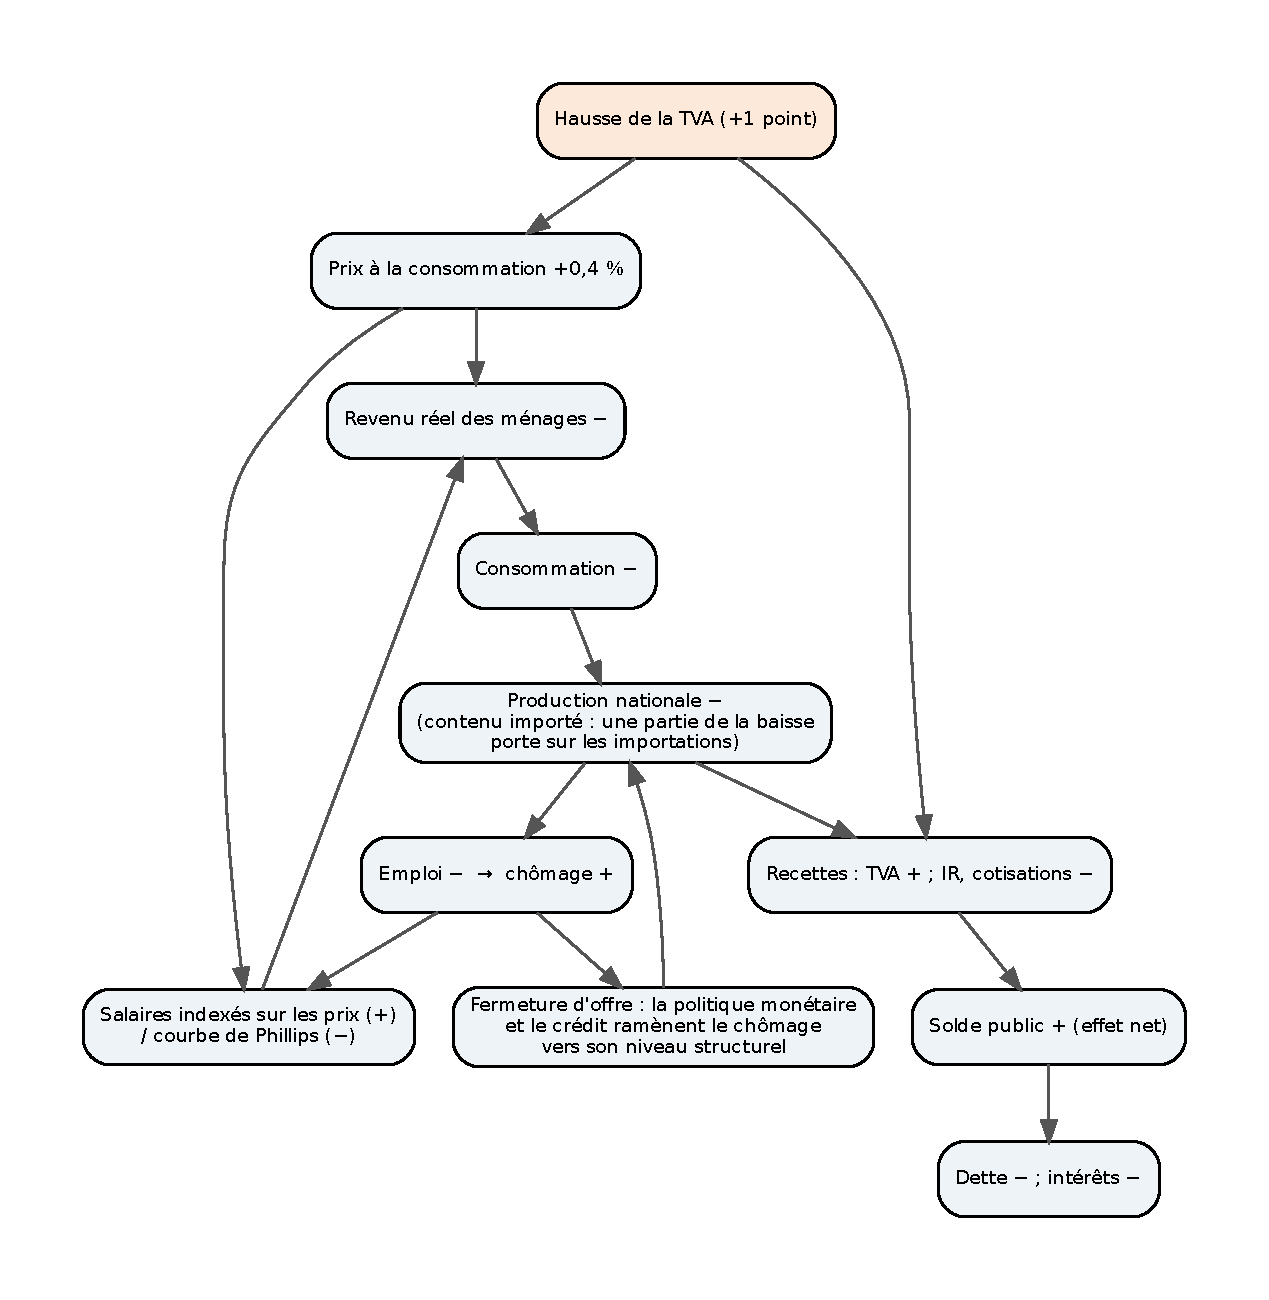
\includegraphics[width=0.78\linewidth]{chaine_causale.pdf}
\caption{Exemple de propagation : hausse d'un point du taux normal de TVA. Chaque case correspond à une ou plusieurs
équations du modèle ; les ordres de grandeur sont ceux de la simulation du chapitre~\ref{ch:experiences}.}
\label{fig:chaine}
\end{figure}

\begin{exemple}[Exemple : la propagation d'une hausse de TVA (simulation « TVA +1 point »)]
Un point de TVA rapporte statiquement environ 8,2\md{} (80~\% de la recette nette au taux normal, rapportée au taux).
Le modèle suppose qu'il est répercuté à 80~\% sur les prix : les prix à la consommation sont plus élevés de 0,42~\% en
2030. Le pouvoir d'achat des ménages baisse de 0,29~\% ; la consommation de 0,28~\%. Une partie de cette consommation
perdue portait sur des produits importés (27~\% en moyenne du contenu de la consommation) : la production nationale ne
baisse que de 0,09~\% en 2029. L'emploi recule de 23\,000 postes, le chômage monte de 0,08 point. Les
salaires, indexés en partie sur les prix, augmentent de 0,09~\%, ce qui amortit la perte de pouvoir d'achat mais
renchérit le coût du travail. Côté finances publiques, la recette nouvelle (+0,34 point de PIB de recettes) est
partiellement compensée par les moindres recettes d'impôt sur le revenu et de cotisations liées à l'activité : le
solde public s'améliore de 0,21 point de PIB en 2029, 0,24 en 2032. La dette est plus basse de 2,2 points de PIB en
2037, grâce aussi à l'effet du niveau des prix sur le PIB nominal. À long terme, la fermeture d'offre ramène l'activité
vers son niveau de référence (PIB $-$0,02~\% en 2037).
\end{exemple}

\section{Niveaux de preuve}
\label{sec:niveaux}

Chaque paramètre et chaque résultat de ce rapport est qualifié par un niveau de preuve, repris du registre des
paramètres du projet (annexe~\ref{ann:registre}) :

\begin{center}\small
\begin{tabularx}{0.95\linewidth}{@{}lL@{}}
\toprule
Code & Signification \\
\midrule
\preuve{R} & Relation comptable : vraie par définition. \\
\preuve{A} & Donnée observée (comptes nationaux, législation, statistiques publiques). \\
\preuve{E} & Coefficient estimé économétriquement sur des données françaises (avec son écart-type). \\
\preuve{C} & Calibré sur une source empirique française ou une méta-analyse. \\
\preuve{L} & Transposé de la littérature (souvent étrangère). \\
\preuve{H} & Hypothèse de modélisation, sans mesure empirique directe. \\
\bottomrule
\end{tabularx}
\end{center}

Pour les résultats, on utilise une échelle de robustesse : \fiab{robuste} (signe et ordre de grandeur stables dans
tous les tests de sensibilité), \fiab{plutôt robuste} (signe stable, ampleur variable), \fiab{fragile} (signe
dépendant d'hypothèses), \fiab{non établi} (le modèle ne permet pas de conclure).

\chapter{Documentation des sous-modèles}
\label{ch:sousmodeles}

Ce chapitre documente chaque mécanisme du modèle selon une structure fixe : \textbf{A} ce que le sous-modèle
représente ; \textbf{B} les variables ; \textbf{C} les hypothèses ; \textbf{D} les équations, telles qu'elles sont
codées ; \textbf{E} la calibration ; \textbf{F} les limites. Les équations reprennent les notations du code
(fichiers \code{src/m7\_equations.py} et \code{src/m8\_modele.py}). Les coefficients sont ceux de la version 0.6 ;
les écarts-types figurent entre parenthèses. Conventions : $\ln$ est le logarithme népérien ; $\Delta \ln X_t =
\ln X_t - \ln X_{t-1}$ est, à peu de chose près, le taux de croissance de $X$ ; l'indice $b$ désigne une branche,
$t$ une année, $B = 2022$ l'année de base.

\begin{encadre}{Encadré 2.1 — Lire une équation « à correction d'erreur »}
La plupart des équations de comportement ont la même forme :
\[
\Delta \ln Y_t = \underbrace{a\,\Delta \ln X_t}_{\text{réaction immédiate}}
\;+\; \underbrace{\lambda\,\bigl(\ln Y_{t-1} - \ln Y^{*}_{t-1}\bigr)}_{\text{rappel vers l'équilibre}} \;+\; c ,
\qquad \lambda < 0 .
\]
Le premier terme dit comment $Y$ réagit \emph{la première année} à une variation de $X$ ; le second ramène
progressivement $Y$ vers sa valeur d'équilibre $Y^{*}$ (par exemple, la consommation vers une part stable du revenu).
Si $\lambda = -0{,}22$, l'écart à l'équilibre se réduit de 22~\% chaque année : il en reste la moitié au bout de
trois ans environ ($0{,}78^3 \approx 0{,}47$). Ce type d'équation, dit « à correction d'erreur » (MCE), est la forme
standard des modèles macro-économétriques depuis les travaux d'Engle et Granger (1987).
\end{encadre}

\section{Démographie et population active (M1, M9)}
\label{sec:m1}

\paragraph{A. Objet.} La démographie fixe deux grandeurs décisives pour l'économie : le nombre de personnes en âge
de travailler (et donc l'offre de travail) et le nombre de retraités (et donc la masse des pensions). Le rapport entre
les deux conditionne la soutenabilité du système social.

\paragraph{B. Variables.} $P_{s,a,t}$ : population au 1\textsuperscript{er} janvier par sexe $s$ et âge révolu
$a$ (0 à 120 ans) ; $q_{s,a,t}$ : quotients de mortalité ; $f_{a,t}$ : taux de fécondité ; $SM_{s,a,t}$ : solde
migratoire ; $\tau_{s,a}$ : taux d'activité ; $AOD_g$ : âge d'ouverture des droits à la retraite de la génération $g$.
Source : Insee, projections de population 2026 \src{Insee, projections 2026} ; Eurostat \code{lfsa\_argan} (taux d'activité).

\paragraph{C. Hypothèses.} Le module applique les hypothèses centrales de l'Insee : fécondité de 1,45 enfant par
femme à partir de 2028, solde migratoire de +150\,000 personnes par an, gains d'espérance de vie au rythme 2005-2025
(89,5 ans pour les femmes et 86,7 ans pour les hommes en 2070). Les taux d'activité par sexe et âge avant 55 ans
restent à leur niveau de 2024 ; ceux de 55 à 74 ans dépendent de l'âge légal (M9).

\paragraph{D. Équations.} Méthode des composantes (diagramme de Lexis) :
\begin{align}
P_{s,A,t+1} &= P_{s,A-1,t}\,(1-q_{s,A,t}) + SM_{s,A,t}\,\bigl(1-\tfrac{q_{s,A,t}}{2}\bigr) + AJ_{s,A,t} \\
N_t &= \sum_{A=15}^{50} f_{A,t}\,\frac{P^F_{A-1,t}+P^F_{A,t+1}}{2},\qquad P_{s,0,t+1} = N_t\,\pi_s\,(1-q_{s,0,t})+\dots \\
\text{Actifs}_t &= \sum_{s}\sum_{a} P_{s,a,t}\,\tau_{s,a}
\end{align}
avec $\pi_F = 100/205$ la part des filles à la naissance et $AJ$ l'ajustement statistique de l'Insee (nul après 2028).
L'identité $P_{t+1}-P_t = N_t - D_t + SM_t + AJ_t$ est contrôlée à chaque pas (tolérance 0,001 personne).

Pour les seniors (M9), le taux d'activité de 55 à 74 ans est exprimé relativement à celui des 50-54 ans et dépend de
l'écart entre l'âge et l'$AOD$ de la génération. Avant l'$AOD$ : sorties précoces en rampe sur 5 ans (carrières
longues, invalidité, chômage) ; après l'$AOD$ : une part reste active puis décroît exponentiellement. Un paramètre
$\beta$ mesure la part du profil qui se décale avec l'âge légal (la part $1-\beta$ reste attachée à 62 ans).

\begin{exemple}
Relever l'âge légal d'un an décale environ les trois quarts ($\beta \approx 0{,}75$) des départs d'un an. Sur une
génération de 800\,000 personnes dont 60~\% sont encore actives à 62 ans, cela maintient environ
$0{,}75 \times 0{,}6 \times 800\,000 \approx 360\,000$ personnes-années d'activité supplémentaires par génération concernée.
Avec $\beta = 1$ (décalage complet), l'effet serait d'un tiers plus fort ; avec $\beta = 0{,}5$, d'un tiers plus faible.
\end{exemple}

\paragraph{E. Calibration.} Démographie : aucun paramètre calé, les hypothèses publiées sont appliquées ; le module
reproduit les 29 scénarios de l'Insee à moins de $3{,}4\cdot10^{-5}$ près sur la population totale 2024-2070
\preuve{A}. Activité des seniors : estimation par moindres carrés non linéaires sur l'enquête Emploi 2003-2019 ;
$\beta = 0{,}78$ (femmes) et $0{,}75$ (hommes), erreur quadratique moyenne 1,0 à 1,1 point \preuve{E}. Hors
échantillon (2020-2025, relèvement de l'AOD de 62 ans à 62 ans et 9 mois), l'écart est de 0 à 3 points pour les
60-64 ans. Sur 2010-2019, neuf seniors maintenus actifs sur dix étaient en emploi (rapport $\Delta$ taux
d'emploi / $\Delta$ taux d'activité = 0,89).

\paragraph{F. Limites.} Pas de durée d'assurance, de décote ni de surcote ; taux d'activité avant 55 ans figés ; la
fécondité et les migrations ne réagissent pas à l'économie ; l'enquête Emploi a connu une rupture de série en 2021.

\section{Production, branches et échanges entre produits (M5)}
\label{sec:m5}

\paragraph{A. Objet.} Produire une voiture demande de l'acier, de l'électricité, du transport, des services : chaque
branche achète aux autres. Le tableau entrées-sorties décrit ces échanges et permet de calculer combien de production,
d'importations et d'emplois sont mobilisés, directement et indirectement, par un euro de demande finale.

\paragraph{B. Variables.} $x$ : production par produit (64 produits, nomenclature A64) ; $f^d$ : demande finale
adressée à la production intérieure ; $A^d$, $A^m$ : coefficients techniques des consommations intermédiaires
intérieures et importées ; $a^v$ : valeur ajoutée par unité produite ; $p$ : prix de production ; $p^m$ : prix
d'importation ; $\varphi$ : facteur commun d'ajustement des parts importées. Source : Eurostat
\code{naio\_10\_cp1700} (tableau symétrique, 2010-2022), \code{naio\_10\_cp15} (prix d'importation).

\paragraph{C. Hypothèses.} Coefficients techniques fixes à l'année de base 2022 : pas de substitution entre
intrants ni entre produit français et importé, sauf par le facteur commun $\varphi$ qui ajuste toutes les parts
importées (sauf l'énergie, non concurrente) pour respecter l'équation agrégée d'importations (section~\ref{sec:commerce}).

\paragraph{D. Équations.}
\begin{align}
x &= \bigl(I - A^d(\varphi)\bigr)^{-1} f^d(\varphi), \qquad m = A^m(\varphi)\,x + f^m(\varphi) \\
p &= \bigl(p^m A^m + p^v a^v\bigr)\bigl(I - A^d\bigr)^{-1}
\end{align}
où $p^v$ est le prix de la valeur ajoutée unitaire de la branche productrice (salaires, marges, impôts sur la
production). La valeur ajoutée de la branche $b$ en volume est $Q_b = \sum_{p\in b} a^v_p x_p$.

\begin{exemple}
Le contenu en importations de la demande finale intérieure est de 0,18~€ par euro en 2021 ; il atteint 0,73 pour les
produits raffinés, 0,52 pour l'aéronautique et les autres matériels de transport, 0,50 pour la métallurgie et 0,48 pour
l'automobile \src{validation M5}. Une hausse de 50~\% des prix de l'énergie importée, à marges fixes, élève les prix de
production de 1,3~\% et les prix à la consommation de 1,7~\%.
\end{exemple}

\paragraph{E. Calibration.} Observé \preuve{A/R} : identités vérifiées à 2\,M€ près pour 2010-2022. Test des prix
2012-2019 avec les prix de valeur ajoutée observés : erreur de 0,3 à 0,8 point par produit, corrélation de 0,89 à 0,98.

\paragraph{F. Limites.} En 2022, le modèle de prix à coefficients fixes surestime fortement la hausse de certains
prix (raffinage +74~\% prévu contre +43~\% observé), faute de substitutions et de variations de marges ; le tableau
2022 est le dernier publié (2023-2024 vides chez Eurostat).

\section{Emploi et chômage}
\label{sec:emploi}

\paragraph{A. Objet.} Les entreprises ajustent leurs effectifs à leur production, avec retard, et selon le coût réel
du travail. Le chômage est la part de la population active sans emploi.

\paragraph{B. Variables.} $N_{b,t}$ : emploi de la branche (personnes, milliers) ; $Q_{b,t}$ : valeur ajoutée en
volume ; $CN_{b,t}$ : coût salarial par tête ; $PVA_{b,t}$ : prix de la valeur ajoutée ; $g_b$ : tendance de
productivité de la branche ; $u_t$ : taux de chômage (France métropolitaine, BIT) ; $PA_t$ : population active.
Sources : Eurostat \code{nama\_10\_a64}, \code{nama\_10\_a64\_e} ; Insee, série 001688526.

\paragraph{C. Hypothèses.} Rendements d'échelle constants à long terme (l'emploi est proportionnel à la production,
corrigé de la productivité) ; élasticité de substitution entre capital et travail $\sigma = 0{,}4$ ; les emplois non
marchands sont proportionnels au volume de la production non marchande ; la productivité tendancielle par branche est
celle des huit dernières années observées.

\paragraph{D. Équations.} Pour chaque branche marchande :
\begin{multline}
\Delta\ln N_{b,t} = c_b + \underset{(0{,}043)}{0{,}259}\,\Delta\ln Q_{b,t} + \underset{(0{,}018)}{0{,}012}\,\Delta\ln Q_{b,t-1}
+ \underset{(0{,}057)}{0{,}317}\,\Delta\ln N_{b,t-1} \\
\underset{(0{,}031)}{-\,0{,}206}\Bigl[\ln N_{b,t-1} - \ln Q_{b,t-1} + \sigma\,\ln\frac{CN_{b,t-1}}{PVA_{b,t-1}} + g_b\,(t-1-B)\Bigr]
\end{multline}
\begin{equation}
u_t = 100\left(1 - \frac{\sum_b N_{b,t} + N^{nm}_t}{PA_t}\right)
\end{equation}
Le crochet est l'écart entre l'emploi et son niveau d'équilibre $\ln N^* = \ln Q - \sigma \ln(CN/PVA) - g_b\,t$.

\begin{exemple}
Si la production d'une branche augmente durablement de 1~\%, l'emploi augmente de 0,26~\% la première année, puis de
0,26~\% $\times$ 0,317 par inertie et de 21~\% de l'écart restant par le rappel : environ +0,5~\% au bout de deux ans,
+0,9~\% au bout de six. Si le coût réel du travail augmente de 1~\%, l'emploi d'équilibre baisse de $\sigma = 0{,}4$~\%.
Avec $\sigma = 0{,}2$ (bas de la littérature), une hausse des salaires détruit deux fois moins d'emplois ; avec
$\sigma = 0{,}7$, presque deux fois plus.
\end{exemple}

\paragraph{E. Calibration.} Estimé sur 25 branches, 1997-2019, effets fixes et tendances de branche \preuve{E}.
L'élasticité de long terme à la production est imposée à 1 (la version libre donne 0,44, biaisée par la colinéarité
avec les tendances). $\sigma = 0{,}4$ est \preuve{C} : non identifié sur les données (estimation libre $-$0,21, non
robuste), fixé au milieu des estimations françaises (0,2 à 0,7).

\paragraph{F. Limites.} Une seule élasticité pour tous les niveaux de qualification : le modèle ne représente pas la
sensibilité plus forte de l'emploi peu qualifié au coût du travail, documentée par les évaluations des allègements de
cotisations (Kramarz et Philippon, 2001). Il sous-estime donc probablement l'effet des allègements ciblés et l'effet
d'une hausse du SMIC sur l'emploi peu qualifié. Pas de flux d'embauches et de licenciements, pas d'appariement, pas
d'automatisation au-delà de la substitution capital-travail ($\sigma$).

\section{Formation des salaires}
\label{sec:salaires}

\paragraph{A. Objet.} Le salaire moyen s'ajuste aux prix (indexation, négociations), à la productivité, et à l'état du
marché du travail (un chômage élevé modère les salaires : courbe de Phillips).

\paragraph{B. Variables.} $W_t$ : salaire moyen par tête du secteur marchand ; $PC_t$ : prix de la consommation ;
$PROD_t$ : productivité par tête ; $PVA^m_t$ : prix de la valeur ajoutée marchande ; $u^*_t$ : chômage structurel
(7,5~\% en projection).

\paragraph{D. Équation.}
\begin{multline}
\Delta\ln W_t = c + \underset{(0{,}222)}{0{,}394}\,\Delta\ln PC_t + \underset{(0{,}120)}{0{,}032}\,\Delta\ln PROD_t \\
\underset{(0{,}057)}{-\,0{,}093}\bigl[\ln W_{t-1} - \ln PVA^m_{t-1} - \ln PROD_{t-1}\bigr] \;-\; 0{,}004\,(u_{t-1}-u^*_t)
\end{multline}
Le crochet est (le logarithme de) la part des salaires dans la valeur ajoutée : si elle est au-dessus de sa norme, les
salaires ralentissent.

\begin{exemple}
Une inflation de 2~\% augmente les salaires de 0,8~\% la même année ; le reste est rattrapé à raison de 9~\% de l'écart
par an, si bien que la part des salaires revient à sa norme en une dizaine d'années. Un point de chômage au-dessus du
niveau structurel freine la croissance des salaires de 0,4 point par an.
\end{exemple}

\paragraph{E. Calibration.} Indexation et rappel estimés \preuve{E} (l'indexation a un $t$ de 1,8 seulement).
Effet du chômage \preuve{C} : l'estimation libre donne un effet positif (+0,0066), biaisé par la composition de
l'emploi (les emplois à bas salaire disparaissent d'abord en récession, ce qui augmente mécaniquement le salaire
moyen) ; la valeur retenue ($-$0,4~\% par point) est dans la fourchette des estimations françaises.

\paragraph{F. Limites.} Un seul salaire moyen : pas de distinction entre SMIC et autres salaires, ni entre secteurs
exposés et abrités. Une hausse du SMIC est représentée par sa diffusion supposée à la masse salariale (0,11 pour 1,
hypothèse \preuve{H}) et par son coût public direct (allègements indexés sur le SMIC : 0,66\md{} par point).

\section{Prix et inflation}
\label{sec:prix}

\paragraph{A. Objet.} Les entreprises fixent leurs prix en appliquant une marge à leurs coûts ; les hausses de prix
importés (énergie notamment) se transmettent avec retard.

\paragraph{D. Équations.} Prix de la valeur ajoutée de chaque branche, en fonction du coût salarial unitaire
$CSU_b = CN_b N_b / Q_b$ :
\begin{multline}
\Delta\ln PVA_{b,t} = c_b + \underset{(0{,}113)}{0{,}670}\,\Delta\ln CSU_{b,t} + \underset{(0{,}072)}{0{,}109}\,\Delta\ln Q_{b,t}
+ \underset{(0{,}001)}{0{,}0015}\,TUCD_{b,t} \\ \underset{(0{,}057)}{-\,0{,}117}\bigl[\ln PVA_{b,t-1} - \ln CSU_{b,t-1} - mk_{b,t-1}\bigr] + \Delta mk_{b,t}
\end{multline}
où $TUCD$ est l'écart du taux d'utilisation des capacités à sa moyenne (branches industrielles) et $mk$ un choc de
marge éventuel (impôts de production, droits de douane). Transmission des prix d'importation, par produit :
\begin{equation}
\ln p^{m,\text{eff}}_t = \ln p^{m,\text{eff}}_{t-1} + \theta\,\bigl(\ln p^m_t - \ln p^{m,\text{eff}}_{t-1}\bigr),\qquad \theta = \underset{(\text{estimé})}{0{,}495}.
\end{equation}
Les prix de la consommation, de l'investissement et des exportations sont ensuite les moyennes, pondérées par les
structures du tableau entrées-sorties, des prix de production $p$ (section~\ref{sec:m5}) et des prix importés
répercutés.

\begin{exemple}
Une hausse de 10~\% des prix de l'énergie importée n'est répercutée qu'à moitié la première année ($\theta \approx 0{,}5$),
aux trois quarts la deuxième. Une hausse de 1~\% du coût salarial unitaire relève le prix de la valeur ajoutée de
0,67~\% la première année, puis entièrement à long terme (homogénéité imposée).
\end{exemple}

\paragraph{E. Calibration.} \preuve{E} sur 1997-2019 pour les prix de valeur ajoutée (la version libre donne une
transmission de long terme de 0,74 au lieu de 1 imposé) ; $\theta$ estimé sur 1998-2024 : sur 1998-2019, la
transmission était immédiate ; le délai n'apparaît qu'avec l'épisode énergétique de 2021-2024 (tarifs réglementés,
bouclier tarifaire, contrats).

\paragraph{F. Limites.} Pas de prix de marché de l'électricité ni de mécanisme de reconstitution de marges ; le
modèle a sous-estimé les prix de 2,8~\% sur 2023-2024 (validation M8).

\section{Consommation et épargne des ménages (M7, M14)}
\label{sec:conso}

\paragraph{A. Objet.} La consommation des ménages (la moitié du PIB) dépend avant tout de leur revenu réel. Les
ménages modestes dépensent une part plus grande d'un euro supplémentaire que les ménages aisés.

\paragraph{B. Variables.} $C_t$ : consommation en volume ; $RDB_t$ : revenu disponible brut (M€ courants) ;
$RDB^{\text{eff}}_t$ : revenu « effectif » corrigé de l'hétérogénéité ; $PC_t$ : prix de la consommation ; taux
d'épargne $s_t = (RDB_t - PC_t C_t)/RDB_t$.

\paragraph{D. Équations.}
\begin{equation}
\Delta\ln C_t = c + \underset{(0{,}205)}{0{,}853}\,\Delta\ln\frac{RDB^{\text{eff}}_t}{PC_t} \;\underset{(0{,}211)}{-\,0{,}218}\Bigl[\ln C_{t-1} - \ln\frac{RDB^{\text{eff}}_{t-1}}{PC_{t-1}}\Bigr]
\end{equation}
\begin{equation}
RDB^{\text{eff}}_t = RDB_t + \sum_{d=1}^{10} \Delta R_{d,t}\Bigl(\frac{\pi_d}{\bar\pi}-1\Bigr) + \Delta Div^{\text{mén}}_t\Bigl(\frac{\pi_{\text{top 1}}}{\bar\pi}-1\Bigr)
\end{equation}
où $\Delta R_d$ est la variation du revenu du décile $d$ due à la mesure (microsimulation), $\pi_d$ la propension
marginale à consommer du décile (0,90 ; 0,85 ; 0,80 ; 0,75 ; 0,72 ; 0,68 ; 0,64 ; 0,60 ; 0,53 ; 0,40), $\bar\pi$ sa moyenne
pondérée par le revenu, et $\pi_{\text{top 1}} = 0{,}25$ la propension du dernier centile, appliquée aux dividendes.

\begin{exemple}
Un transfert de 1\md{} aux ménages du premier décile compte pour $1 \times 0{,}90/\bar\pi \approx 1{,}38$\md{} dans
l'équation de consommation ($\bar\pi \approx 0{,}65$) ; une baisse d'impôt de 1\md{} pour le dixième décile ne compte
que pour $0{,}40/0{,}65 \approx 0{,}62$\md. À montant égal, la première mesure soutient donc environ deux fois plus la
consommation la première année. Seul le \emph{profil relatif} des propensions intervient : la propension moyenne reste
celle de l'équation estimée.
\end{exemple}

\paragraph{E. Calibration.} Équation agrégée \preuve{E} (1997-2019) ; l'élasticité de court terme varie de 0,54 à 1,15
selon la période d'estimation et la force de rappel n'est pas significative ($t = -1{,}0$). Profil des propensions
\preuve{C} : cohérent avec les taux d'épargne par quintile de l'Insee (de $-$29~\% pour le premier quintile à 27~\% pour le
cinquième en 2022) \src{Insee Focus n\textsuperscript{o} 338, 2024} et avec Garbinti et Lamarche (2014) ; variantes
« plat » et « accentué » en sensibilité.

\paragraph{F. Limites.} Pas d'effet de richesse, de taux d'intérêt, d'épargne de précaution ni d'anticipation
(pas d'« équivalence ricardienne ») ; pas de distinction entre revenu permanent et temporaire (une prime ponctuelle a
probablement un effet d'un tiers plus faible la première année que celui simulé) ; le taux d'épargne de référence
(17,9~\% en 2025, ramené à 15,5~\% à long terme) est une hypothèse de projection.

\section{Investissement et accumulation du capital}
\label{sec:invest}

\paragraph{A. Objet.} Les entreprises investissent pour répondre à la demande (effet d'accélérateur) et d'autant plus que
le coût du capital (taux d'intérêt, impôt sur les sociétés) est bas. Les ménages investissent dans le logement selon
leur revenu. Le capital installé détermine les capacités de production.

\paragraph{D. Équations.} Investissement de la branche $b$ (hors effet du coût du capital), puis effet du coût d'usage
$CU$ appliqué en niveau :
\begin{multline}
\Delta\ln \tilde I_{b,t} = c_b + \underset{(0{,}204)}{0{,}670}\,\Delta\ln Q_{b,t} + \underset{(0{,}097)}{0{,}256}\,\Delta\ln Q_{b,t-1}
\underset{(0{,}109)}{-\,0{,}285}\ln \tilde I_{b,t-1} + \underset{(0{,}096)}{0{,}192}\ln K_{b,t-1} + \underset{(0{,}048)}{0{,}113}\ln Q_{b,t-1}
\end{multline}
\begin{equation}
CU_t = \frac{r_t + \delta}{1-\tau^{IS}_t},\qquad \ln m_t = \ln m_{t-1} + 0{,}285\,\bigl(\varepsilon\,[\ln CU_t - \ln CU_B] - \ln m_{t-1}\bigr),\qquad I_{b,t} = \tilde I_{b,t}\, m_t
\end{equation}
avec $\delta = 0{,}07$, $\varepsilon = -0{,}184$ (élasticité de long terme estimée sur l'investissement des sociétés
non financières, écart-type de $\lambda$ 0,14). Capital : $K_{b,t} = (1-\delta_b)K_{b,t-1} + I_{b,t} + I^{\text{cap}}_{b,t}$.
Logement des ménages :
\begin{equation}
\Delta\ln I^{\text{mén}}_t = c + \underset{(0{,}35)}{1{,}48}\,\Delta\ln\frac{RDB_t}{PC_t} \underset{(0{,}20)}{-\,0{,}282}\Bigl[\ln I^{\text{mén}}_{t-1}-\ln\frac{RDB_{t-1}}{PC_{t-1}}\Bigr]
\end{equation}
L'investissement public est exogène : chaque milliard supplémentaire s'ajoute à la demande et, par une élasticité de
la production au capital public de 0,08 (capital public net égal à 55~\% du PIB, dépréciation de 4~\% par an,
productif l'année suivant la dépense), à la productivité.

\begin{exemple}[Exemple : baisse de l'impôt sur les sociétés de 25 \% à 20 \%]
$1-\tau$ passe de 0,75 à 0,80 : le coût d'usage baisse de $\ln(0{,}80/0{,}75) = 6{,}5~\%$. L'investissement de long
terme augmente de $0{,}184 \times 6{,}5 \approx 1{,}2~\%$, dont 28~\% la première année (0,34~\%). Avec
$\varepsilon = -0{,}4$ (haut de la littérature internationale), l'effet doublerait ; avec $\varepsilon = -0{,}1$, il
serait presque divisé par deux. La recette d'IS perdue (environ 12\md{} de gain statique pour les entreprises) n'est
pas récupérée par l'activité supplémentaire (chapitre~\ref{ch:experiences}).
\end{exemple}

\paragraph{E. Calibration.} Accélérateur \preuve{E} ; élasticité au coût d'usage \preuve{E, fragile} (23 observations,
prévision hors échantillon médiocre) ; élasticité au capital public \preuve{L} (méta-analyse de Bom et Ligthart, 2014 ;
plage 0,04-0,12).

\paragraph{F. Limites.} L'effet du taux de marge sur l'investissement, estimé positif mais non significatif ($t=1{,}4$),
n'est pas utilisé ; pas de contrainte de financement ni d'effet de trésorerie ; aucune dépense publique autre que
l'investissement (éducation, recherche, santé) n'a d'effet sur la productivité ; l'investissement de capacité de la
réindustrialisation est décidé de façon exogène.

\section{Productivité, capacités et croissance potentielle}
\label{sec:fermeture}

\paragraph{A. Objet.} À long terme, la production est limitée par la quantité de travail et de capital disponibles et par
leur efficacité. Un modèle tiré par la demande doit donc être « fermé » par un mécanisme qui ramène l'économie vers son
potentiel : politique monétaire, crédit, compétitivité.

\paragraph{C. Hypothèses.} (1) La productivité tendancielle de chaque branche est un paramètre de scénario (moyenne
des 8 dernières années observées ; 0,7~\% par tête pour l'ensemble de l'économie après 2031, hypothèse centrale du COR).
(2) Le taux d'utilisation des capacités de l'industrie influence (faiblement) les prix. (3) \textbf{Fermeture d'offre}
\preuve{H} : un supplément de demande intérieure $Z$ (60~\% consommation, 40~\% investissement) ramène progressivement
le chômage vers son niveau structurel $u^*$.

\paragraph{D. Équations.}
\begin{equation}
Z_t = Z_{t-1} + \Bigl[\rho\,(u_{t-1}-u^*) + 0{,}3\,\bigl((u_{t-1}-u^*)-(u_{t-2}-u^*)\bigr)\Bigr]\times\frac{1{,}5}{100},\qquad \rho = 0{,}15
\end{equation}
$Z$ est exprimé en part de la production totale ; 1,5 est le coefficient d'Okun (points de PIB par point de chômage).
C'est un correcteur « proportionnel-intégral » : tant que le chômage est au-dessus de $u^*$, la demande supplémentaire
s'accumule. Taux d'utilisation des capacités : $TUC_{b,t} = TUC_{b,B}\,(Q_{b,t}/Q_{b,B})/(K_{b,t-1}e^{g^k_b(t-B)}/K_{b,B-1})$.

\begin{exemple}
Une mesure qui augmente le chômage de 0,3 point déclenche chaque année un supplément de demande de
$0{,}15\times0{,}3\times1{,}5 = 0{,}07$ point de PIB, qui s'accumule : au bout de cinq ans, environ 0,25 point de PIB, ce
qui ramène le chômage vers sa valeur de départ. Avec $\rho = 0$ (vision « keynésienne » : rien ne ramène l'économie
au plein emploi), les effets de demande sont permanents ; avec $\rho = 0{,}4$, ils disparaissent en trois à quatre ans.
\end{exemple}

\paragraph{E. Calibration.} $\rho$ n'est pas estimé : il est choisi pour que les multiplicateurs de dépense publique
décroissent comme dans Mésange et FR-BDF (1,2 la première année, 0,85 la deuxième, 0,6 à cinq ans). \textbf{C'est le
premier facteur d'incertitude du modèle} sur le PIB et l'emploi à moyen terme (criblage de Morris, contre-expertise
v0.6).

\paragraph{F. Limites.} Mécanisme réduit et symétrique ; pas de politique monétaire nationale (zone euro) autre que
celle du module M11 ; pas d'hystérèse (un chômage durablement élevé ne dégrade pas le potentiel) ; la productivité ne
dépend ni de l'éducation, ni de la recherche, ni de l'automatisation, ni du temps de travail au-delà d'une hypothèse de
compensation (section~\ref{sec:catalogue}).

\section{Commerce extérieur, énergie et dépendances}
\label{sec:commerce}

\paragraph{A. Objet.} Les importations augmentent avec la demande (surtout l'investissement et les exportations, riches
en contenu importé) ; les exportations dépendent de la demande mondiale et de la compétitivité-prix.

\paragraph{D. Équations.} Importations totales en volume :
\begin{multline}
\Delta\ln M_t = c + \underset{(0{,}092)}{1{,}465}\,\Delta\ln D_t \underset{(0{,}101)}{-\,0{,}114}\,\Delta\ln\frac{PM^{nc}_t}{PPIB_t} \\
\underset{(0{,}149)}{-\,0{,}661}\Bigl[\ln M_{t-1} - 1{,}370\ln D_{t-1} + 0{,}163\ln\frac{PM^{nc}_{t-1}}{PPIB_{t-1}}\Bigr] + 0{,}0039\,t
\end{multline}
avec $D_t = 0{,}13\,C_t + 0{,}06\,G_t + 0{,}23\,(I_t+S_t) + 0{,}33\,X_t$ (demande pondérée par le contenu en importations,
en indices) et $PM^{nc}$ le prix des importations hors énergie (non concurrente). Exportations :
\begin{equation}
\Delta\ln X_t = c + \underset{(0{,}094)}{0{,}711}\,\Delta\ln DM_t \underset{(0{,}171)}{-\,0{,}595}\,\Bigl(\Delta\ln PX_t - \Delta\ln PW_t\Bigr)
\end{equation}
où $DM$ est la demande mondiale adressée (importations de l'Union européenne) et $PW$ le prix des concurrents. Le total
importé est réparti entre produits par le facteur $\varphi$ (section~\ref{sec:m5}) ; l'énergie (produits B, C19, D)
est non concurrente : sa part importée ne varie pas.

\begin{exemple}
Une hausse de 1~\% de la demande pondérée augmente les importations de 1,47~\% la première année. Une perte de
compétitivité-prix de 1~\% réduit les exportations de 0,6~\%, mais les importations de seulement 0,11~\% : le modèle
représente mieux la perte de marchés à l'exportation que la conquête du marché intérieur par les importations.
\end{exemple}

\paragraph{E. Calibration.} \preuve{E}, 1997-2019. L'élasticité-prix des importations ($-$0,11 à court terme, $-$0,16 à
long terme) est non significative et plus faible que la littérature ($-$0,3 à $-$0,6). Celle des exportations est
conforme aux estimations françaises ($-$0,4 à $-$0,8).

\paragraph{F. Limites.} Pas de taux de change hors zone euro ; pas de traitement spécifique des grands contrats
(aéronautique), ce qui explique l'erreur de 2023 ; dépendances matérielles représentées seulement en valeur (pas de
métaux critiques, pas de goulets physiques) ; pas de substitution entre énergies ni d'effet de la taxe carbone sur les
émissions.

\section{Revenus des ménages, profits et revenus versés au reste du monde}
\label{sec:revenus}

\paragraph{D. Équations.} Le revenu disponible brut est la somme de composantes indexées :
\begin{equation}
RDB_t = \underbrace{D1_B\,\frac{W_t}{W_B}\frac{N_t}{N_B}}_{\text{salaires}} + \underbrace{EBE^{mén}_t + D4_t}_{\text{patrimoine, indépendants}}
+ \underbrace{D62_t}_{\text{prestations}} + \text{autres}_t - \underbrace{D61_t}_{\text{cotisations}} - \underbrace{D5_t}_{\text{impôts}}
\end{equation}
Les prestations sont indexées sur les prix de l'année précédente et sur un volume exogène (pensions par M9 ; autres
prestations +1,4~\% par an, rythme 2011-2019). Les cotisations sont proportionnelles aux salaires, les impôts à la base
imposable (salaires, patrimoine, prestations). Les revenus du patrimoine et l'excédent des ménages suivent des équations
estimées sur le PIB nominal, les prix et le taux long :
\begin{equation}
\Delta\ln D4_t = c + 0{,}874\,\Delta\ln PIBN_t + 3{,}05\,\Delta\ln PC_t - 0{,}366\,[\ln D4_{t-1}-\ln PIBN_{t-1}] + 0{,}021\,r_{t-1}
\end{equation}
Profits (M14) : un supplément de profit après impôt $\Pi$ (baisse d'IS ou d'impôts de production) est distribué à
50~\% (plage 30-70~\%) ; 30~\% des dividendes vont aux non-résidents (plage 20-50~\%), 35~\% du reste directement aux
ménages résidents ; le solde est conservé par les entreprises. Le revenu national brut est $RNB = PIBN + R^{prim}$,
où $R^{prim}$ (revenus primaires nets reçus du reste du monde) vaut 3,1~\% du PIB à l'année de base, diminué des
dividendes supplémentaires versés à l'étranger.

\paragraph{F. Limites.} En 2023-2024, le RDB est sous-estimé de 7,9~\% en rétrosimulation : les revenus de la propriété
(+15~\% par an avec la hausse des taux) ne suivent pas le PIB nominal ; le niveau de solde extérieur du modèle
n'est pas fiable (chapitre~\ref{ch:reference}).

\section{Fiscalité des ménages (M4, M10, M13)}
\label{sec:fiscmen}

\paragraph{A. Objet.} Calculer, ménage par ménage, l'impôt sur le revenu, la CSG et les prestations, puis en déduire
la recette publique, la variation de revenu par décile et l'effet sur la pauvreté.

\paragraph{B. Données.} Échantillon de 2~\% des ménages ordinaires du fichier détail du recensement 2022 (163\,826
ménages, 344\,527 personnes, 201\,821 foyers fiscaux) ; revenus attribués par rang à partir de la distribution du revenu
fiscal de référence publiée par la DGFiP (IRCOM 2025, revenus 2024, 25 tranches) ; statistiques nationales par case de
déclaration (heures supplémentaires, revenus de l'étranger, épargne retraite) ; législation par OpenFisca-France.

\paragraph{C. Hypothèses.} Rang de revenu tiré de grilles publiées (salaires par catégorie socioprofessionnelle et sexe,
pensions) ; revenus du capital concentrés vers le haut ; non-recours aux prestations constant (taux apparents mesurés :
RSA 0,68 ; prime d'activité 0,66).

\paragraph{D. Calcul.} Pour une réforme $R$ : $\Delta T = \sum_h w_h\,[T_h(R) - T_h(\text{actuel})]$, ramené aux 41,6
millions de foyers de la DGFiP ; variation par décile de niveau de vie
$nv_h = (RFR_h - IR_h + \text{Prest}_h)/UC_h$ (échelle de l'OCDE modifiée). Les mesures dont l'assiette n'est pas
simulée ménage par ménage (TVA, taxe carbone, CSG sur les pensions, indexation, ASPA) sont réparties analytiquement
selon la structure de consommation par quintile ou la distribution des pensions. Pour les impôts sur les hauts revenus
et les patrimoines (M13), le rendement statique est corrigé d'une perte comportementale :
\begin{equation}
\text{perte} = e\,a\,\frac{\tau}{1-\tau}\times \text{rendement statique},\qquad e = 0{,}2~(0{,}1\text{--}0{,}4),\ a = 2
\end{equation}
pour les tranches supérieures de l'IR ; 0,5 pour l'élasticité des dividendes au PFU ; 25~\% puis 35~\% d'érosion pour
l'impôt sur la fortune ; 10~\% pour les droits de succession.

\paragraph{E. Calibration et validation.} Impôt net simulé 92,4\md{} contre 91,7\md{} publiés par la DGFiP
\preuve{A}. Barème non revalorisé : +2,7\md{} contre environ 4\md{} chiffrés officiellement (écart d'environ 30~\%).
RSA +10~\% : droits +2,8\md, versements +1,9\md.

\paragraph{F. Limites.} 3 millions de foyers hors champ ; revenus du capital et réductions d'impôt calés et non testés ;
éligibles à la prime d'activité sous-estimés d'environ 25~\% ; \textbf{la microsimulation est statique et ne voit pas
les salaires} : une hausse de salaire ne modifie pas les revenus de l'échantillon, d'où le recours à des cas types
pour étudier les effets de seuil (chapitre~\ref{ch:experiences}). Le dernier décile est mal représenté (rendement
quasi nul d'une hausse de la tranche supérieure de l'IR, voir chapitre~\ref{ch:audit}).

\section{Fiscalité des entreprises et cotisations sociales}
\label{sec:fiscent}

\paragraph{D. Équations.} Recettes d'impôt sur les sociétés :
$IS_t = IS_0\,\dfrac{EBE^m_t}{EBE^m_B}\,\dfrac{\tau_t}{\tau_B}$, avec $IS_0 = 15~\%$ des impôts courants sur le revenu
(ordre de grandeur) et $EBE^m$ l'excédent des branches marchandes. Cotisations : $D61_t = D61_B\,\dfrac{W_tN_t}{W_BN_B}\,\kappa_t$
où $\kappa_t$ traduit les mesures (une baisse de 10\md{} de cotisations employeurs diminue le coût du travail des
branches marchandes et la recette). Les cotisations employeurs entrent dans le coût salarial $CN_b$ des équations
d'emploi et de prix. Impôts de production : recette et choc de marge $mk$ (50~\% répercutés sur les prix de valeur
ajoutée, hypothèse \preuve{H}).

\paragraph{F. Limites.} Pas d'effet de l'IS sur la localisation des profits et des activités ; pas de distinction
entre PME et grandes entreprises ; la part de l'IS (15~\%) est un ordre de grandeur à caler sur les comptes de l'État.

\section{Prestations sociales, santé et autres dépenses publiques}
\label{sec:depenses}

\paragraph{A. Objet.} Dépenses publiques : rémunérations des agents, achats (consommation publique), prestations
sociales, investissement, subventions et intérêts.

\paragraph{D. Équations.}
\begin{align}
D1^{pub}_t &= D1^{pub}_B\,\frac{W_t}{W_B}\,\frac{N^{nm}_t}{N^{nm}_B}\,(1+\text{mesure}) \\
P3^{autres}_t &= (P3_B - D1^{pub}_B)\;\frac{G_t}{G_B}\;\frac{PC_t}{PC_B} \\
D62_t &= D62_B\;\frac{PC_{t-1}}{PC_B}\;\frac{V_t}{V_B} + \text{mesures} \\
\text{Autres}_t &= \alpha\,PIBN_t,\qquad \alpha = (TE_B - P3_B - D62_B - D41_B)/PIBN_B
\end{align}
La consommation publique en volume $G$ croît de 1,3~\% par an dans la référence (rythme 2011-2019) ; les « autres
dépenses » (subventions, investissement public, autres transferts) restent une part fixe du PIB nominal.

\paragraph{C. Hypothèse importante.} \textbf{La santé, l'éducation, la défense, la recherche et le fonctionnement
administratif ne sont pas distingués} : une économie d'un milliard d'euros sur l'une ou l'autre a exactement le même
effet macroéconomique (même contenu en importations, même effet direct sur la valeur ajoutée non marchande). Le modèle
ne mesure ni l'état de santé, ni le niveau d'éducation, ni la sécurité, ni leurs effets de long terme sur la
productivité. Il n'y a pas de module d'assurance maladie : les dépenses de santé sont incluses dans la consommation
publique et les prestations.

\section{Retraites (M9)}

\paragraph{D. Équations.} Pension à la liquidation de la génération $g$ :
$\text{pension}_g = \nu \times \overline{W}^{25}_g$ (moyenne des 25 dernières années de salaire moyen, revalorisées sur
les prix), puis revalorisation annuelle sur les prix (hors tabac) de l'année précédente, éventuellement diminuée d'une
sous-indexation. Le nombre de retraités par âge découle du profil d'activité (avant l'AOD, la moitié des sorties
précoces sont des départs anticipés ; après l'AOD, 40~\% des actifs cumulent emploi et retraite), calé sur Eurostat en
2015 (facteur 1,06 pour les retraités vivant à l'étranger). Lien avec M8 : population active, emploi des seniors
supplémentaires (89~\%) et masse des pensions.

\paragraph{E. Validation.} Masse des pensions reproduite à $\pm$2,3~\% sur 2008-2022 ; 2024 surestimée de 4,4~\%.
Suspension de la réforme de 2023 : 1,0\md{} en 2027 (estimations publiques : environ 1,4\md).

\paragraph{F. Limites.} Pas de régimes, de durée d'assurance, de décote ni de réversion (42\md) ; pas de solde du système
de retraite au sens du COR.

\section{Finances publiques, dette et taux d'intérêt (M8, M11)}
\label{sec:finpub}

\paragraph{D. Équations.} Recettes :
\begin{equation}
TR_t = \underbrace{D2_B\,\frac{C^{n}_t}{C^{n}_B}}_{\text{TVA, impôts sur produits}} + \underbrace{D5^{mén}_t + IS_t}_{\text{impôts sur le revenu}} + \underbrace{D61_t}_{\text{cotisations}} + \underbrace{(TR_B - D2_B - D5_B - D61_B)\,\frac{PIBN_t}{PIBN_B}}_{\text{autres}} + \text{mesures}
\end{equation}
Dépenses $TE_t = D1^{pub}_t + P3^{autres}_t + D62_t + D41_t + \text{Autres}_t$. Solde $S_t = TR_t - TE_t$. Dette :
\begin{equation}
Dette_t = Dette_{t-1} - S_t,\qquad D41_t = i^{app}_t\,Dette_{t},\qquad i^{app}_t = i^{app}_{t-1} + \tfrac18\bigl(\max(r_t,0) - i^{app}_{t-1}\bigr)
\end{equation}
Le taux apparent rejoint le taux de marché $r$ (OAT à 10 ans) au rythme d'un huitième par an (renouvellement de la
dette). Module européen (M11) : taux de la BCE $i_t = a + 0{,}73\,i_{t-1} + 0{,}39\,\pi^{ZE}_t + 0{,}30\,\text{écart}^{ZE}_t$
\preuve{E} ; transmission au taux long français $\Delta r_t = \alpha + 0{,}38\,\Delta i_t$ \preuve{E} ; prime de risque
$+3$ points de base par point de dette supplémentaire \preuve{H}.

\begin{exemple}[Exemple : l'« effet boule de neige »]
Avec une dette de 116~\% du PIB, un taux apparent qui monte de 2,2~\% (2025) vers 4,9~\% et une croissance nominale de
l'ordre de 3~\%, la dette augmente d'elle-même de $(i-g)\times d \approx (4{,}9-3)\times1{,}16 \approx 2{,}2$ points de
PIB par an, avant même le déficit primaire. C'est pourquoi la référence voit la dette dériver jusqu'à 308~\% du PIB en
2047 : ce chiffre n'est pas une prévision, mais la conséquence arithmétique de l'hypothèse d'un taux de 4,89~\% maintenu
sans aucune mesure de correction pendant vingt ans.
\end{exemple}

\paragraph{F. Limites.} Pas d'ajustement stock-flux en projection ; pas de structure par maturité de la dette ; pas de
sous-secteurs (État, sécurité sociale, collectivités) ; les ratios de dette dépendent fortement du niveau des prix
(dénominateur), lui-même dépendant de paramètres mal identifiés (courbe de Phillips, indexation).

\section{Inégalités, pauvreté et niveau de vie (M10)}
\label{sec:inegalites}

\paragraph{D. Indicateurs.} Sur l'échantillon pondéré par le nombre de personnes : médiane du niveau de vie, taux de
pauvreté (part des personnes sous 60~\% de la médiane), indice de Gini, rapports D9/D1 et S80/S20. Pour isoler l'effet
d'une mesure, le taux de pauvreté après réforme est calculé \textbf{au seuil de pauvreté d'avant réforme} (seuil fixe),
ce qui évite qu'une baisse générale des revenus « réduise » mécaniquement la pauvreté relative.

\paragraph{F. Limites.} Le niveau de vie est approché (revenu fiscal $-$ IR $+$ prestations simulées, par unité de
consommation) : il omet les revenus non imposables et les prestations non simulées. \textbf{Les niveaux ne sont pas
comparables aux statistiques de l'Insee} (médiane 22\,179~€ contre 26\,740~€ ; pauvreté 17,3~\% contre 15,4~\%), mais
les \emph{variations} dues à une mesure sont exploitables (chapitre~\ref{ch:reference}). Les effets sont statiques :
première année, sans changement de comportement ni effet macroéconomique en retour sur les revenus.

\section{Incertitude (M12) et sensibilité}

Les coefficients estimés sont tirés dans leur loi normale (matrice de variance-covariance robuste), les paramètres
calibrés uniformément dans leur plage (élasticité de substitution 0,2-0,6 ; effet du chômage sur les salaires
$-$0,8 à $-$0,2~\% ; fermeture d'offre 0,1-0,25). Le simulateur restitue l'intervalle entre le 5\textsuperscript{e} et le
95\textsuperscript{e} centile. La contre-expertise v0.6 ajoute un criblage de Morris sur 46 paramètres et des
sensibilités univariées (chapitre~\ref{ch:audit}). Non couvert : erreurs de données, de spécification, d'hypothèses
exogènes.

\section{Le catalogue de mesures : comment chaque levier entre dans le modèle}
\label{sec:catalogue}

Le tableau~\ref{tab:catalogue} indique, pour chaque curseur utilisé dans ce rapport, le canal par lequel il agit. C'est
là que se logent la plupart des hypothèses propres aux politiques publiques.

\begin{small}
\begin{longtable}{@{}p{3.2cm}p{7.2cm}p{3.6cm}@{}}
\caption{Traduction des leviers en entrées du modèle (fichier \code{simulateur/executer.py}).}\label{tab:catalogue}\\
\toprule
Levier & Canal de transmission & Paramètres clés \\
\midrule\endfirsthead
\toprule Levier & Canal de transmission & Paramètres clés \\ \midrule\endhead
\bottomrule\endfoot
IR (taux, seuils) & Microsimulation OpenFisca ; variation d'impôt par décile → RDB et consommation (M14) ; M13 pour les tranches supérieures & \preuve{A} barème ; $e = 0{,}2$ \\
CSG activité / retraite & Assiettes reconstituées sur l'échantillon, calées sur les totaux nationaux & \preuve{A/C} \\
TVA (normal, réduits) & Recette, prix à la consommation (80~\% répercutés), répartition par quintile de consommation & 8,2\md{} par point (normal) ; 5\md{} (réduits) \\
Taxe carbone & Recette et prix ; pas d'effet sur les émissions & 200\,M€ par €/t \\
PFU, ISF, successions & Recette corrigée des réactions (M13), revenu du dernier décile & 600\,M€/pt ; assiette ISF 930\md{} \\
IS & Coût d'usage du capital → investissement ; recette ; profits distribués (M14) & $\varepsilon = -0{,}18$ \\
Impôts de production & Recette ; 50~\% répercutés sur les prix ; profits (M14) & \preuve{H} \\
Cotisations employeurs & Coût du travail des branches marchandes (emploi, prix) et recette & \preuve{E/H} \\
SMIC & Diffusion à la masse salariale (0,11) ; coût public 0,66\md/pt & \preuve{H} \\
Salaires (hausse générale) & Choc sur l'équation de salaires & \preuve{E} \\
Point d'indice & Rémunérations publiques → RDB & \preuve{A} \\
Emploi public & Effectif non marchand (rampe de 5 ans), 56\,k€ par agent & \preuve{A} \\
Santé, éducation, défense, fonctionnement & Consommation publique (indistincte) & \preuve{H} \\
Investissement public & Demande + capital public productif ($e = 0{,}08$) & \preuve{L} \\
RSA, prime d'activité, AF, aides au logement & Microsimulation ; recours constant ; M14 & \preuve{A} \\
ASPA, indexation des pensions & Analytique ; M9 & \preuve{A} \\
Assurance chômage & Dépense ($-$40\md{} de base) ; chômage structurel $-$0,1 pt pour $-$10~\% & \preuve{H} (0 à 0,3) \\
Âge légal & M9 : actifs, emploi des seniors, pensions & \preuve{E} \\
Durée du travail & 70~\% de la variation d'heures absorbée par la productivité horaire ; salaires mensuels maintenus ; embauches compensatrices dans la fonction publique & \preuve{H} \\
Réindustrialisation & Parts importées de huit produits industriels (chimie, pharmacie, métallurgie, produits métalliques, électronique, équipements électriques, machines, automobile) réduites en 5 ans, après 2 ans de construction ; investissement de capacité ; surcoût de 10~\% & \preuve{H} (objectif, pas moyen) \\
Droits de douane & Prix des importations hors UE (45~\%), recette, riposte & \preuve{H} \\
Prix de l'énergie & Prix d'importation des produits B, C19, D & environnement \\
\end{longtable}
\end{small}

\chapter{Audit du modèle : cohérence, validation, faiblesses}
\label{ch:audit}

Ce chapitre est un examen critique du modèle \emph{avant} toute conclusion. Il reprend les contrôles réalisés au cours
du projet (audit des mécanismes v0.5, contre-expertise v0.6) et les complète pour ce rapport. La règle suivie est de ne
masquer aucune faiblesse : lorsqu'une composante ne permet pas de conclusion quantitative fiable, cela est écrit.

\section{Cohérence dimensionnelle}

Toutes les équations de comportement portent sur des logarithmes ou des différences de logarithmes : elles sont
homogènes de degré zéro et sans dimension. Les termes de rappel comparent des grandeurs de même dimension (emploi et
production corrigée de la productivité ; consommation et revenu réel ; prix et coût unitaire). Les variables de niveau
sont exprimées en millions d'euros courants (revenus, recettes, dépenses, dette), en volumes aux prix de l'année de base
2022 (production, demande) ou en milliers de personnes (emploi, population). Trois points de vigilance ont été
vérifiés :
\begin{itemize}
\item le passage des volumes du tableau entrées-sorties (prix de base) aux volumes des comptes nationaux (prix
d'acquisition) se fait par des coefficients de conversion constants (\code{conv\_I} pour l'investissement) ;
\item les mesures exprimées en euros de 2025 sont indexées sur le PIB nominal de la référence, ce qui évite qu'une
mesure de 10\md{} perde la moitié de son poids relatif en vingt ans ;
\item \textbf{les volumes ne sont pas chaînés} (prix fixes de 2022) : sur vingt ans, la déformation des prix relatifs
(énergie, services) rend les agrégats en volume moins représentatifs. L'effet sur les écarts entre variantes est
faible ; il l'est moins sur les niveaux de très long terme.
\end{itemize}

\section{Cohérence comptable et conservation des flux}

\paragraph{Ce qui est garanti.} (1) Le cadre comptable M3 vérifie exactement, pour chaque année 2019-2025, que chaque
opération a autant d'emplois que de ressources et que la somme des capacités de financement des secteurs est nulle
\preuve{R}. (2) Le modèle de Leontief respecte l'équilibre ressources-emplois de chaque produit à chaque itération
(production + importations = consommations intermédiaires + demande finale). (3) La dette publique suit exactement
le solde public en projection.

\paragraph{Ce qui ne l'est pas.} Le modèle bouclé M8 n'est pas un modèle « stock-flux cohérent » complet :
\begin{itemize}
\item le revenu disponible des ménages est reconstruit par \emph{indexation} de ses composantes (salaires sur la masse
salariale, patrimoine sur le PIB nominal, prestations sur les prix) et non comme le solde d'un compte de ménages
alimenté par les paiements des autres secteurs ;
\item les comptes des sociétés et du reste du monde ne sont pas bouclés : rien n'oblige la somme des capacités de
financement des ménages, des entreprises, des administrations et du reste du monde à être nulle en projection ;
\item certaines recettes (« autres recettes ») et dépenses (« autres dépenses » : subventions, investissement public,
transferts divers) sont proportionnelles au PIB nominal. C'est une convention de référence : elle fait
\emph{augmenter} ces dépenses quand l'activité augmente, ce qui atténue l'effet favorable d'une mesure de croissance
sur le solde public, et l'inverse pour une mesure récessive.
\end{itemize}
La conséquence la plus visible est le \textbf{niveau du solde extérieur courant}, que le modèle situe à +2,9~\% du PIB
en 2025 alors que la Banque de France mesure un déficit de 11,6\md, soit $-$0,4~\% du PIB (chapitre~\ref{ch:reference}).
L'écart vient de revenus primaires nets reçus du reste du monde (3,1~\% du PIB en 2022 dans les comptes nationaux) qui
ne suivent pas leur évolution récente et d'échanges en volume aux prix de 2022. \textbf{Les niveaux de solde extérieur ne
sont donc pas utilisables ; seules les variations dues aux mesures le sont, avec prudence.}

\section{Doubles comptes et cohérence entre sous-modèles}

L'audit a recherché systématiquement les cas où un même effet serait compté deux fois. Deux erreurs ont été trouvées et
corrigées en version 0.6 \src{contre-expertise, section 8} :
\begin{enumerate}
\item \textbf{l'effet du coût d'usage du capital se cumulait chaque année} : l'effet de long terme d'une baisse d'IS ou
de taux était réappliqué à un investissement qui le contenait déjà, soit environ 3,5 fois l'élasticité estimée. La
baisse de l'IS de 25~\% à 20~\% augmentait l'investissement de 3~\% en 2035 au lieu de 0,9~\% ;
\item \textbf{l'investissement en logement était compté deux fois} dans les rétrosimulations (équation endogène et
indice exogène qui l'incluait).
\end{enumerate}
Pour ce rapport, trois autres risques ont été contrôlés :
\begin{itemize}
\item \emph{Microsimulation et équation de consommation} : la correction d'hétérogénéité (M14) n'utilise que le profil
\emph{relatif} des propensions ; la masse de revenu transférée n'est comptée qu'une fois dans le RDB. Contrôlé par
\code{tests/test\_m14\_identites.py}.
\item \emph{Mesures fiscales et recettes du modèle} : une hausse d'impôt est ajoutée aux recettes publiques et retirée
du revenu des ménages pour le même montant ; les pertes induites (moindre activité) passent par les assiettes du modèle,
pas par le chiffrage statique. Contrôlé sur chaque expérience (écart entre recette statique et amélioration du solde).
\item \emph{Additivité des mesures} : pour l'optimisation (partie~III), les effets de mesures simulées séparément sont
additionnés. Le test de validation montre que l'approximation additive est excellente pour les mesures budgétaires et
redistributives (écart de 0,01 point de PIB en 2032) mais \textbf{mauvaise pour les combinaisons de chocs d'offre et de
prix} : droits de douane + réindustrialisation + TVA + retour à 62 ans + énergie, PIB 2032 de $-$2,04~\% en simulation
complète contre $-$1,20~\% par addition \src{validation de l'additivité}. Tous les scénarios de la partie~III sont donc
re-simulés avec le modèle complet.
\end{itemize}

\paragraph{Cohérence des hypothèses entre sous-modèles.} Deux incohérences restent connues : (1) la microsimulation
fonctionne sur les revenus 2024 sans être revalorisée par les salaires et l'emploi simulés (couplage dans un seul sens,
micro vers macro) ; (2) les pensions de la référence sont calculées avec les prix et salaires de la référence, pas avec
ceux de chaque variante (un seul passage).

\section{Stabilité numérique}

La résolution annuelle converge en général en moins de 15 itérations avec un amortissement de 50~\%. Le module
européen ajoute quatre itérations externes. Les cas d'instabilité identifiés sont les combinaisons extrêmes de
paramètres dans la contre-expertise (dette s'écartant de plus de 25 points ou PIB de plus de 10~\%), écartées et
comptées. Aucune expérience de ce rapport n'a déclenché d'instabilité. Les résultats sont déterministes : relancer une
simulation donne les mêmes chiffres à $10^{-6}$ près.

\section{Ajustement historique}

\begin{figure}[htbp]
\centering
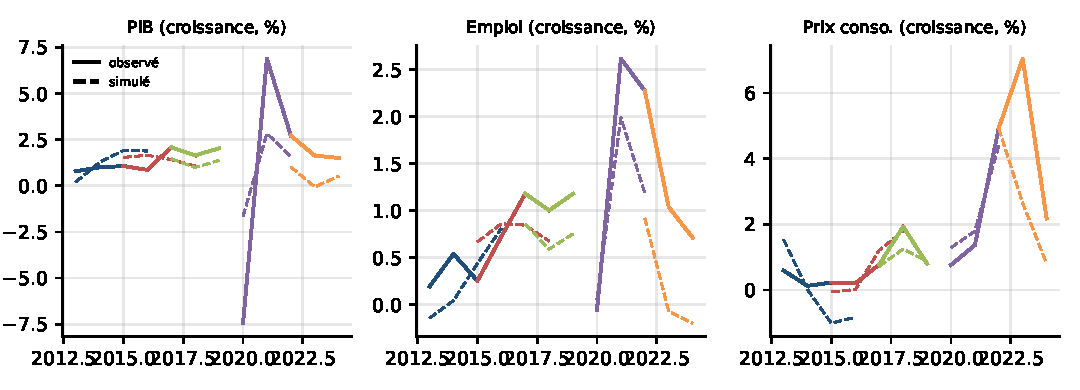
\includegraphics[width=\linewidth]{validation_retro.pdf}
\caption{Simulations hors échantillon : taux de croissance observés (traits pleins) et simulés (tirets), pour
plusieurs origines (estimation arrêtée à l'origine). Source : \code{outputs/validation\_hors\_echantillon.json}.}
\label{fig:validation}
\end{figure}

Le tableau~\ref{tab:retro} résume les tests rétrospectifs du modèle complet. En période calme (2015-2019), le modèle
reproduit la croissance, l'emploi, les prix et le solde public à moins de 1,5~\% ou 0,5 point près sur cinq ans. Il
prévoit mieux qu'un prolongement naïf l'investissement, les importations, l'emploi et les prix, \textbf{mais pas la
croissance du PIB} (erreur quadratique 0,64 point contre 0,50 pour la règle naïve sur 2015-2018). Il échoue sur
2022-2024 pour des raisons identifiées : la productivité a stagné (rétention de main-d'œuvre), les prix de l'énergie et
les marges ont suivi des dynamiques que le modèle ne représente pas.

\begin{table}[htbp]
\centering\small
\caption{Erreur de niveau du modèle complet en fin de période de rétrosimulation (simulé $-$ observé).}
\label{tab:retro}
\begin{tabular}{@{}lrr@{}}
\toprule
Variable & 2015-2019 (base 2014) & 2023-2024 (base 2022) \\
\midrule
PIB en volume & $-$1,0~\% (v0.6) & $-$3,5~\% \\
Investissement & $-$4,9~\% (v0.6) & $-$3,8~\% \\
Emploi & 0,0~\% & $-$0,6~\% \\
Prix à la consommation & +0,5~\% & $-$2,9~\% \\
Revenu disponible brut & +0,1~\% & $-$7,9~\% \\
Dette publique (points de PIB) & +0,4 & +2,0 \\
\bottomrule
\end{tabular}
\end{table}

\section{Sensibilité et robustesse}

La contre-expertise v0.6 a soumis le modèle à des sensibilités univariées sur 22 facteurs, à un criblage de Morris
(138 simulations par scénario) et à 50 tirages conjoints des coefficients estimés. Ses enseignements, qui conditionnent
la lecture de tout ce rapport, sont les suivants.
\begin{enumerate}
\item \textbf{Le facteur décisif n'est pas un coefficient estimé mais une hypothèse de bouclage} : la vitesse de la
fermeture d'offre $\rho$ (section~\ref{sec:fermeture}). Sa plage plausible (0 à 0,4) couvre une vision keynésienne
(la demande détermine durablement l'activité) et une vision classique (l'offre la détermine dès le moyen terme).
\item Les effets de court terme (1-2 ans) sont plus robustes que ceux de cinq ans et au-delà.
\item Le signe de l'effet d'une mesure sur le \textbf{solde public} est presque toujours robuste ; l'effet sur le
\textbf{ratio de dette} l'est beaucoup moins, car il dépend du niveau des prix (dénominateur), lui-même dépendant de la
courbe de Phillips et de l'indexation des salaires, deux paramètres mal identifiés.
\item Les réformes de l'âge de départ sont les mesures les plus incertaines : leur effet sur le PIB dépend de la manière
dont l'économie absorbe un supplément (ou une baisse) d'offre de travail.
\item Une dépense publique de 1 point de PIB a un multiplicateur de 1,26 la première année, 0,58 à cinq ans ; sans
fermeture d'offre 1,25 ; avec une fermeture forte, 0,13.
\end{enumerate}

\section{Ce que le modèle ne représente pas}
\label{sec:audit-manques}

\begin{limites}[Inventaire des faiblesses connues]
\begin{itemize}
\item \textbf{Bouclage de moyen terme non estimé} (fermeture d'offre) : premier facteur d'incertitude.
\item \textbf{Pas de bilans financiers} : pas d'effet de richesse, de patrimoine, de crédit ni de stabilité financière ;
une épargne placée à l'étranger ou en actifs existants n'est pas suivie.
\item \textbf{Pas d'anticipations} : pas d'effet de confiance, d'épargne de précaution liée aux déficits, ni d'effets
annoncés ; les écarts commencent en 2028.
\item \textbf{Emploi et salaires agrégés} : pas de distinction par qualification ; effet du SMIC et des allègements
ciblés mal représenté ; automatisation réduite à la substitution capital-travail.
\item \textbf{Dépenses publiques indistinctes} : santé, éducation, défense, recherche, fonctionnement ont le même effet ;
pas d'effet de l'éducation ou de la recherche sur la productivité ; seul l'investissement public améliore le potentiel.
\item \textbf{Énergie en valeur seulement} : pas de flux physiques, pas de substitution, pas d'émissions.
\item \textbf{Réindustrialisation exogène} : le modèle chiffre les conséquences d'un objectif de relocalisation, pas les
moyens de l'atteindre (aides, compétitivité, qualifications).
\item \textbf{Microsimulation statique, partielle en haut de distribution} : le dernier décile, et surtout le dernier
centile, sont mal représentés : une hausse de 10 points du taux de la tranche supérieure de l'IR rapporte
statiquement 1,7\md{} dans la microsimulation, montant probablement sous-estimé, puis 0,3\md{} seulement après les
réactions d'optimisation et de mobilité de M13 (de +1,0\md{} à $-$1,2\md{} selon l'élasticité retenue) ; les niveaux
de pauvreté et d'inégalités diffèrent de ceux de l'Insee.
\item \textbf{Retraites simplifiées} : pas de régimes, durée d'assurance, décote, réversion.
\item \textbf{Solde extérieur en niveau non fiable} ; RDB sous-estimé en 2023-2024.
\item \textbf{Dette à très long terme} : l'hypothèse d'un taux de 4,89~\% maintenu vingt ans sans réaction de
politique économique produit une dérive explosive de la référence (308~\% du PIB en 2047). Les niveaux de dette au-delà
de 2037 sont illustratifs ; seuls les \emph{écarts} entre scénarios sont interprétés, et avec prudence.
\end{itemize}
\end{limites}


\part{Comprendre les mécanismes par la simulation}
\chapter{La situation de référence}
\label{ch:reference}

Toutes les expériences de ce rapport comparent un avenir « avec mesure » à un avenir « sans mesure ». Ce second
avenir, la \emph{trajectoire de référence à politique inchangée}, est construit en trois temps (fichier
\code{src/m8\_reference.py}) :
\begin{enumerate}
\item \textbf{2023-2025} : le modèle reproduit les comptes observés (Insee, comptes annuels publiés en mai 2026) grâce à
des termes de calage ajoutés aux équations ;
\item \textbf{2026-2031} : la croissance, le chômage et l'inflation suivent les projections du FMI (octobre 2026) ; les
finances publiques sont calculées par le modèle, sans les mesures de redressement que le FMI suppose ;
\item \textbf{après 2031} : productivité par tête +0,7~\% par an et chômage convergeant vers 7~\% (hypothèses centrales
du COR), taux de l'OAT maintenu à 4,89~\%, consommation publique en volume +1,3~\% par an.
\end{enumerate}
Ce n'est pas une prévision : c'est un point de comparaison commun, qui contient ses propres incertitudes. En
particulier, une trajectoire « sans aucune mesure nouvelle pendant vingt ans » n'est pas réaliste ; elle sert à mesurer
l'ampleur des problèmes à résoudre.

\section{Le modèle face aux statistiques observées}

Le tableau~\ref{tab:reference} confronte les grandeurs du modèle aux statistiques publiées. Pour les comptes
nationaux 2023-2025, la concordance est forte \emph{par construction} (calage) : elle vérifie la cohérence comptable,
pas la capacité prédictive. Pour les indicateurs qui ne sont pas calés (niveau de vie, pauvreté, solde extérieur,
pouvoir d'achat), les écarts sont importants et doivent être lus comme des limites du modèle.

\begin{small}
\begin{longtable}{@{}p{4.6cm}rrp{5.2cm}@{}}
\caption{Situation de référence : modèle et statistiques observées (2025 sauf mention).}\label{tab:reference}\\
\toprule
Indicateur & Modèle & Observé & Source de l'observé ; commentaire \\
\midrule\endfirsthead
\toprule Indicateur & Modèle & Observé & Source ; commentaire \\ \midrule\endhead
\bottomrule\endfoot
\multicolumn{4}{@{}l}{\textit{Activité}} \\
PIB en valeur (Md€) & 2\,991 & 2\,991,1 & Insee, comptes de la Nation 2025 (juin 2026) ; calé \\
Croissance du PIB en volume (\%) & 0,81 & 0,8 & idem ; 2024 : 1,51 contre 1,5 \\
PIB par habitant (€) & 43\,370 & 43\,370 & PIB / population moyenne (M1 : 68,97 M) \\
Productivité par tête (\%) & +0,66 & -- & PIB en volume / emploi ; non publié directement \\
Emploi (millions) & 30,64 & calé & Comptes nationaux (Eurostat) \\
Chômage BIT (\%) & 7,44 & 7,7 & Insee, enquête Emploi, France hors Mayotte ; le modèle utilise la série France métropolitaine (moyenne 2025 : 7,5) \\
\multicolumn{4}{@{}l}{\textit{Revenus et demande des ménages}} \\
Salaire moyen par tête (\%) & +2,1 & -- & calé sur les comptes de branche \\
Revenu disponible brut (Md€) & 1\,906 & -- & calé en 2023-2025 \\
Pouvoir d'achat du RDB (\%) & +1,5 & $-$0,7 par UC & Insee Première 2105 ; \textbf{écart} : chute des dividendes reçus en 2025 non captée \\
Consommation en volume (\%) & +0,61 & +0,4 & Insee Première 2105 \\
Taux d'épargne (\% du RDB) & 17,86 & 17,8 & Insee, comptes trimestriels (T1 2026) \\
Investissement en volume (\%) & +0,48 & +0,5 & Insee Première 2105 \\
\multicolumn{4}{@{}l}{\textit{Niveau de vie (microsimulation, revenus 2024)}} \\
Niveau de vie médian (€/UC/an) & 22\,179 & 26\,740 & Insee Première 2117 (2024) ; \textbf{non comparable} : revenus non imposables omis \\
Taux de pauvreté à 60~\% (\%) & 17,3 & 15,4 & idem ; seuil 1\,337~€/mois \\
Indice de Gini & 0,349 & 0,30 & idem ; inégalités surestimées \\
Rapport interdécile D9/D1 & 4,10 & 3,5 & idem \\
\multicolumn{4}{@{}l}{\textit{Échanges extérieurs et énergie}} \\
Solde courant (\% du PIB) & +2,9 & $-$0,4 & Banque de France, balance des paiements 2025 ($-$11,6\md) ; \textbf{niveau non fiable} \\
Solde des biens (Md€) & -- & $-$60,1 & idem ; dont énergie $-$42,4 \\
Indépendance énergétique (\%) & -- & 62,7 & SDES, bilan provisoire 2025 ; non représentée en quantités \\
\multicolumn{4}{@{}l}{\textit{Finances publiques}} \\
Dépenses publiques (\% du PIB) & 57,3 & 57,2 & Insee, comptes des APU 2025 (mars 2026) ; calé \\
Recettes publiques (\% du PIB) & 52,2 & 52,1 & idem \\
Solde public (\% du PIB) & $-$5,07 & $-$5,1 & idem \\
Dette publique (\% du PIB) & 115,7 & 115,6 & idem (115,7 dans la version de mai 2026) \\
Charge d'intérêts (\% du PIB) & 2,47 & -- & calé sur les comptes \\
Prestations sociales en espèces (Md€) & 555 & calé & comptes nationaux (D62) \\
Pensions de droit direct (\% du PIB) & 13,5 & -- & M9 \\
\end{longtable}
\end{small}

\begin{encadre}{Encadré 4.1 — Pourquoi le niveau de vie du modèle diffère de celui de l'Insee}
L'Insee mesure le niveau de vie à partir de l'enquête Revenus fiscaux et sociaux, qui apparie les déclarations de
revenus et les prestations effectivement versées. Le modèle reconstitue les revenus d'un échantillon de ménages réels
à partir de distributions publiées : il ne voit ni les revenus exonérés (une partie des revenus du patrimoine, les
heures supplémentaires défiscalisées réintégrées imparfaitement), ni les prestations non simulées (allocations de
rentrée, prestations d'invalidité…). Le niveau de vie médian est donc trop bas de 17~\% et la dispersion trop forte.
En revanche, quand on compare deux législations sur \emph{le même échantillon}, ces erreurs se compensent en grande
partie : c'est pourquoi le rapport n'utilise la microsimulation que pour des \textbf{variations} (effet d'une mesure sur
le taux de pauvreté au seuil fixe, variation de l'indice de Gini, gains et pertes par décile).
\end{encadre}

\section{La trajectoire de référence jusqu'en 2047}

\begin{figure}[htbp]
\centering
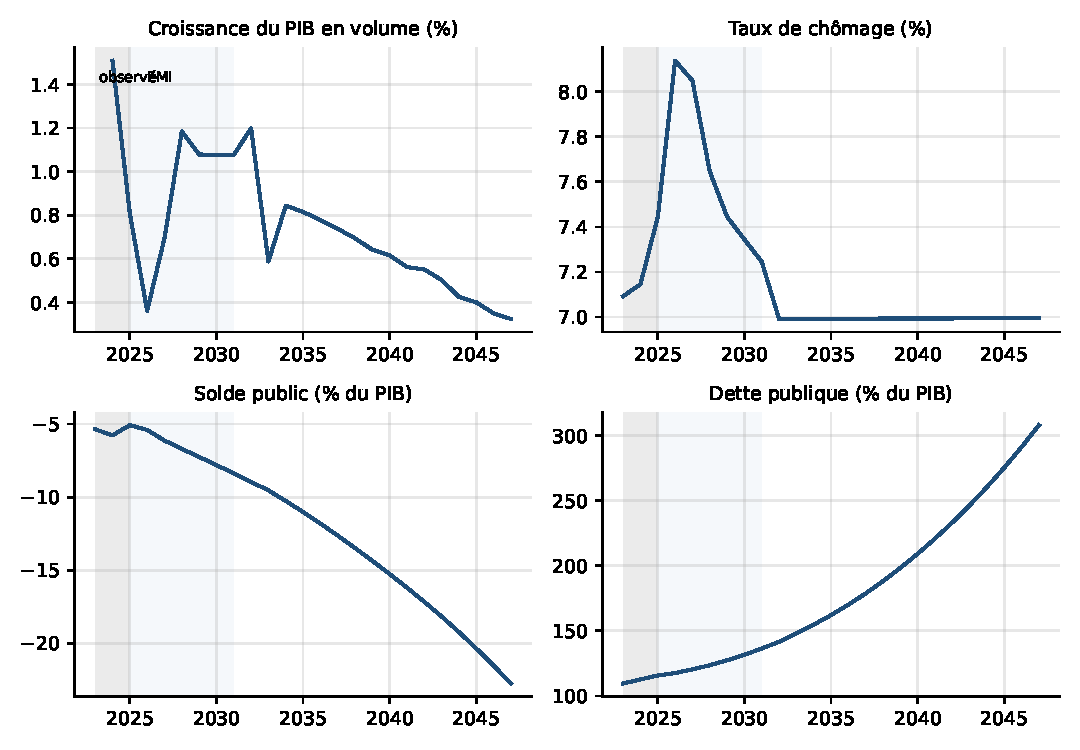
\includegraphics[width=\linewidth]{reference.pdf}
\caption{Trajectoire de référence à politique inchangée. Zone grise : années observées et reproduites ; zone bleutée :
projections calées sur le FMI ; au-delà, hypothèses du COR et du modèle.}
\label{fig:reference}
\end{figure}

\begin{table}[htbp]
\centering\small
\caption{Principaux indicateurs de la trajectoire de référence.}
\label{tab:refproj}
\begin{tabular}{@{}lrrrrrr@{}}
\toprule
 & 2025 & 2026 & 2030 & 2032 & 2037 & 2047 \\
\midrule
Croissance du PIB (\%) & 0,81 & 0,36 & 1,08 & 1,20 & 0,74 & 0,32 \\
Chômage (\%, métropole) & 7,44 & 8,14 & 7,34 & 6,99 & 6,99 & 7,00 \\
Inflation (\%) & 0,83 & 2,37 & 1,88 & 1,78 & 1,78 & 1,76 \\
Taux d'épargne (\%) & 17,9 & 17,6 & 16,0 & 15,5 & 15,5 & 15,5 \\
Solde public (\% du PIB) & $-$5,1 & $-$5,4 & $-$7,8 & $-$9,0 & $-$12,6 & $-$22,8 \\
Dette publique (\% du PIB) & 115,7 & 117,6 & 131,5 & 141,6 & 178,8 & 308,2 \\
Charge d'intérêts (\% du PIB) & 2,5 & 2,9 & 4,4 & 5,1 & 7,2 & 13,6 \\
Pensions de droit direct (\% du PIB) & 13,5 & 13,3 & 14,0 & 14,2 & 14,7 & 15,7 \\
Industrie manufacturière (\% du PIB) & 9,6 & 9,5 & 9,0 & 8,7 & 8,4 & 9,2 \\
Emploi (millions) & 30,64 & 30,50 & 31,23 & 31,53 & 31,67 & 31,25 \\
Population active (millions) & 33,10 & 33,21 & 33,71 & 33,90 & 34,05 & 33,60 \\
Plus de 65 ans / 20-64 ans & 0,39 & 0,40 & 0,43 & -- & 0,47 & 0,51 \\
\bottomrule
\end{tabular}
\end{table}

\paragraph{Lecture.} Quatre dynamiques dominent la référence.
\begin{enumerate}
\item \textbf{Une croissance faible et déclinante} : 1,1 à 1,2~\% jusqu'en 2032, puis moins de 0,8~\% par an, puis
0,3~\% en fin de période. Elle résulte de la productivité supposée (+0,7~\% par tête) et du plafonnement puis du recul
de la population active à partir du milieu des années 2030 (vieillissement, fécondité de 1,45). La croissance est donc
d'abord une question de \emph{productivité} et de \emph{nombre d'actifs}.
\item \textbf{Une dérive des finances publiques} : sans mesure, le déficit passe de 5,1 à 9~\% du PIB en 2032. Les
causes, par ordre d'importance : la charge d'intérêts (de 2,5 à 5,1 points de PIB, car la dette émise à 1-2~\% est
progressivement refinancée à près de 5~\%), la hausse des pensions avec le vieillissement, et une dépense publique en
volume qui croît plus vite que l'activité (1,3~\% par an contre 1,1~\%). Au-delà, l'« effet boule de neige » rend la
trajectoire explosive. Le FMI, qui suppose un redressement non encore voté, projette un solde de $-$3,9~\% et une dette
de 124~\% en 2031 : l'écart, environ 4 points de PIB, mesure l'effort que ce redressement représenterait.
\item \textbf{Un vieillissement qui pèse sur la protection sociale} : 0,39 personne de 65 ans ou plus pour une personne
de 20 à 64 ans en 2025, 0,47 en 2037, 0,51 en 2047 ; les pensions passent de 13,5 à 15,7~\% du PIB.
\item \textbf{Une désindustrialisation tendancielle} : la part de l'industrie manufacturière baisse jusqu'à 8,4~\% en
2037. La remontée de la fin de période est un artefact (prix relatifs de 2022 non chaînés) qu'il ne faut pas
interpréter.
\end{enumerate}

\begin{limites}[Fiabilité de la référence]
Les comptes 2023-2025 sont reproduits \fiab{robuste}. Les projections 2026-2031 reprennent celles du FMI pour la
croissance, le chômage et l'inflation \fiab{conventionnel}. Les finances publiques sont calculées par le modèle : leur
dérive est \fiab{plutôt robuste} dans son sens (taux d'intérêt et démographie), \fiab{fragile} dans son ampleur au-delà
de 2035 (hypothèse de taux constant à 4,89~\%, absence de toute réaction de politique économique). Le solde extérieur
de la référence se dégrade continûment (de +2,9 à $-$7,7~\% du PIB) sous l'effet de la tendance de pénétration des
importations estimée sur 1997-2019 : \fiab{non établi}.
\end{limites}

\chapter{Huit expériences pour isoler les mécanismes}
\label{ch:experiences}

\section{Protocole commun}

Chaque expérience modifie un seul levier, à partir du 1\textsuperscript{er} janvier 2028, et le maintient jusqu'en 2047.
Le modèle complet est utilisé : microsimulation des ménages quand la mesure s'y prête, réactions des hauts revenus
(M13, valeurs centrales), hétérogénéité des propensions (M14), retraites (M9) et rétroactions européennes (M11 : taux
de la BCE, taux longs, prime de risque, demande des partenaires). Les montants sont exprimés en euros de 2025 et
indexés sur le PIB nominal. Les résultats sont des \textbf{écarts à la trajectoire de référence} : un « PIB $-$0,2~\% »
signifie un PIB inférieur de 0,2~\% à ce qu'il aurait été sans la mesure, pas une récession. Soixante simulations ont
été réalisées (script \code{rapport/simulations.py}, résultats dans \code{rapport/resultats/experiences\_*.json}).

Les horizons sont : \textbf{court terme} 2029 (deuxième année), \textbf{moyen terme} 2032 (cinq ans),
\textbf{long terme} 2037 (dix ans), \textbf{très long terme} 2047 (vingt ans). Les effets sur la pauvreté et les
inégalités sont \textbf{statiques} (première année, revenus 2024, au seuil de pauvreté d'avant réforme).

Pour chaque expérience, la présentation suit huit rubriques : situation initiale, modification, mécanismes,
résultats, effets indirects, gagnants et perdants, horizons, conditions d'inversion.

\begin{encadre}{Encadré 5.1 — Comment lire les tableaux d'expériences}
\textbf{$\Delta$solde} : variation du solde public en points de PIB (positif = amélioration). \textbf{PIB} : écart en
\% du PIB en volume. \textbf{Emploi} : écart en milliers de personnes. \textbf{Dette} : écart en points de PIB
(négatif = moins de dette). \textbf{Pauvreté} : variation du taux de pauvreté en points, au seuil fixe, effet statique
(« -- » quand la mesure ne passe pas par la microsimulation). \textbf{RDB réel} : pouvoir d'achat du revenu disponible
brut de l'ensemble des ménages. Les écarts de prix, de RDB réel, de consommation, d'investissement et de commerce
extérieur sont en \%, l'épargne et les recettes en points.
\end{encadre}

% ====================================================================================================
\section{Expérience 1 : augmenter les impôts}
\label{sec:exp1}

\paragraph{Situation initiale.} En 2025, les prélèvements obligatoires représentent environ 52~\% du PIB de recettes
publiques. Le déficit atteint 5,1~\% du PIB et, dans la référence, se dégrade jusqu'à 9~\% en 2032.

\paragraph{Modifications.} Onze hausses de prélèvements, de rendement statique comparable (5 à 11\md{} par an, sauf la
tranche supérieure de l'IR) : impôt sur le revenu (première tranche +2 points ; tranche supérieure +10 points), CSG sur
les revenus d'activité (+1 point), TVA (taux normal +1 point ; taux réduits +2 points), impôt sur la fortune (taux moyen
1~\% au-delà de 1,3\,M€), prélèvement forfaitaire unique (+15 points), impôt sur les sociétés (25,8~\% $\to$ 30,5~\%),
impôts de production (+10\md), cotisations employeurs (+10\md), droits de succession (+50~\%), taxe carbone (+50~€ par
tonne).

\paragraph{Mécanismes.} Toute hausse d'impôt prélève du pouvoir d'achat ou des profits. Ce qui distingue les impôts,
c'est \emph{qui} paie et \emph{par quel canal} l'activité est touchée :
\begin{itemize}
\item \textbf{impôts sur le revenu des ménages (IR, CSG)} : baisse du revenu disponible $\to$ consommation $\to$
production et emploi ; l'effet dépend de la propension à consommer des ménages touchés (M14) ;
\item \textbf{impôts sur la consommation (TVA, taxe carbone)} : hausse des prix $\to$ baisse du pouvoir d'achat de
\emph{tous} les revenus, y compris les prestations et les pensions (indexées avec retard) ; les salaires suivent
partiellement les prix, ce qui renchérit le coût du travail ;
\item \textbf{impôts sur le capital et le patrimoine (ISF, PFU, successions)} : touchent des ménages à faible propension
à consommer ; leur rendement est réduit par les réactions d'optimisation et de départ (M13) ;
\item \textbf{impôts sur les entreprises (IS, production, cotisations)} : l'IS passe par le coût du capital
(investissement) ; les impôts de production et les cotisations par les coûts (prix et emploi).
\end{itemize}

\begin{table}[htbp]
\centering\scriptsize
\caption{Expérience 1 — Rendement statique et amélioration effective du solde public. « Conservé » : part du rendement
net des réactions comportementales effectivement retrouvée dans le solde en 2029, après les effets sur l'activité.}
\label{tab:rendement}
\tabfit{../tableaux/tab_rendement}
\end{table}

\paragraph{Résultats.} (Tableaux~\ref{tab:rendement}, \ref{tab:impots} et \ref{tab:impotsd}.)
\begin{enumerate}
\item \textbf{Toutes les hausses d'impôts testées améliorent le solde public}, à tous les horizons, dans le scénario
central. Mais une partie du rendement attendu disparaît : seuls \textbf{58~\% à 79~\%} du rendement net sont retrouvés
dans le solde en 2029 pour les impôts sur les ménages et sur le travail. La raison est que la baisse d'activité réduit
les autres recettes (cotisations, TVA, impôt sur le revenu) et augmente certaines dépenses (allocations chômage).
\item La perte de recettes induite est la plus forte pour la \textbf{taxe carbone} (42~\% du rendement perdu en 2029),
qui pèse sur les prix et sur tous les revenus, et pour la \textbf{CSG} et l'\textbf{IR de la première tranche} (33~\%),
qui touchent des ménages à propension à consommer moyenne. Elle est plus faible pour la \textbf{TVA} (25~\%), dont une
partie de la charge porte sur le contenu importé de la consommation, et pour les \textbf{impôts sur le patrimoine}
(21~\% du rendement net), qui touchent des ménages qui épargnent davantage.
\item Les \textbf{impôts de production} et les \textbf{droits de succession} paraissent « gratuits » (plus de 100~\%
retrouvé) : c'est une \textbf{conséquence des limites du modèle}, qui ne représente ni l'effet des impôts de production
sur l'investissement et la localisation des activités, ni le comportement des héritiers ; l'impôt de production relève
en outre les prix, donc les recettes nominales. Ces deux résultats sont \fiab{non établis}.
\item L'\textbf{IS} rapporte durablement (+0,50 point de PIB de solde en 2032, dette $-$14,9 points en 2047) avec un
effet faible sur le PIB ($-$0,07~\% en 2032) car l'élasticité de l'investissement au coût du capital est faible
($-$0,18). Ce résultat est \fiab{fragile} : il ignore la localisation des profits et des sièges, qui est le principal
canal identifié par la littérature récente pour un pays ouvert.
\item La \textbf{tranche supérieure de l'IR} (+10 points) rapporte 1,7\md{} statiques mais seulement 0,3\md{} après
les réactions des contribuables (valeur centrale) ; avec l'élasticité haute (0,4), le rendement devient
\textbf{négatif} ($-$1,2\md) : c'est le seul cas, dans le modèle, où une hausse d'impôt réduirait les recettes. Le
nombre de départs de foyers serait de l'ordre de 5\,000 à 13\,000 (indicatif).
\end{enumerate}

\begin{table}[htbp]
\centering\scriptsize
\caption{Expérience 1 — Effets macroéconomiques et sociaux des hausses d'impôts.}
\label{tab:impots}
\tabfit{../tableaux/tab_impots}
\end{table}

\begin{table}[htbp]
\centering\scriptsize
\caption{Expérience 1 — Effets en 2030 sur les comptes des agents.}
\label{tab:impotsd}
\tabfit{../tableaux/tabd_impots}
\end{table}

\begin{figure}[htbp]
\centering
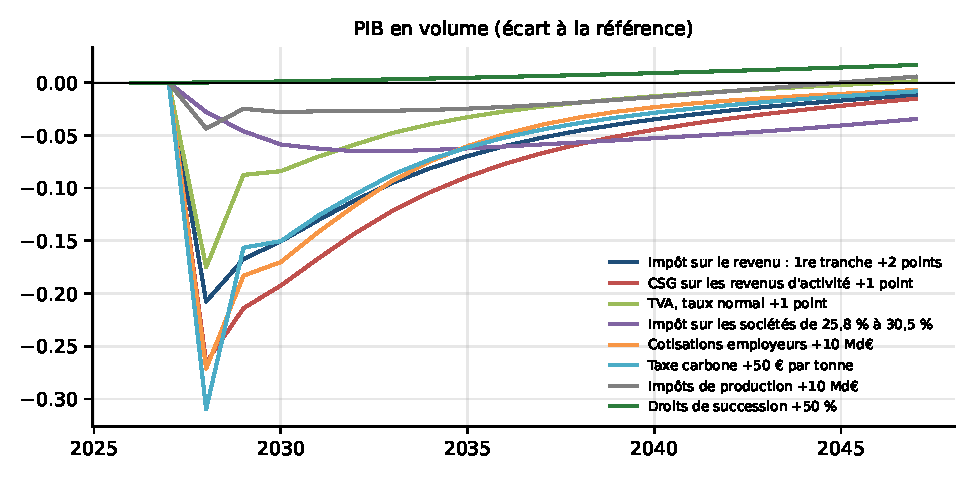
\includegraphics[width=0.95\linewidth]{pib_impots.pdf}\\
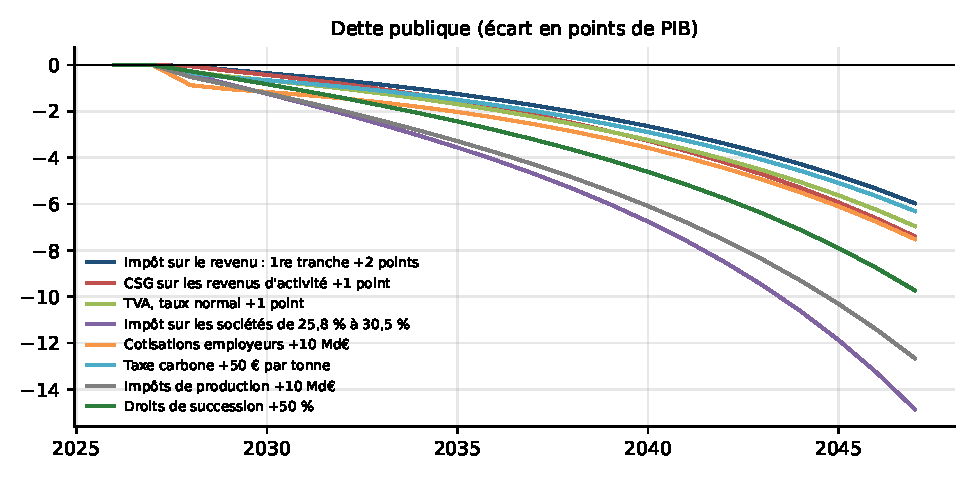
\includegraphics[width=0.95\linewidth]{dette_impots.pdf}
\caption{Expérience 1 — Trajectoires du PIB et de la dette (écarts à la référence).}
\label{fig:impots}
\end{figure}

\paragraph{Effets indirects.} \emph{Épargne} : les ménages amortissent une partie du choc en épargnant moins (taux
d'épargne $-$0,06 à $-$0,09 point pour l'IR, la CSG, l'ISF et le PFU). \emph{Investissement} : il recule avec la
demande ($-$0,2 à $-$0,3~\% pour les impôts sur les ménages) et davantage avec l'IS ($-$0,44~\%). \emph{Prix} : la
TVA et la taxe carbone relèvent les prix (+0,42~\% et +0,74~\%), les impôts sur le revenu les baissent légèrement à
moyen terme (moindre demande). \emph{Commerce extérieur} : les importations baissent avec la demande ; le solde
extérieur s'améliore légèrement. \emph{Dette} : outre le solde, le niveau des prix joue sur le ratio ; les impôts sur la
consommation, qui élèvent les prix, réduisent un peu plus le ratio de dette que les impôts sur le revenu.

\begin{figure}[htbp]
\centering
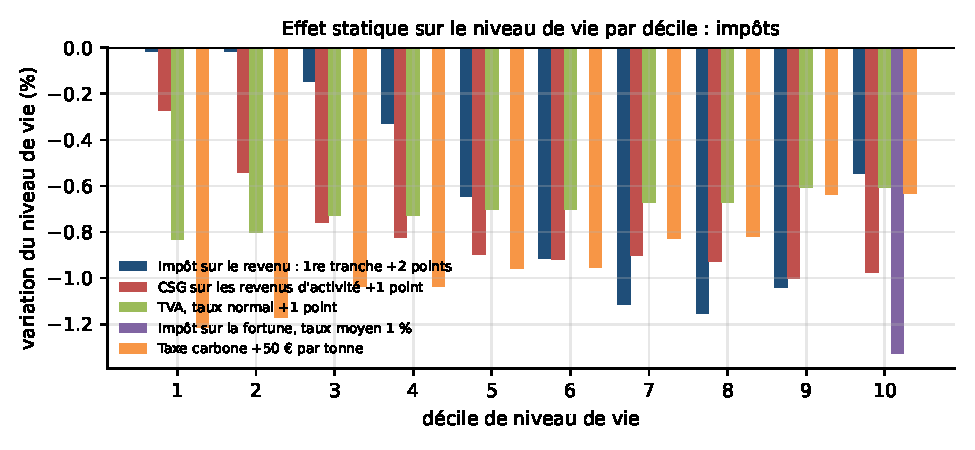
\includegraphics[width=0.9\linewidth]{distribution_impots.pdf}
\caption{Expérience 1 — Variation statique du niveau de vie par décile (microsimulation).}
\label{fig:distimpots}
\end{figure}

\paragraph{Gagnants et perdants.} (Figure~\ref{fig:distimpots}.) Les impôts sur la consommation sont
\textbf{dégressifs} par rapport au niveau de vie : la TVA retire 0,83~\% du niveau de vie du premier décile et 0,61~\% du
dernier ; la taxe carbone 1,21~\% contre 0,63~\%. Ils augmentent la pauvreté (+0,30 et +0,45 point au seuil fixe). La
CSG sur les revenus d'activité est à peu près proportionnelle au-dessus du deuxième décile (0,8 à 1~\%) et épargne en
partie les plus modestes ; elle augmente aussi la pauvreté (+0,38 point) parce qu'elle touche des travailleurs proches du
seuil. La première tranche de l'IR touche les déciles 5 à 9 ($-$0,9 à $-$1,2~\%). L'ISF et le PFU ne touchent que le
dernier décile ($-$1,3~\%) et réduisent l'indice de Gini de 0,28 point. \emph{Note} : la variation de $-$1,7~\% du premier
décile pour la tranche supérieure de l'IR est un artefact de la mesure approchée du niveau de vie (quelques foyers à
revenu fiscal élevé mais à niveau de vie calculé faible) et ne doit pas être interprétée.

\paragraph{Horizons.} L'effet sur le PIB est maximal la première année ($-$0,1 à $-$0,3~\% pour 8 à 11\md) puis
s'estompe : il est divisé par deux en cinq ans et presque nul en vingt ans, car la fermeture d'offre ramène le chômage
vers son niveau structurel. L'effet sur la dette, lui, s'accumule : $-$1,7 à $-$2,6 points en 2037, $-$6 à $-$7,5 points en
2047 pour 8 à 11\md, grâce aux intérêts économisés.

\paragraph{Conditions d'inversion.} Le solde pourrait se dégrader après une hausse d'impôt si (1) l'assiette réagit
fortement (taux marginaux élevés, contribuables mobiles : cas de la tranche supérieure de l'IR avec l'élasticité haute) ;
(2) la hausse provoque une récession durable, ce qui suppose une fermeture d'offre nulle ($\rho = 0$) \emph{et} un
multiplicateur supérieur à 1/(taux de prélèvement marginal), soit environ 2, hors de la plage du modèle ; (3) pour
l'IS, si les profits se délocalisent, ce que le modèle ne représente pas. \fiab{robuste} pour le signe de l'effet sur
le solde ; \fiab{plutôt robuste} pour l'ordre de grandeur de la perte d'activité de court terme.

\begin{resultat}
Une hausse d'impôt réduit le déficit, mais d'environ un quart à un tiers de moins que son rendement statique la
première année, à cause de l'activité perdue. Le coût en activité par euro de déficit réduit est le plus faible pour les
impôts sur le patrimoine et la TVA, le plus élevé pour la taxe carbone, les cotisations, la CSG et l'IR des classes
moyennes. Les impôts sur la consommation sont les plus défavorables aux ménages modestes.
\end{resultat}

% ====================================================================================================
\section{Expérience 2 : augmenter les salaires}
\label{sec:exp2}

\paragraph{Situation initiale.} Le salaire moyen par tête progresse d'environ 2~\% par an dans la référence ; la part des
salaires dans la valeur ajoutée est à sa norme de 2022.

\paragraph{Modifications.} Hausse générale ponctuelle de 2~\% et de 5~\% en 2028 ; « coup de pouce » au SMIC de 5~\% et
10~\% ; point d'indice de la fonction publique +3~\%.

\paragraph{Mécanismes.} Une hausse de salaire est à la fois un \emph{revenu} pour les ménages et un \emph{coût} pour les
entreprises. Dans le modèle :
\begin{enumerate}
\item le revenu des salariés augmente $\to$ consommation $\uparrow$ (effet de demande) ;
\item le coût salarial unitaire augmente $\to$ les entreprises relèvent leurs prix (0,67 la première année, tout à long
terme) $\to$ le pouvoir d'achat est en partie repris par l'inflation ;
\item le coût réel du travail augmente tant que les prix n'ont pas rattrapé $\to$ substitution du capital au travail
($\sigma = 0{,}4$) $\to$ emploi $\downarrow$ ;
\item les prix à l'exportation augmentent $\to$ perte de compétitivité-prix $\to$ exportations $\downarrow$ ;
\item les prestations sont indexées sur les prix avec retard ; les prestations sous condition de ressources (prime
d'activité, aides au logement) baissent quand le salaire augmente (effet de seuil, voir plus bas) ;
\item les recettes publiques augmentent avec la masse salariale et les prix (cotisations, TVA) ; pour le SMIC, les
allègements de cotisations indexés sur le SMIC et la masse salariale publique coûtent 0,66\md{} par point.
\end{enumerate}

\begin{table}[htbp]
\centering\scriptsize
\caption{Expérience 2 — Effets des hausses de salaires.}
\label{tab:salaires}
\tabfit{../tableaux/tab_salaires}\\[4pt]
\tabfit{../tableaux/tabd_salaires}
\end{table}

\begin{figure}[htbp]
\centering
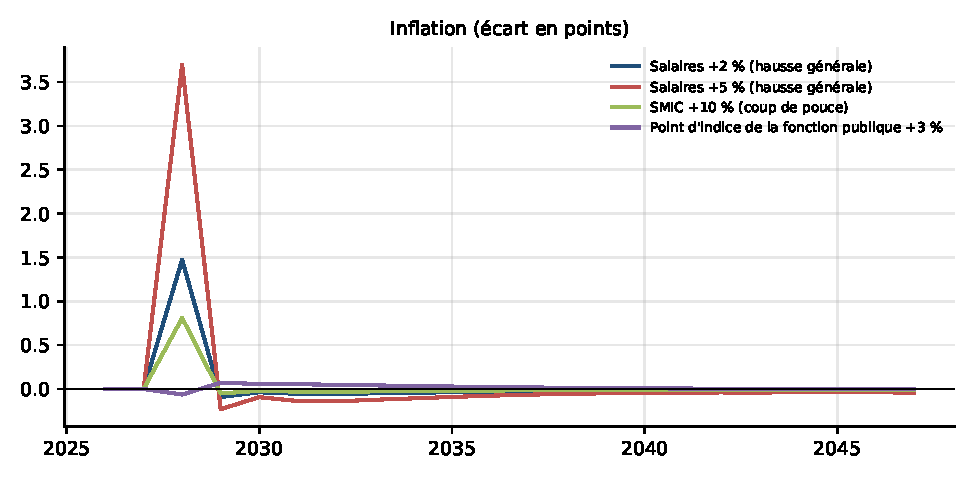
\includegraphics[width=0.48\linewidth]{inflation_salaires.pdf}\hfill
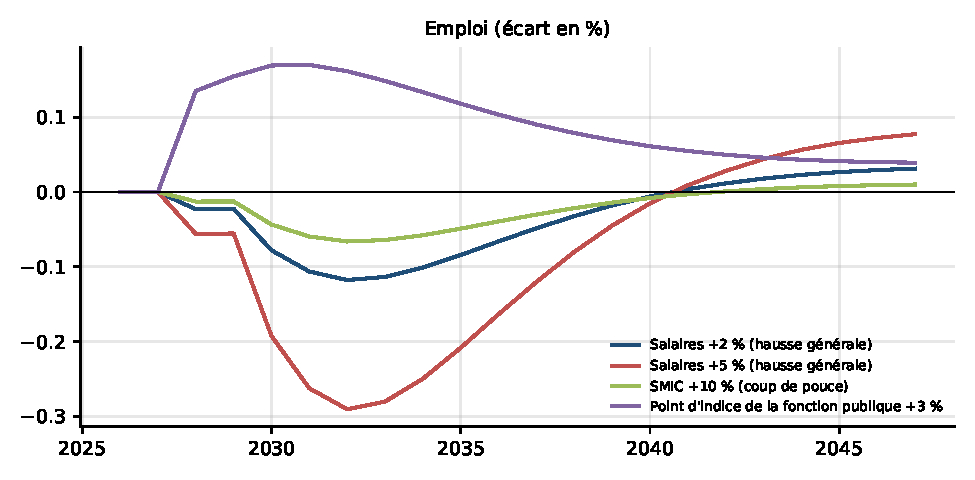
\includegraphics[width=0.48\linewidth]{emploi_salaires.pdf}
\caption{Expérience 2 — Inflation et emploi après une hausse de salaires.}
\label{fig:salaires}
\end{figure}

\paragraph{Résultats.} Une hausse générale de 2~\% en 2028 augmente le salaire moyen de 2,4~\% en 2030 (diffusion par
l'indexation), les prix de 1,3~\%, le pouvoir d'achat du revenu disponible de 0,56~\% et la consommation de 0,49~\%.
Les exportations reculent de 0,6~\%. L'emploi baisse peu la première année ($-$7\,000) puis davantage
($-$37\,000 en 2032), à mesure que la substitution capital-travail joue. Au total, le PIB est presque inchangé
(+0,02~\% en 2032) : \textbf{les effets de demande et de coût se compensent}. Le solde public s'améliore (+0,25 point en
2032) et la dette baisse de 3 à 4 points, surtout parce que l'inflation gonfle le PIB nominal et les recettes alors que
les prestations ne sont revalorisées qu'avec un an de retard. Les résultats pour +5~\% sont proportionnels.

Le \textbf{point d'indice} (+3~\%) agit comme une dépense publique : pouvoir d'achat +0,76~\%, PIB +0,22~\% en 2029,
emploi +48\,000, mais solde $-$0,25 point et dette +2,1 points en 2037.

Le \textbf{coup de pouce au SMIC} de 10~\% (diffusion supposée de 11~\% à la masse salariale) a des effets
macroéconomiques faibles : pouvoir d'achat +0,30~\%, emploi $-$21\,000 en 2032, solde $-$0,13 point (coût des allègements
indexés). \textbf{Ce résultat sous-estime probablement les pertes d'emploi peu qualifié} : le modèle n'a qu'un salaire
moyen et une élasticité de l'emploi au coût du travail commune à tous les niveaux de qualification.

\paragraph{Une hausse de salaire peut-elle augmenter la pauvreté ? Vérification par les effets de seuil.} La
microsimulation ne fait pas varier les salaires des ménages (elle est statique). Pour répondre à la question sans
présumer la réponse, le revenu disponible de trois ménages types a été calculé avec OpenFisca pour des salaires
de 0 à 2,5 SMIC (script \code{rapport/seuils\_salaires.py}, législation 2024, locataires en zone 2).

\begin{figure}[htbp]
\centering
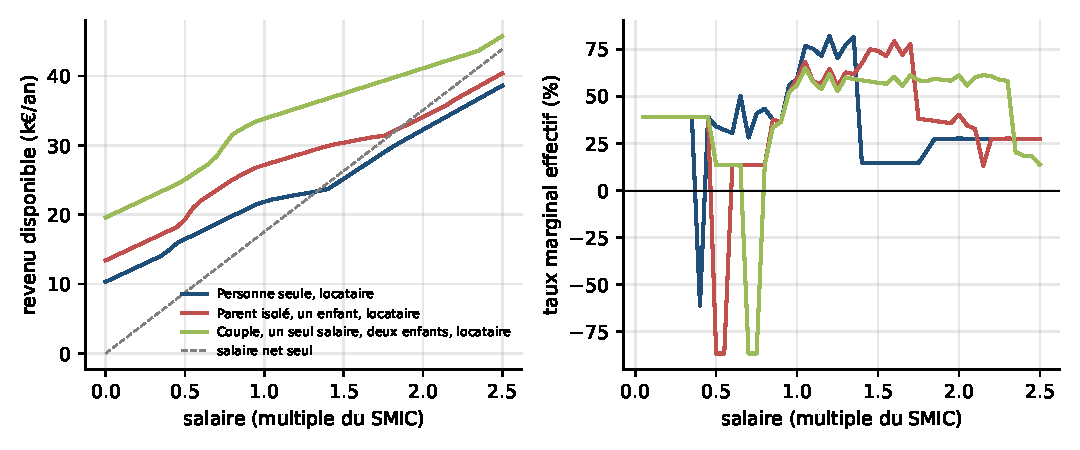
\includegraphics[width=\linewidth]{seuils_salaires.pdf}
\caption{Revenu disponible (gauche) et taux marginal effectif de prélèvement d'une hausse de salaire de 2~\% (droite)
selon le salaire, pour trois ménages types. Salaire exprimé en multiple du SMIC net imposable annuel (17\,900~€).
Revenu disponible = salaire net + RSA + prime d'activité + allocations familiales + aides au logement $-$ impôt sur le
revenu.}
\label{fig:seuils}
\end{figure}

Trois constats (figure~\ref{fig:seuils}) :
\begin{enumerate}
\item \textbf{Le revenu disponible augmente toujours avec le salaire} : il n'existe pas, dans la législation 2024 telle
qu'OpenFisca la calcule, de zone où gagner plus fait perdre du revenu disponible (pas de « trappe » au sens strict).
\item \textbf{Mais le gain est très faible entre 1 et 2 SMIC} : le taux marginal effectif atteint 55 à 82~\% (sortie
progressive de la prime d'activité et des aides au logement, entrée dans l'impôt sur le revenu). Une hausse de salaire
de 2~\% pour une personne seule au SMIC (358~€ de salaire imposable par an) ne lui rapporte que 142~€ ; pour un couple avec deux
enfants et un seul salaire, le taux marginal reste supérieur à 50~\% jusqu'à 2,2 SMIC.
\item Entre 0,3 et 0,8 SMIC, la bonification de la prime d'activité rend le taux marginal \emph{négatif} pour certains
ménages (jusqu'à $-$86~\%) : une hausse de salaire rapporte plus qu'elle-même.
\end{enumerate}

\textbf{Conclusion sur la pauvreté} : dans le modèle, une hausse de salaire \emph{n'augmente pas} la pauvreté par effet
de seuil ; elle la réduit faiblement pour les salariés modestes, car l'essentiel du gain brut est repris par la baisse
des prestations. Elle peut \emph{indirectement} toucher d'autres catégories : (1) les ménages sans revenu d'activité
(retraités, allocataires du RSA, chômeurs) subissent la hausse des prix (+1,3~\% pour +2~\% de salaires) avec un an de
retard de revalorisation ; (2) les salariés dont l'emploi est supprimé (39\,000 en 2032 pour +2~\%) ; (3) pour le SMIC,
les travailleurs peu qualifiés, dont l'emploi est probablement plus sensible au coût du travail que ne le représente
le modèle. L'ampleur de ces effets indirects sur le taux de pauvreté n'est pas mesurable avec la microsimulation
statique : \fiab{non établi}.

\paragraph{Gagnants et perdants.} Gagnants : salariés en emploi (pouvoir d'achat), administrations (inflation).
Perdants : titulaires de revenus fixes ou revalorisés avec retard (pensions, minima sociaux), salariés licenciés,
secteurs exportateurs (marges et parts de marché).

\paragraph{Horizons et inversion.} À court terme, l'effet de demande domine légèrement ; à moyen terme, l'effet de coût
(emploi $-$37\,000 à $-$92\,000 en 2032). Le résultat s'inverserait (PIB nettement négatif) si la substitution
capital-travail était forte ($\sigma = 0{,}7$) ou si les prix ne répercutaient pas les coûts (marges comprimées : emploi
$-$68\,000 pour +2~\%, contre-expertise test 5e) ; il serait plus favorable si la hausse était ciblée sur les bas
salaires des ménages à forte propension à consommer (PIB +0,13~\% en 2032, mais emploi peu qualifié non représenté).
\fiab{plutôt robuste} pour les prix et le pouvoir d'achat ; \fiab{fragile} pour l'emploi.

\begin{resultat}
Une hausse générale des salaires ne crée ni ne détruit beaucoup d'activité dans le modèle : elle redistribue vers les
salariés en emploi, au détriment des revenus fixes et de l'emploi à moyen terme. Les effets de seuil des prestations
réduisent fortement le gain net d'une hausse de salaire entre 1 et 2 SMIC (taux marginaux de 55 à 82~\%) sans créer de
perte nette de revenu disponible.
\end{resultat}

% ====================================================================================================
\section{Expérience 3 : réduire les dépenses publiques}
\label{sec:exp3}

\paragraph{Situation initiale.} Dépenses publiques : 57,3~\% du PIB en 2025, 61,5~\% en 2030 dans la référence (charge
d'intérêts, pensions).

\paragraph{Modifications.} Dix économies d'environ 10\md{} par an (ou équivalent) : 170\,000 emplois publics en moins
(en cinq ans) ; fonctionnement, santé, éducation, défense ($-$10\md{} chacun) ; investissement public ($-$10\md) ;
sous-indexation des pensions d'un point par an ; allocations chômage $-$25~\% ; prestations familiales et logement
$-$10~\% ; transferts monétaires non ciblés $-$0,3 point de PIB.

\begin{table}[htbp]
\centering\scriptsize
\caption{Expérience 3 — Effets des économies de dépenses.}
\label{tab:depenses}
\tabfit{../tableaux/tab_depenses}\\[4pt]
\tabfit{../tableaux/tabd_depenses}
\end{table}

\begin{figure}[htbp]
\centering
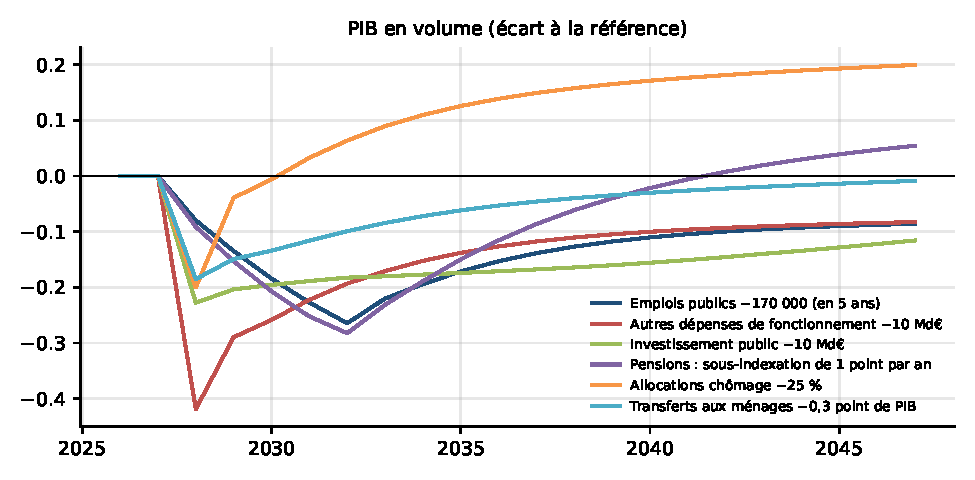
\includegraphics[width=0.95\linewidth]{pib_depenses.pdf}\\
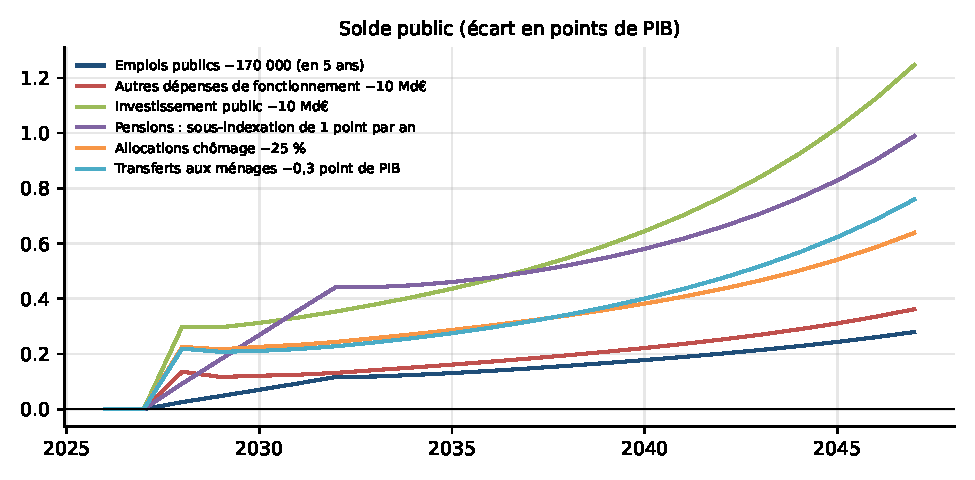
\includegraphics[width=0.95\linewidth]{solde_depenses.pdf}
\caption{Expérience 3 — PIB et solde public après différentes économies de dépenses.}
\label{fig:depenses}
\end{figure}

\paragraph{Mécanismes.} Une économie de dépense publique réduit directement la demande (achats publics, rémunérations)
ou le revenu des ménages (prestations). Deux économies de même montant diffèrent par :
\begin{enumerate}
\item \textbf{le contenu en valeur ajoutée nationale} : une dépense de fonctionnement ou un emploi public est presque
entièrement de la valeur ajoutée française ; une prestation est en partie épargnée et en partie consommée en produits
importés ; un investissement public a un contenu importé élevé (0,23 pour l'investissement contre 0,13 pour la
consommation) ;
\item \textbf{la propension à consommer des bénéficiaires} : réduire les prestations des ménages modestes réduit
davantage la consommation que réduire celles des ménages aisés ;
\item \textbf{l'effet d'offre} : seul l'investissement public améliore la capacité de production à long terme dans le
modèle ;
\item \textbf{les effets sur le marché du travail} : une baisse des allocations chômage réduit, par hypothèse, le
chômage structurel (0,1 point pour 10~\%, hypothèse \preuve{H}).
\end{enumerate}

\paragraph{Résultats.}
\begin{enumerate}
\item \textbf{Fonctionnement, santé, éducation, défense : effets identiques} ($-$0,29~\% de PIB en 2029, $-$83\,000
emplois, +0,13 point de solde en 2032). Ce n'est pas un résultat économique mais une \textbf{limite du modèle} : il ne
distingue pas ces fonctions (section~\ref{sec:depenses}). Il ne mesure ni les conséquences sur la santé, l'éducation ou
la sécurité, ni leurs effets différés sur la productivité.
\item Une économie de fonctionnement de 10\md{} n'améliore le solde que de 3,6 à 4\md{} (0,12-0,13 point de PIB) : la
moitié à deux tiers de l'économie est perdue en recettes (moindre activité) et en dépenses induites (chômage) ; c'est le
\emph{multiplicateur} de la dépense publique, proche de 1 la première année.
\item \textbf{Les économies sur les transferts sont moins coûteuses en activité} : réduire de 0,3 point de PIB
(environ 10\md) les transferts non ciblés coûte $-$0,15~\% de PIB en 2029 pour +0,21 point de solde ; la
sous-indexation des pensions $-$0,15~\% pour +0,18 point (puis +0,44 en 2032 car l'économie s'accumule) ; les
prestations familiales et de logement $-$0,06~\% pour +0,05 point.
\item \textbf{L'investissement public est l'économie la plus coûteuse à long terme} : $-$0,20~\% de PIB en 2029 mais
encore $-$0,12~\% en 2047, car le capital public se dégrade ; elle améliore pourtant fortement le solde (+0,35 point en
2032) car son contenu importé est élevé et elle n'entraîne pas de pertes de recettes importantes à court terme.
\item \textbf{La baisse des allocations chômage} ($-$25~\%) améliore le solde (+0,24 point en 2032) et, par l'hypothèse
d'effet sur le chômage structurel, augmente l'emploi à long terme (+52\,000 en 2037, PIB +0,15~\%). Sans cette
hypothèse \preuve{H}, elle n'aurait que des effets de demande négatifs.
\item La suppression de 170\,000 emplois publics en cinq ans réduit le PIB de 0,26~\% en 2032 (perte de production non
marchande), améliore peu le solde (+0,12 point) et ne réduit la dette que de 1,6 point en 2047.
\end{enumerate}

\begin{figure}[htbp]
\centering
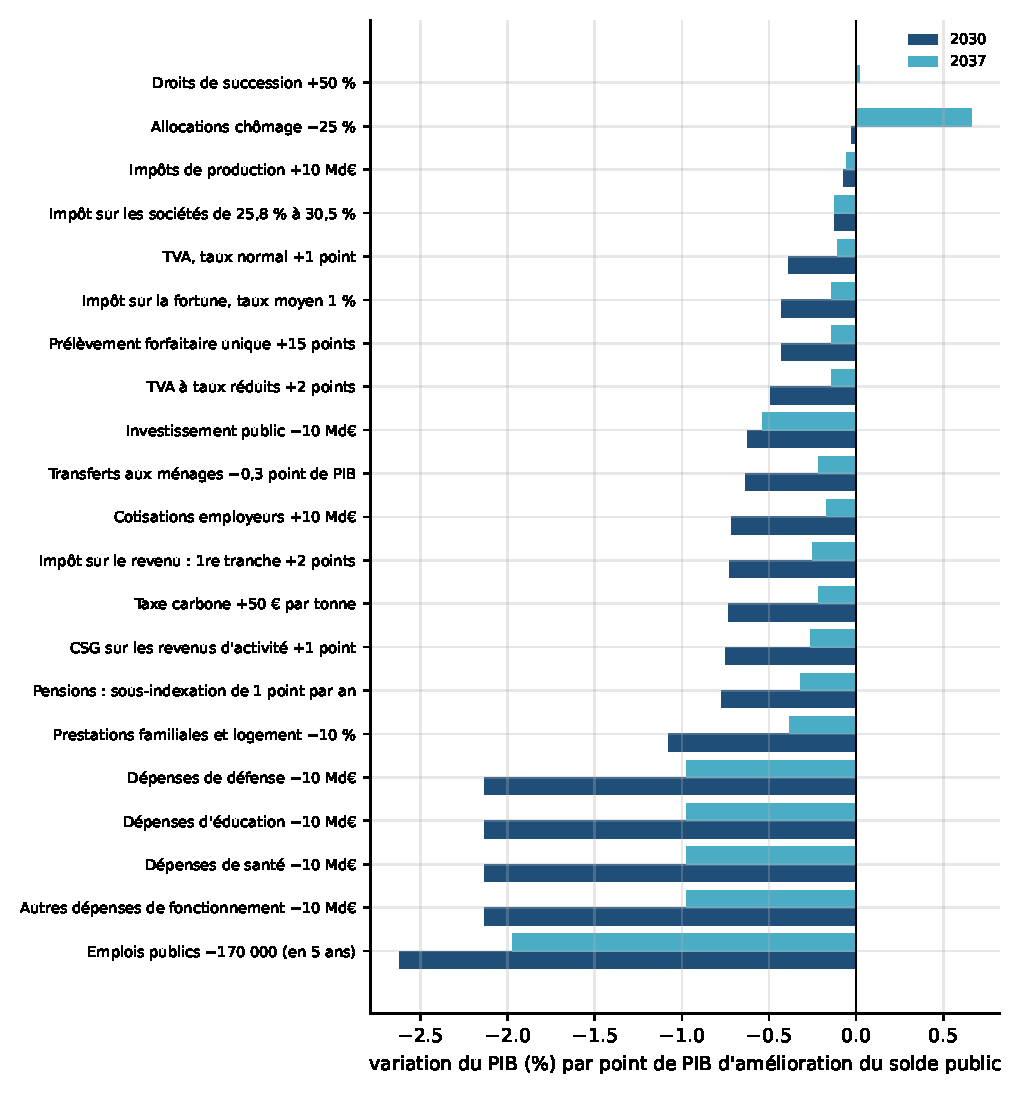
\includegraphics[width=0.9\linewidth]{efficacite_consolidation.pdf}
\caption{Coût en activité d'un point de PIB de solde public amélioré : variation du PIB (en \%) par point de PIB de
solde gagné, en 2030 et 2037. Plus la barre est à gauche, plus la mesure coûte en activité par euro de déficit réduit.}
\label{fig:efficacite}
\end{figure}

\paragraph{Pourquoi deux économies de même montant ont-elles des effets si différents ?} La
figure~\ref{fig:efficacite} classe toutes les mesures de consolidation (hausses d'impôts et baisses de dépenses) selon
leur coût en activité par point de solde gagné. Les mesures les moins coûteuses sont celles qui touchent des agents à
faible propension à dépenser en produits français (patrimoine, dividendes, transferts aux ménages aisés, IS) ; les plus
coûteuses sont celles qui réduisent directement la production nationale (emplois publics, fonctionnement) : environ
$-$2,1~\% de PIB par point de solde en 2030, contre $-$0,1 à $-$0,7 pour l'IS, la TVA ou les transferts.

\paragraph{Gagnants et perdants.} La sous-indexation des pensions touche tous les retraités (40~\% de perdants dans
chaque décile) et pèse davantage, en proportion, sur le premier décile ($-$0,93~\%) ; la baisse des prestations
familiales et de logement est très concentrée sur les deux premiers déciles ($-$2,3~\% et $-$1,4~\%) et augmente la
pauvreté de 0,42 point. Les économies de fonctionnement et d'emplois publics touchent les usagers des services publics,
dont la valeur n'est pas mesurée par le modèle.

\paragraph{Horizons et inversion.} L'effet récessif est maximal la première année et s'estompe ; l'économie budgétaire
s'accumule en dette évitée. Le classement des mesures pourrait changer si l'on représentait l'effet des dépenses
d'éducation, de santé et de recherche sur la productivité : ces dépenses deviendraient alors plus coûteuses à réduire à
long terme. \fiab{plutôt robuste} pour le classement de court terme ; \fiab{non établi} pour les effets de long terme des
dépenses autres que l'investissement.

\begin{resultat}
À montant égal, une économie sur les transferts monétaires coûte trois à sept fois moins d'activité, par point de
déficit réduit, qu'une économie sur la production publique (emplois, fonctionnement). Mais le modèle ignore la valeur
des services publics et leurs effets de long terme : il ne peut pas dire quelles dépenses sont « inefficaces ».
\end{resultat}

% ====================================================================================================
\section{Expérience 4 : réduire les cotisations sociales}
\label{sec:exp4}

\paragraph{Situation initiale.} Les cotisations sociales représentent environ 17~\% du PIB de recettes ; les allègements
généraux sur les bas salaires coûtent environ 80\md{} par an.

\paragraph{Modifications.} Baisse des cotisations employeurs de 10\md{} et 20\md{} par an, non compensée ; puis
« TVA sociale » : baisse de 20\md{} financée par une hausse de 2,4 points du taux normal de TVA.

\begin{table}[htbp]
\centering\scriptsize
\caption{Expérience 4 — Baisse des cotisations employeurs.}
\label{tab:cotisations}
\tabfit{../tableaux/tab_cotisations}\\[4pt]
\tabfit{../tableaux/tabd_cotisations}
\end{table}

\paragraph{Mécanismes.} La baisse des cotisations réduit le coût du travail $\to$ (1) les entreprises baissent leurs
prix (0,67 de la baisse du coût unitaire la première année) $\to$ pouvoir d'achat et compétitivité-prix
$\uparrow$ ; (2) le coût réel du travail baisse $\to$ substitution en faveur du travail ; (3) la recette publique
diminue. À moyen terme, le salaire brut s'ajuste : la part des salaires dans la valeur ajoutée revient vers sa norme,
si bien qu'une partie de la baisse de cotisations est captée par des hausses de salaires.

\paragraph{Résultats.} Une baisse de 20\md{} augmente le PIB de 0,36~\% en 2029, l'emploi de 86\,000 puis 109\,000 en
2032, abaisse les prix de 0,77~\% et augmente le pouvoir d'achat de 0,89~\%. Les exportations progressent de 0,38~\%.
Elle coûte 0,47 point de PIB de solde en 2029 et 0,51 en 2032 (soit 70~\% de son coût statique : 30~\% est
autofinancé par l'activité), et la dette augmente de 5 points en 2037. L'effet s'estompe : PIB +0,08~\% en 2037,
emploi +53\,000 ; il est presque nul en 2047. \textbf{Le salaire moyen baisse de 1,3~\% en 2030 par rapport à la
référence} : c'est l'effet de la baisse des prix sur l'indexation et du ralentissement des salaires ; en termes
réels, le pouvoir d'achat augmente.

La \textbf{TVA sociale} combine les deux effets : PIB +0,15~\% en 2029 (+0,09 en 2032), emploi +30\,000 à +50\,000,
solde quasiment neutre (+0,03 à +0,08 point). Elle transfère la charge du coût du travail vers la consommation : les
prix augmentent de 0,23~\% puis 0,54~\%, et les ménages modestes et les retraités paient davantage (pauvreté +0,79 point
dans la microsimulation, qui ne voit que la hausse de TVA et pas les éventuels effets sur les salaires).

\paragraph{Gagnants et perdants.} Baisse non financée : entreprises (marges), salariés (emploi, pouvoir d'achat par la
baisse des prix) ; perdants : les finances publiques, donc les contribuables futurs. TVA sociale : gagnants : salariés
et entreprises exportatrices ; perdants : retraités, allocataires de minima, ménages modestes.

\paragraph{Horizons et inversion.} Les effets sur l'emploi sont plus importants à moyen terme (2030-2032) qu'à court
terme, puis s'estompent quand les salaires s'ajustent. \textbf{Le modèle sous-estime probablement l'effet d'une baisse
ciblée sur les bas salaires}, où l'emploi réagit davantage au coût du travail (littérature sur les allègements) ; il
surestime peut-être celui d'une baisse uniforme sur les hauts salaires. \fiab{plutôt robuste} pour le signe ;
\fiab{fragile} pour l'ampleur de l'emploi (élasticité de substitution calibrée).

% ====================================================================================================
\section{Expérience 5 : stimuler l'investissement productif}
\label{sec:exp5}

\paragraph{Modifications.} Investissement public +10\md{} et +30\md{} par an ; baisse de l'IS de 25,8~\% à 20~\%
(incitation à l'investissement privé) ; construction de 50\,000 logements sociaux supplémentaires par an.

\begin{table}[htbp]
\centering\scriptsize
\caption{Expérience 5 — Investissement public et privé.}
\label{tab:invest}
\tabfit{../tableaux/tab_investissement}\\[4pt]
\tabfit{../tableaux/tabd_investissement}
\end{table}

\begin{figure}[htbp]
\centering
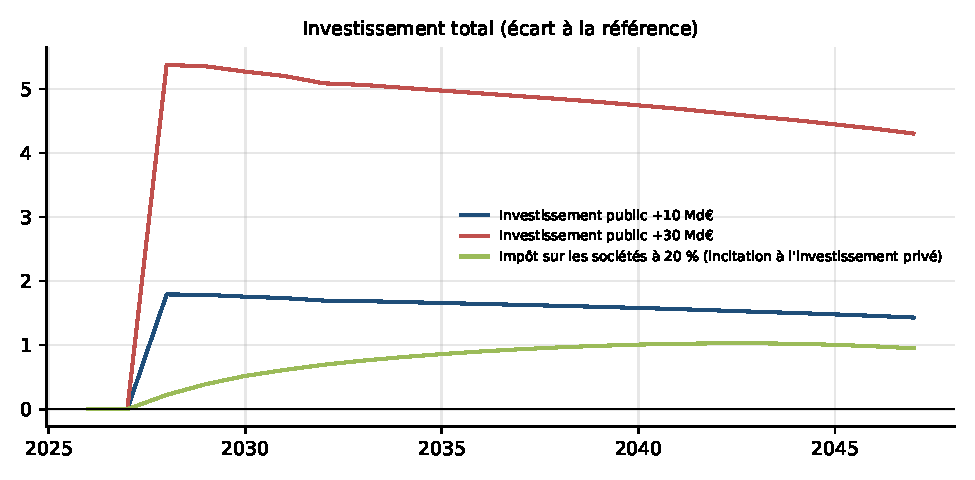
\includegraphics[width=0.85\linewidth]{fbcf_invest.pdf}
\caption{Expérience 5 — Investissement total (écart à la référence).}
\end{figure}

\paragraph{Mécanismes.} L'investissement public agit de deux façons : à court terme comme une demande (avec un
contenu importé élevé, 23~\%), à long terme par l'accumulation d'un capital public qui rend le secteur privé plus
productif (élasticité 0,08). La baisse de l'IS réduit le coût du capital et augmente l'investissement des entreprises
d'environ 1,2~\% à long terme ; une partie des profits libérés est distribuée (50~\%), dont 30~\% à l'étranger.

\paragraph{Résultats.} \textbf{L'investissement public est le seul levier de dépense dont l'effet sur le PIB persiste} :
+10\md{} par an donnent +0,20~\% de PIB en 2029, encore +0,17~\% en 2037 et +0,12~\% en 2047 ; +30\md{} donnent
+0,61~\%, +0,50~\% et +0,35~\%. Il ne s'autofinance pas : 10\md{} dégradent le solde de 0,30 point en 2029 (90~\% de son
coût) et la dette de 10,5 points en 2047. L'emploi augmente à court terme (+24\,000) puis l'effet s'annule : à long terme,
le gain de PIB vient de la productivité, pas de l'emploi. Les importations augmentent de 0,49~\% : un quart de la
dépense « fuit » à l'étranger.

La \textbf{baisse de l'IS} à 20~\% a des effets faibles mais durables : investissement +0,52~\% en 2030, PIB +0,05 à
+0,08~\%, emploi +8\,000 à +18\,000 ; elle coûte 0,56 à 0,63 point de PIB de solde (17 à 19\md) et 19 points de dette en
2047. \fiab{robuste} pour le faible effet, dans le cadre du modèle ; la littérature internationale trouve des effets
plus forts quand on tient compte de la localisation des investissements et des profits.

Les \textbf{logements sociaux} (50\,000 par an, subvention publique de 25~\%) augmentent l'investissement de 1,5~\% et
le PIB de 0,17~\% en 2029 pour un coût budgétaire presque nul ; mais le modèle ne représente ni les loyers, ni la
mobilité, ni le financement par emprunt des bailleurs (\fiab{fragile}).

\paragraph{Investissements productifs et dépenses qui ne le sont pas.} Dans le modèle, la distinction se fait par un seul
paramètre : l'élasticité de la production au capital public (0,08, plage 0,04-0,12 ; 0,12 pour les infrastructures).
Une dépense sans effet d'offre (fonctionnement) a un effet sur le PIB qui disparaît en dix ans ; un investissement public
avec effet d'offre garde un tiers à la moitié de son effet initial au bout de vingt ans. Avec l'élasticité basse (0,04),
l'effet de long terme est divisé par deux ; avec la haute (0,12), il augmente de moitié.

\paragraph{Gagnants et perdants.} Investissement public : entreprises du BTP et de l'équipement, utilisateurs des
infrastructures ; coût porté par la dette. Baisse d'IS : actionnaires (dont 30~\% non résidents), entreprises
capitalistiques.

\paragraph{Conditions d'inversion.} Si l'investissement public est mal choisi (élasticité nulle), il devient une
dépense comme une autre ; si les taux d'intérêt montent fortement en réaction à la dette, l'effet d'éviction réduit le
gain (avec la prime de risque, déjà incluse : +3 points de base par point de dette).

% ====================================================================================================
\section{Expérience 6 : réindustrialiser la France}
\label{sec:exp6}

\paragraph{Situation initiale.} L'industrie manufacturière représente 9,6~\% du PIB en 2025 et continue de reculer dans la
référence. Le contenu en importations est élevé dans la chimie, la pharmacie, la métallurgie, l'électronique, les
équipements électriques, les machines et l'automobile.

\paragraph{Modifications.} Objectif de substitution d'importations : $-$10~\% et $-$20~\% des parts importées de huit produits
industriels, atteint en cinq ans après deux ans de construction des usines, avec un investissement de capacité
(ratio capital / valeur ajoutée de chaque branche) et un surcoût de production de 10~\% par rapport aux importations.
Variantes : avec une énergie importée plus chère de 20~\% ; avec des droits de douane de 10~\% sur les importations hors
Union européenne (et riposte des partenaires) ; droits de douane seuls.

\begin{table}[htbp]
\centering\scriptsize
\caption{Expérience 6 — Réindustrialisation et protection commerciale.}
\label{tab:industrie}
\tabfit{../tableaux/tab_industrie}\\[4pt]
\tabfit{../tableaux/tabd_industrie}
\end{table}

\begin{figure}[htbp]
\centering
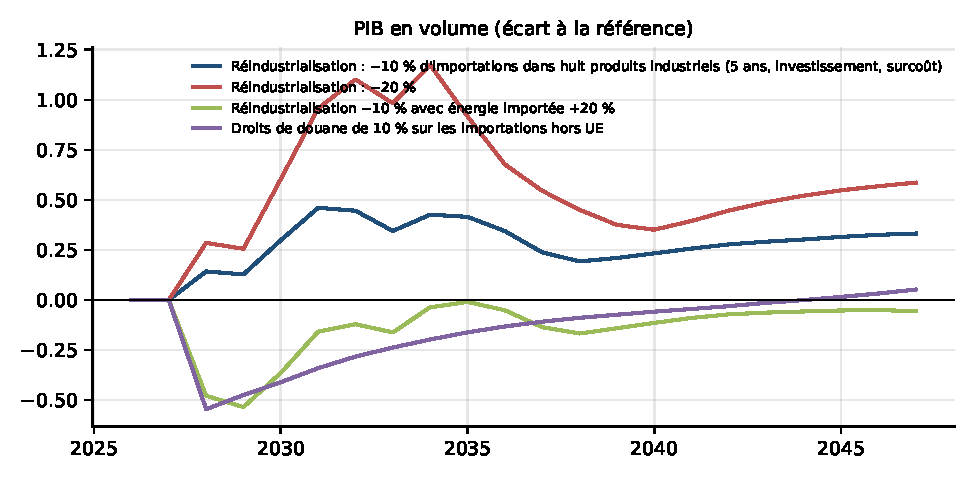
\includegraphics[width=0.95\linewidth]{pib_industrie.pdf}\\
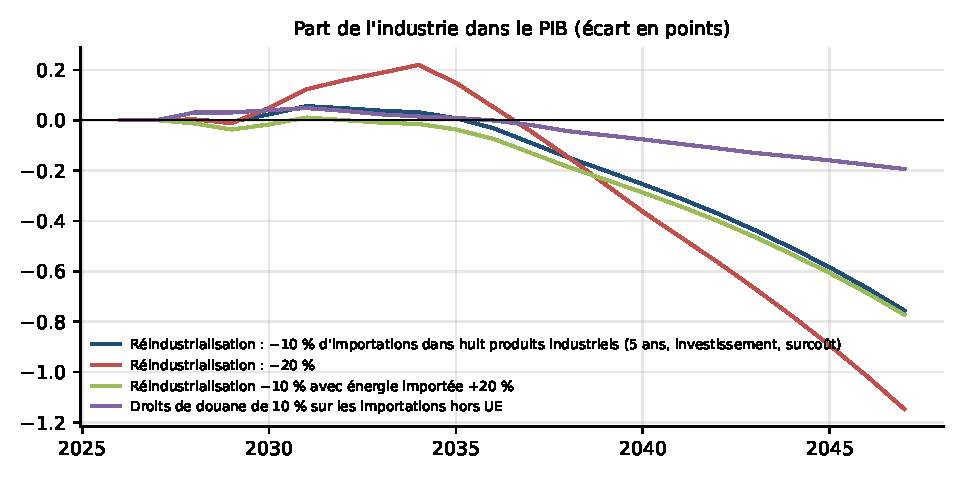
\includegraphics[width=0.95\linewidth]{industrie_part.pdf}
\caption{Expérience 6 — PIB et part de l'industrie dans le PIB.}
\label{fig:industrie}
\end{figure}

\paragraph{Mécanismes.} Produire en France ce qui était importé (1) remplace des importations par de la production
nationale (valeur ajoutée, emplois, revenus, recettes) ; (2) exige d'abord un investissement de capacité (demande
supplémentaire pendant la construction) ; (3) renchérit les produits concernés (surcoût de 10~\%), ce qui se propage aux
prix ; (4) mobilise de la main-d'œuvre, ce qui tend le marché du travail et les salaires.

\paragraph{Résultats.} Une relocalisation de 10~\% augmente le PIB de 0,45~\% en 2032 et l'emploi de 80\,000 ; 20~\%
donne +1,10~\% et +179\,000. L'investissement augmente de 1 à 2~\% pendant la construction. Les prix augmentent de 0,4 à
1,1~\% en 2037 (surcoût). Le solde public s'améliore un peu (+0,17 à +0,37 point en 2032). La part de l'industrie dans le
PIB ne gagne que 0,05 à 0,16 point : \textbf{une relocalisation de 10 à 20~\% des importations de huit produits ne
change pas l'ordre de grandeur du poids de l'industrie}. Après la phase de construction, l'effet sur le PIB diminue
(+0,24~\% en 2037 pour 10~\%) car l'investissement de capacité retombe et le surcoût pèse sur le pouvoir d'achat.

\textbf{Avec une énergie importée plus chère de 20~\%}, la même relocalisation donne un PIB inférieur à la référence
($-$0,54~\% en 2029, $-$0,12~\% en 2032) et une dette plus élevée de 26 points en 2047 : le choc énergétique annule le
gain de la relocalisation. \textbf{Les droits de douane de 10~\%}, avec riposte, réduisent le PIB de 0,47~\% en 2029
(exportations $-$3,3~\%, prix +1,2~\%) ; combinés à la relocalisation, ils en annulent le bénéfice (PIB $-$1,04~\% en
2029, $-$0,45~\% en 2032) : la protection commerciale fait payer aux exportateurs et aux consommateurs ce qu'elle
apporte aux producteurs protégés.

\paragraph{Ce que le modèle ne dit pas.} La relocalisation est ici un \textbf{objectif imposé}, pas le résultat d'une
politique : le modèle ne dit pas comment l'atteindre (aides, compétitivité, énergie, foncier), ni si les qualifications
nécessaires existent (pas de contrainte de main-d'œuvre par métier), ni quelles matières et quels composants seraient
alors importés (dépendances matérielles représentées en valeur seulement). \fiab{fragile} : le résultat est
proportionnel à l'hypothèse de substitution.

\paragraph{Gagnants et perdants.} Gagnants : salariés et territoires industriels, finances publiques ; perdants :
consommateurs des produits relocalisés (surcoût), et, avec des droits de douane, les exportateurs et les ménages
modestes (hausse des prix).

\paragraph{Conditions d'inversion.} Énergie chère, surcoût supérieur à 20~\%, droits de douane avec riposte, ou
relocalisation financée par des aides publiques non chiffrées ici.

% ====================================================================================================
\section{Expérience 7 : modifier les prestations sociales}
\label{sec:exp7}

\paragraph{Modifications.} RSA +25~\% ; prime d'activité +25~\% ; allocations familiales +25~\% ; aides au logement
$-$10~\% ; minimum vieillesse +25~\%.

\begin{table}[htbp]
\centering\scriptsize
\caption{Expérience 7 — Prestations sociales.}
\label{tab:prestations}
\tabfit{../tableaux/tab_prestations}\\[4pt]
\tabfit{../tableaux/tabd_prestations}
\end{table}

\begin{figure}[htbp]
\centering
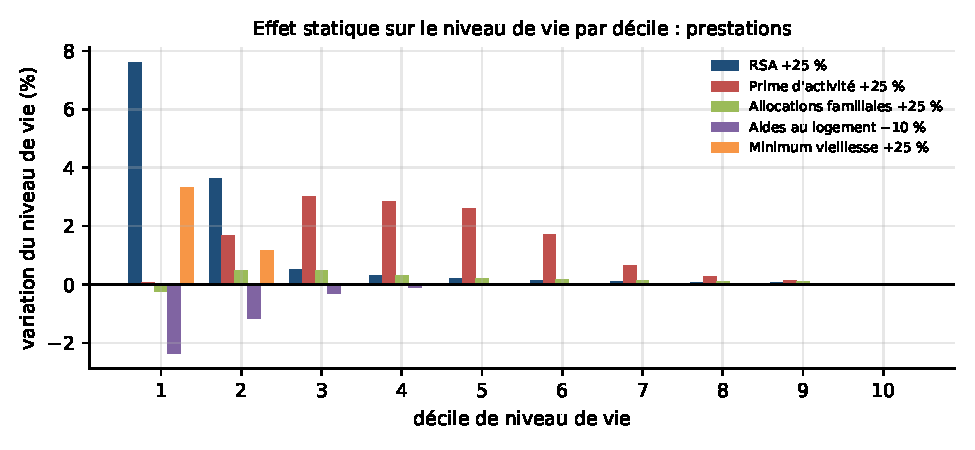
\includegraphics[width=0.9\linewidth]{distribution_prestations.pdf}
\caption{Expérience 7 — Variation statique du niveau de vie par décile.}
\label{fig:distprest}
\end{figure}

\paragraph{Mécanismes.} Une prestation sous condition de ressources augmente le revenu de ménages modestes à forte
propension à consommer $\to$ consommation $\uparrow$ ; elle coûte au budget ; elle modifie les incitations au travail par
le taux marginal effectif (figure~\ref{fig:seuils}).

\paragraph{Résultats.} \textbf{La prime d'activité est le levier le plus efficace contre la pauvreté par euro dépensé
dans le modèle} : +25~\% réduit la pauvreté de 1,43 point (statique) pour un coût de 0,24 point de PIB de solde ; elle
profite aux déciles 2 à 6 (+1,7 à +3~\%). Le RSA +25~\% réduit la pauvreté de 0,33 point et l'indice de Gini de 0,38
point, pour un coût plus faible (0,09 point de PIB) ; il profite au premier décile (+7,6~\%). Les allocations familiales
+25~\% réduisent la pauvreté de 0,55 point ; une partie des ménages du premier décile y perdent (10~\%) parce que les
allocations familiales entrent dans la base ressources du RSA et de la prime d'activité : c'est une interaction entre
barèmes, dont l'ampleur dépend des hypothèses de recours. Le minimum vieillesse +25~\% améliore le niveau de vie des deux
premiers déciles de 3,3 et 1,2~\% pour un coût faible. La baisse des aides au logement de 10~\% augmente la pauvreté de
0,18 point et touche le premier décile ($-$2,4~\%). Effets macroéconomiques : faibles et positifs (PIB +0,03 à +0,25~\%
en 2029), s'estompant à long terme.

\paragraph{Incitations au travail.} Le modèle ne représente pas la réaction de l'offre de travail aux prestations (pas
d'élasticité de participation) : une hausse du RSA, qui augmente le revenu sans emploi, et une hausse de la prime
d'activité, qui augmente le gain à l'emploi, n'ont pas d'effet différent sur l'emploi. Les taux marginaux effectifs de
la figure~\ref{fig:seuils} montrent qu'une hausse de la prime d'activité améliore l'incitation à reprendre un emploi à
temps partiel, mais prolonge la zone de taux marginaux élevés entre 1 et 2 SMIC. \fiab{non établi}.

\paragraph{Conditions d'inversion.} Le non-recours (un tiers des ayants droit au RSA et à la prime d'activité) réduit
l'effet sur la pauvreté ; une réaction négative de l'offre de travail au RSA réduirait son efficacité.

% ====================================================================================================
\section{Expérience 8 : augmenter le temps de travail}
\label{sec:exp8}

\paragraph{Modifications.} Durée légale du travail portée à 37 heures, ou abaissée à 32 heures (mise en place en deux
ans) ; âge légal de départ en retraite porté progressivement à 65 ou 66 ans, ou ramené à 62 ans (trois mois par
génération).

\begin{table}[htbp]
\centering\scriptsize
\caption{Expérience 8 — Durée du travail et âge de départ.}
\label{tab:travail}
\tabfit{../tableaux/tab_travail}\\[4pt]
\tabfit{../tableaux/tabd_travail}
\end{table}

\begin{figure}[htbp]
\centering
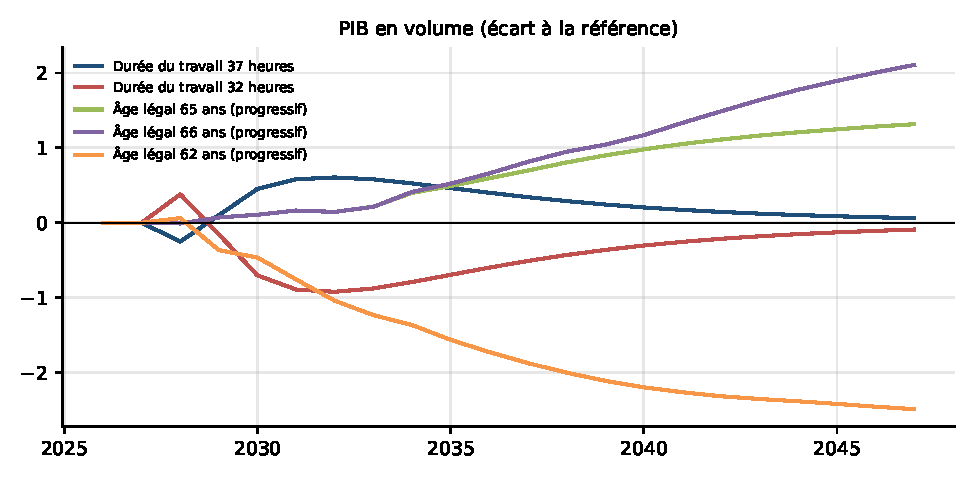
\includegraphics[width=0.95\linewidth]{pib_travail.pdf}\\
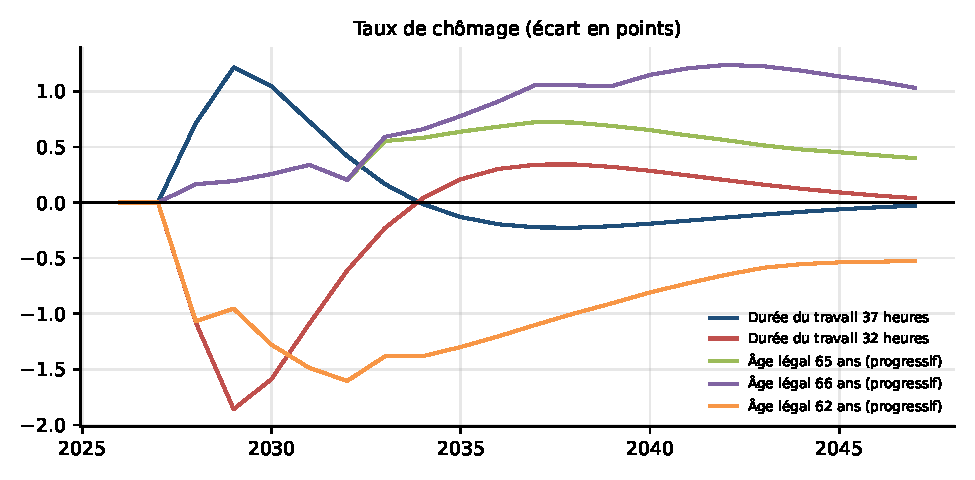
\includegraphics[width=0.95\linewidth]{chomage_travail.pdf}
\caption{Expérience 8 — PIB et chômage.}
\label{fig:travail}
\end{figure}

\paragraph{Mécanismes.} \emph{Durée hebdomadaire} : le modèle suppose que 70~\% d'une variation des heures est absorbée
sans changement d'effectif (productivité horaire, intensité, heures supplémentaires) et que les salaires mensuels sont
maintenus \preuve{H, calé sur l'ordre de grandeur des 35 heures}. Allonger la durée augmente donc la production par
salarié : les entreprises ont besoin de moins de salariés pour la même production, le coût horaire baisse. \emph{Âge de
départ} : plus d'actifs (offre de travail), moins de pensions ; les seniors maintenus actifs sont en emploi à 89~\%
la première année, mais l'économie doit créer les emplois correspondants (fermeture d'offre).

\paragraph{Résultats.} \textbf{37 heures} : la production par tête augmente, mais \textbf{l'emploi baisse fortement à
court terme} ($-$408\,000 en 2029, chômage +1,05 point) parce que la demande ne suit pas immédiatement l'offre ; la baisse
du coût horaire réduit les prix ($-$1,25~\%) et soutient les exportations (+0,9~\%) ; le PIB augmente (+0,60~\% en 2032)
à mesure que la fermeture d'offre résorbe le chômage ; en 2037, l'emploi redevient supérieur à la référence (+76\,000).
\textbf{32 heures} : effet inverse, emploi +624\,000 en 2029 (partage du travail), chômage $-$1,6 point, mais PIB
$-$0,92~\% en 2032, prix +2~\% et exportations $-$1,3~\% ; à long terme, l'emploi devient inférieur à la référence.

\textbf{Âge de départ à 65 ans} : le PIB augmente lentement (+0,14~\% en 2032, +0,70~\% en 2037, +1,31~\% en 2047) avec la
population active ; le chômage augmente d'abord (+0,26 point en 2030), le temps que l'emploi rattrape ; 66 ans : +2,1~\%
de PIB en 2047. \textbf{Retour à 62 ans} : PIB $-$1,04~\% en 2032, $-$2,5~\% en 2047 ; emploi $-$570\,000 en 2037 ; le chômage
baisse (moins d'actifs) ; les pensions augmentent.

Un résultat contre-intuitif mérite d'être signalé : \textbf{le report de l'âge à 65 ans n'améliore presque pas le
ratio de dette dans le modèle} (+0,9 point en 2047 alors que le solde s'améliore de 0,16 à 0,18 point). L'afflux
d'actifs augmente d'abord le chômage, ce qui modère les salaires et les prix ($-$0,9~\% en 2037) : le PIB nominal, au
dénominateur du ratio, est plus bas. Ce mécanisme de prix est \fiab{fragile} (courbe de Phillips calibrée) ; l'effet sur
les pensions (moins de pensions versées) est \fiab{robuste}.

\paragraph{Gagnants et perdants.} 37 heures : salariés en emploi (même salaire, plus d'heures : baisse du salaire
horaire), entreprises ; perdants : chômeurs supplémentaires à court terme. Report de l'âge : finances sociales et
actifs futurs ; perdants : générations concernées (carrières plus longues, en particulier les métiers pénibles, non
distingués dans le modèle).

\paragraph{Conditions d'inversion.} Si l'économie absorbe les actifs supplémentaires plus vite (fermeture forte), le
gain de PIB du report de l'âge arrive plus tôt ; si elle ne les absorbe pas (fermeture nulle), le report augmente
durablement le chômage. La contre-expertise donne, pour un retour à 62 ans, une plage de $-$2,4~\% à +0,3~\% de PIB en
2032 : \fiab{fragile}. Pour la durée hebdomadaire, tout dépend de l'hypothèse de compensation (70~\%), qui n'est pas
estimée : \fiab{fragile}.

\begin{resultat}
Travailler plus (durée ou carrière) augmente la production à long terme, mais pas immédiatement : à court terme,
l'économie doit créer les emplois correspondants, et le chômage augmente d'abord. Réduire le temps de travail partage
l'emploi existant à court terme mais réduit la production et la compétitivité.
\end{resultat}

\chapter{Mécanismes complémentaires et interactions}
\label{ch:complementaires}

\section{Prix de l'énergie, désindustrialisation et pouvoir d'achat}

\paragraph{Expérience.} Prix de l'énergie importée (produits extractifs, raffinage, électricité-gaz) +50~\% à partir de
2028, ou $-$20~\%. Ce n'est pas une mesure mais un choc d'environnement.

\begin{table}[htbp]
\centering\scriptsize
\caption{Chocs d'environnement et mesures complémentaires.}
\label{tab:complementaires}
\tabfit{../tableaux/tab_complementaires}\\[4pt]
\tabfit{../tableaux/tabd_complementaires}
\end{table}

\paragraph{Mécanismes et résultats.} La hausse se transmet aux prix à la consommation (la moitié la première année) et aux
coûts de toutes les branches selon leur contenu direct et indirect en énergie. Les prix augmentent de 4,4~\% en 2030 ;
le pouvoir d'achat recule de 3,2~\% ; la consommation de 2,8~\% ; les exportations de 2,8~\% (perte de compétitivité) ;
l'emploi de 225\,000 en 2029 et 328\,000 en 2032 ; le PIB de 1,2~\% en 2029. Le solde public se dégrade de 0,7 point en
2029 puis de 1,4 point en 2032, et la dette s'alourdit de 15 points en 2037 et 49 points en 2047. Le solde extérieur
perd 2,3 points de PIB. La part de l'industrie dans le PIB ne varie presque pas ($-$0,02 point) : \textbf{le modèle ne
représente pas la désindustrialisation par le prix de l'énergie} (pas de fermeture de sites, pas de substitution, pas
de relocalisation de la production énergivore à l'étranger) ; l'effet sur l'industrie est donc \fiab{non établi}, et
probablement sous-estimé pour les branches énergivores (chimie, métallurgie). Une baisse de 20~\% a des effets
symétriques et proportionnels.

\paragraph{Importations et pouvoir d'achat.} Ce choc illustre la relation entre importations et pouvoir d'achat : la
France ne produit ni pétrole ni gaz ; un renchérissement de ces importations est un transfert de revenu vers le reste du
monde, que ni les salaires (indexés en partie et avec retard) ni le budget ne peuvent compenser sans coût. La
comparaison avec l'expérience des droits de douane (chapitre précédent) est instructive : une hausse du prix des
importations, qu'elle vienne des marchés ou de droits de douane, réduit le pouvoir d'achat ; la différence est que la
recette des droits de douane reste en France (en partie), alors que le surcoût énergétique part à l'étranger.

\section{Inflation et dette publique}

Une inflation plus élevée réduit-elle le poids de la dette ? Le modèle permet de distinguer trois canaux, que les
expériences précédentes mettent en évidence :
\begin{enumerate}
\item \textbf{l'effet de dénominateur} : la dette est fixée en euros ; le PIB nominal augmente avec les prix. Une hausse
générale des salaires de 2~\% (+1,3~\% de prix) réduit le ratio de dette de 3 points en 2032 ;
\item \textbf{l'effet de décalage d'indexation} : les recettes suivent les prix immédiatement, les prestations avec un an
de retard, les rémunérations publiques selon les décisions ; une inflation qui surprend améliore temporairement le
solde ;
\item \textbf{l'effet de taux} : si l'inflation provient d'un choc commun à la zone euro, la BCE relève ses taux (règle
de M11 : 0,39 point de taux par point d'inflation à court terme, 1,44 à long terme) et le taux apparent de la dette
monte progressivement (un huitième par an).
\end{enumerate}
Le test « inflation importée persistante » (+2~\% par an de 2028 à 2032 sur les prix d'importation et des concurrents)
montre que ces effets se compensent presque : la dette de référence en 2037 passe de 178,8 à 178,3~\% du PIB. Une
inflation importée n'allège pas la dette : elle appauvrit le pays et relève les taux. Seule une inflation \emph{intérieure}
non anticipée (hausse des salaires et des prix) réduit le ratio, au prix d'un transfert des créanciers et des
titulaires de revenus fixes vers l'État. \fiab{fragile} : dépend de la courbe de Phillips et de la règle de taux.

\section{Fiscalité, croissance et redistribution}

Les expériences 1 et 7 permettent de mesurer l'arbitrage entre redistribution et activité. Les mesures redistributives
vers le bas de la distribution (RSA, prime d'activité, minimum vieillesse) \emph{soutiennent} l'activité à court terme
dans le modèle, parce que les ménages modestes consomment davantage ; les hausses d'impôts sur le haut de la
distribution (ISF, PFU, tranche supérieure de l'IR) la réduisent peu. L'expérience combinée « RSA et prime d'activité
+25~\%, financés par +0,5 point de CSG » le confirme : PIB +0,27~\% en 2029, emploi +60\,000, pauvreté $-$1,65 point,
indice de Gini $-$0,95 point, mais solde $-$0,20 point (la CSG à +0,5 point ne finance qu'environ la moitié de la
dépense). Les gagnants sont les six premiers déciles (+7,5~\% pour le premier, +2,4~\% pour le cinquième) ; les perdants,
les quatre derniers ($-$0,1 à $-$0,4~\%).

\textbf{Ce résultat dépend d'une hypothèse} : le modèle ignore les effets des prélèvements et des prestations sur
l'offre de travail, l'épargne et l'investissement à long terme (participation, heures, effort, entrepreneuriat,
accumulation de patrimoine). La littérature économique trouve ces effets modestes pour les ménages modestes et plus
importants pour les hauts revenus et les revenus du capital (élasticités de M13). Le modèle n'est donc pas en mesure
de trancher le débat sur l'arbitrage de long terme entre équité et efficacité \fiab{non établi} ; il montre seulement
qu'à court et moyen terme, la redistribution vers les ménages modestes n'est pas coûteuse en activité.

\section{Salaires et compétitivité}

L'expérience 2 montre que, dans le modèle, une hausse générale des salaires de 2~\% réduit les exportations de 0,6~\%
et que la baisse de 20\md{} des cotisations (expérience 4) les augmente de 0,4~\%. La compétitivité-prix est donc un
canal réel mais d'ampleur limitée : l'élasticité-prix des exportations est de $-$0,6, celle des importations de $-$0,11
seulement (inférieure à la littérature). Le modèle sous-estime probablement la perte de parts de marché intérieures
après une hausse des coûts, et il ne représente ni la compétitivité hors prix (qualité, innovation), ni la distinction
entre secteurs exposés et abrités \fiab{fragile}.

\section{Automatisation et emploi}

Le modèle ne contient pas de mécanisme d'automatisation au sens d'un progrès technique qui remplacerait certaines tâches.
Deux paramètres en tiennent lieu : la tendance de productivité de chaque branche (exogène) et l'élasticité de
substitution capital-travail $\sigma$, qui détermine combien d'emplois sont remplacés par du capital quand le coût du
travail augmente. La contre-expertise donne, pour une hausse de coût du travail, une variation de l'emploi d'environ
$\pm$25\,000 selon que $\sigma$ vaut 0,2 ou 0,7. Un choc d'automatisation (productivité plus forte de 0,3 point par
an) se traduirait dans le modèle par \emph{moins d'emplois pour la même production}, sans hausse du PIB, parce que la
production y est déterminée par la demande à moyen terme : c'est une limite importante, qui conduit aussi à un résultat
paradoxal pour le test de robustesse « productivité plus faible » (section~\ref{sec:paradoxe}).

\section{Endettement, taux d'intérêt et investissement}

La dette publique réagit fortement aux taux : une hausse durable de 1,5 point des taux longs porte la dette de
référence de 179 à 191~\% du PIB en 2037 et de 308 à 359~\% en 2047. Par la prime de risque (3 points de base par point
de dette), un programme qui augmente la dette de 10 points relève les taux de 0,3 point. Le coût d'usage du capital
augmente avec les taux et réduit l'investissement des entreprises (élasticité $-$0,18) : l'expérience de l'investissement
public financé par la dette (+30\md) montre un effet d'éviction faible dans le modèle (prime de risque modeste, BCE qui
ne réagit qu'à l'activité de toute la zone). \fiab{fragile} : la prime de risque est une hypothèse, et le modèle ne
représente pas de crise de financement (pas de non-linéarité, pas de perte de confiance).

\section{Dépenses publiques et croissance potentielle}

Dans le modèle, seul l'investissement public élève durablement la production (élasticité 0,08). Les autres dépenses ont
un effet de demande qui disparaît en une dizaine d'années. C'est une hypothèse conservatrice : l'éducation, la
recherche, la santé et la formation ont, selon une littérature abondante, des effets de long terme sur la productivité
et la participation, mais leur ampleur est incertaine et dépend de la qualité des dépenses. Le modèle ne peut donc pas
classer les dépenses publiques selon leur efficacité de long terme. \fiab{non établi}.

\section{Démographie et soutenabilité du système social}
\label{sec:paradoxe}

La référence montre la pression démographique : le rapport entre les 65 ans ou plus et les 20-64 ans passe de 0,39 à
0,51 de 2025 à 2047 ; les pensions de 13,5 à 15,7~\% du PIB. Les leviers démographiques internes au système
(âge de départ, indexation) sont analysés à l'expérience 8 et au chapitre~\ref{ch:experiences} : le report de l'âge
légal à 65 ans réduit les pensions et augmente la production à long terme (+1,3~\% en 2047) ; une sous-indexation d'un
point par an réduit les pensions de 0,56 point de PIB dès 2032.

\begin{limites}[Un paradoxe révélateur : les chocs d'offre]
Deux tests de robustesse du chapitre~\ref{ch:strategie} appliquent des chocs d'offre à la référence : une productivité plus
faible de 0,3 point par an et une population active plus faible de 0,2~\% par an. Dans les deux cas, le modèle donne
\emph{moins de chômage} (6,6~\% au lieu de 7~\% en 2037 pour la productivité ; 6,1~\% pour la démographie) et une dette
légèrement \emph{plus basse} (174 et 177~\% du PIB au lieu de 179 en 2037). Ce résultat contredit l'intuition et la
plupart des modèles d'offre : moins de travailleurs ou des travailleurs moins productifs devraient réduire la production
potentielle, donc les recettes. Il s'explique par la structure du modèle : à moyen terme, la production y est
déterminée par la demande ; un choc d'offre négatif réduit le chômage (moins d'actifs ou plus d'emplois nécessaires pour
la même production), ce qui accélère les salaires et les prix et gonfle le PIB nominal. La fermeture d'offre ne ramène
le chômage vers son niveau structurel que lentement. \textbf{Les effets des chocs de productivité et de démographie sur
le PIB et la dette ne sont donc pas fiables dans cette version} \fiab{non établi} ; ils signalent la priorité
d'amélioration n\textsuperscript{o}1 de la contre-expertise (estimer la fermeture d'offre et relier explicitement
la production potentielle au travail et à la productivité).
\end{limites}

\section{Effets cumulés : pourquoi une mesure ne s'évalue pas seule}
\label{sec:interactions}

Cinq combinaisons ont été simulées et comparées à la somme des effets des mesures isolées (figure~\ref{fig:interactions}).

\begin{figure}[htbp]
\centering
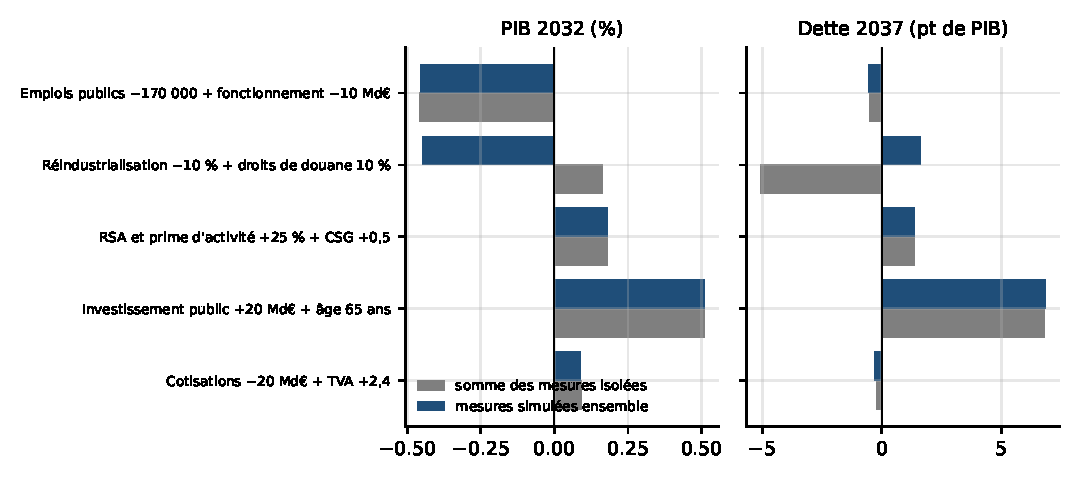
\includegraphics[width=\linewidth]{interactions.pdf}
\caption{Mesures combinées : somme des effets isolés (gris) et simulation conjointe (bleu).}
\label{fig:interactions}
\end{figure}

\begin{table}[htbp]
\centering\scriptsize
\caption{Mesures combinées et mesures isolées.}
\label{tab:interactions}
\tabfit{../tableaux/tab_interactions}
\end{table}

\begin{enumerate}
\item \textbf{Mesures qui se neutralisent : relocalisation et droits de douane.} Isolée, la relocalisation de 10~\%
augmente le PIB de 0,45~\% en 2032 ; les droits de douane avec riposte le réduisent de 0,28~\%. Simulées ensemble, elles
le réduisent de 0,45~\%, soit 0,6 point de moins que la somme ; la dette est plus élevée de 1,6 point en 2037 au lieu
d'être plus basse de 5 points. Les deux mesures se nuisent : la riposte frappe les exportations de l'industrie que la
relocalisation veut développer, et la hausse des prix importés renchérit ses consommations intermédiaires. \emph{Une
politique industrielle combinée à une protection commerciale peut détruire ce qu'elle cherche à créer.}
\item \textbf{Mesures qui se compensent : TVA sociale.} La baisse de cotisations augmente l'emploi et baisse les prix ; la
hausse de TVA fait l'inverse. Ensemble, les effets sont presque additifs : PIB +0,09~\% en 2032, solde neutre. Le
transfert de charge vers la consommation fait des perdants (retraités, ménages modestes) qui ne sont pas les gagnants.
\item \textbf{Mesures qui se renforcent : investissement public et âge de départ.} L'investissement public augmente la
demande quand le report de l'âge augmente l'offre de travail : les actifs supplémentaires trouvent plus vite un emploi.
L'effet combiné sur le PIB (+0,51~\% en 2032, +1,03~\% en 2037) est proche de la somme ; le chômage est moins élevé
qu'avec le report seul.
\item \textbf{Mesures qui s'additionnent : prestations financées par la CSG} (section précédente) et \textbf{économies
d'emploi public et de fonctionnement} ($-$0,45~\% de PIB en 2032, $-$145\,000 emplois) : effets additifs.
\end{enumerate}

\begin{resultat}
Les mesures budgétaires et redistributives s'additionnent presque exactement dans le modèle ; les mesures qui touchent
les prix, le commerce extérieur et l'offre de travail interagissent fortement. C'est pourquoi les programmes de la
partie~III, construits à partir de mesures isolées, ont tous été re-simulés avec le modèle complet.
\end{resultat}


\part{Construire une stratégie de redressement}
\chapter{Stratégies de redressement : recherche, comparaison, robustesse}
\label{ch:strategie}

\section{Point de départ : des objectifs qui ne sont pas tous compatibles}

La mission fixe douze objectifs simultanés : moins de chômage, plus de niveau de vie médian, moins de pauvreté, plus de
pouvoir d'achat, de productivité, de croissance et de compétitivité, moins de déficit et de dette, une meilleure balance
commerciale, plus de souveraineté industrielle et énergétique, une protection sociale soutenable. Les expériences des
chapitres précédents montrent que ces objectifs entrent en tension :

\begin{itemize}
\item \textbf{déficit contre activité à court terme} : toute consolidation budgétaire réduit l'activité la première année
(de 0,3 à 2,1~\% de PIB par point de solde gagné selon l'instrument) ;
\item \textbf{déficit contre pouvoir d'achat} : les instruments les moins coûteux en activité (TVA, taxe carbone,
désindexation) réduisent le pouvoir d'achat de tous les ménages et pèsent davantage sur les modestes ;
\item \textbf{pauvreté contre déficit} : les prestations ciblées réduisent efficacement la pauvreté mais coûtent ;
\item \textbf{production à long terme contre chômage à court terme} : allonger la durée du travail ou les carrières
augmente la production à long terme mais d'abord le chômage ;
\item \textbf{souveraineté industrielle contre pouvoir d'achat} : relocaliser renchérit les produits ; protéger par des
droits de douane fait payer les consommateurs et les exportateurs ;
\item \textbf{dette contre investissement} : l'investissement public est le seul levier de dépense qui accroît durablement
la production, mais il ne s'autofinance pas.
\end{itemize}

Le modèle ne peut pas arbitrer entre ces objectifs : c'est un choix de société. Il peut en revanche chercher, pour une
pondération explicite des objectifs, les combinaisons de mesures qui donnent le meilleur résultat, et vérifier leur
cohérence. C'est ce que fait ce chapitre.

\section{Méthode : un méta-modèle linéaire et une optimisation sous contraintes}

\paragraph{Étape 1 : méta-modèle.} Chaque levier est représenté par la pente de ses effets, mesurée sur les expériences
des chapitres~\ref{ch:experiences} et~\ref{ch:complementaires} : effet par unité de curseur sur chaque indicateur (PIB,
emploi, chômage, solde, dette, solde extérieur, revenu national, industrie, pouvoir d'achat, pauvreté, médiane, inflation)
et chaque horizon (2029, 2030, 2032, 2037, 2047). Les hausses et les baisses d'un même levier ont des pentes distinctes.
L'effet d'un programme est approché par la somme des effets de ses mesures.

\paragraph{Étape 2 : programmes linéaires.} Pour chaque scénario, on maximise une fonction objectif linéaire sous
contraintes linéaires (méthode HiGHS, bibliothèque scipy), pour chacune des quatre règles d'âge de départ (64 ans,
actuelle ; 62, 65 et 66 ans) ; la meilleure est retenue. Une \textbf{pénalité de parcimonie} (coût fixe par levier
utilisé à pleine amplitude) évite les programmes qui actionnent tous les leviers d'un epsilon.

\paragraph{Contraintes de faisabilité communes} (hypothèses explicites, identiques pour tous les scénarios) :
\begin{itemize}
\item amplitude de chaque levier limitée à la plage testée par les expériences (pas d'extrapolation au-delà) ;
\item hausses de prélèvements limitées à 1,5 point de PIB et économies de dépenses à 2,5 points de PIB (effet sur le
solde en 2030), sur un mandat ;
\item \textbf{leviers exclus} : hausse de l'IS et des impôts de production (leur coût passe par la délocalisation des
bénéfices et des activités, que le modèle ne représente pas : il en sous-estimerait le coût) ; réindustrialisation
(c'est un objectif, pas un instrument : le modèle n'en représente pas le coût public) ; SMIC (l'emploi peu qualifié n'est
pas représenté).
\end{itemize}

\paragraph{Étape 3 : vérification.} Chaque programme est re-simulé avec le modèle complet (microsimulation comprise),
puis soumis à sept chocs d'environnement et à une mise en œuvre partielle.

\begin{table}[htbp]
\centering\small
\caption{Fonctions objectifs et contraintes des scénarios (écarts à la référence).}
\label{tab:objectifs}
\begin{tabularx}{\linewidth}{@{}p{2.4cm}LL@{}}
\toprule
Scénario & Objectif maximisé & Contraintes \\
\midrule
A — budgétaire & Réduire la dette en 2037 & PIB 2030 $\geq -0{,}5$~\% ; chômage 2030 $\leq$ +0,3 pt ; pauvreté 2037 $\leq 0$ ; pouvoir d'achat 2030 $\geq -1$~\% \\
B — croissance & PIB 2037 + part de l'industrie 2037 & dette 2037 $\leq 0$ ; solde 2030 $\geq 0$ ; pauvreté $\leq$ +0,2 pt \\
C — équilibré & PIB 2037 + emploi 2037 / 200\,000 $-$ 2 $\times$ pauvreté + pouvoir d'achat 2037 & dette 2037 $\leq -5$ pt ; solde 2030 $\geq$ +0,5 pt ; pauvreté $\leq 0$ ; chômage 2030 $\leq$ +0,2 pt \\
D — effort maximal & Réduire la dette en 2047 & plafonds relevés à 2,5 pt (impôts) et 4 pt (dépenses) ; PIB 2030 $\geq -1{,}5$~\% ; pauvreté $\leq 0$ \\
\bottomrule
\end{tabularx}
\end{table}

\begin{encadre}{Encadré 7.1 — Ce qu'une optimisation peut et ne peut pas dire}
Un programme « optimal » au sens mathématique est la meilleure combinaison \emph{pour la fonction objectif choisie, dans
le modèle, avec ses hypothèses}. Changer la pondération des objectifs change la solution ; changer une hypothèse du modèle
(fermeture d'offre, élasticités) aussi. L'optimiseur a en outre tendance à exploiter les angles morts du modèle : lors des
premiers essais, il choisissait massivement les hausses d'IS et d'impôts de production, dont le modèle ne voit pas le
coût, ou retenait le retour à 62 ans pour réduire le chômage (moins d'actifs), ce qui n'a pas de sens économique. Ces
solutions ont été écartées par les exclusions et contraintes décrites plus haut. \textbf{Aucune des solutions ci-dessous
n'est un optimum politique ou social.}
\end{encadre}

\section{Les quatre programmes}

\begin{table}[htbp]
\centering\small
\caption{Leviers retenus par l'optimisation (valeur du curseur ; « -- » : inchangé). La colonne R, programme recommandé, est présentée au
chapitre~\ref{ch:synthese}.}
\label{tab:scmesures}
\tabfit{../tableaux/scenarios_mesures}
\end{table}

\paragraph{Scénario A — redressement budgétaire prioritaire.} L'optimiseur combine des hausses d'impôts sur la
consommation (TVA +2 points au taux normal et aux taux réduits, taxe carbone +23~€/t), les droits de succession (+50~\%),
une hausse des cotisations employeurs (+10\md) et une baisse de l'investissement public ($-$10\md), et utilise une partie
de la marge pour la prime d'activité (+25~\%) — qui neutralise l'effet des taxes sur la pauvreté — et un peu de
dépense de fonctionnement (+2,4\md) qui limite la perte d'activité. Âge de départ inchangé.

\paragraph{Scénario B — croissance et réindustrialisation prioritaires.} Le report de l'âge à 66 ans, l'investissement
public (+30\md) et le passage aux 37 heures sont les moteurs de la croissance ; ils sont financés par la TVA, les droits
de succession, les cotisations, la baisse des allocations chômage ($-$25~\%). La réindustrialisation n'étant pas un
instrument, l'objectif « industrie » est peu sensible aux leviers disponibles.

\paragraph{Scénario C — redressement équilibré.} Il combine une forte redistribution vers les ménages modestes (RSA,
prime d'activité, allocations familiales et minimum vieillesse +25~\%, baisse de la TVA de 0,9 point et de la CSG d'un
point), financée par les impôts sur le patrimoine et le capital (ISF à 1~\%, PFU +15 points, successions +50~\%), les
cotisations employeurs et la baisse des allocations chômage ; le report de l'âge à 66 ans soutient la production à long
terme. 50\,000 emplois publics sont créés, l'investissement public baisse de 10\md.

\paragraph{Scénario D — effort maximal sur la dette.} Avec des plafonds relevés, l'optimiseur mobilise presque tous les
leviers de recettes et d'économies : TVA, CSG, IR, ISF, PFU, successions, taxe carbone (+54~€/t), cotisations, fonctionnement
($-$13,6\md), investissement public, sous-indexation des pensions, allocations chômage, durée du travail (37 heures),
droits de douane ; il préserve la pauvreté par la prime d'activité et les allocations familiales.

\section{Vérification avec le modèle complet}

Le méta-modèle additif reproduit le modèle complet à quelques centièmes près pour A et C, et à quelques dixièmes près pour
B et D, qui combinent des chocs d'offre et de prix :
\begin{center}\small
\begin{tabular}{@{}lrrrrrrrr@{}}
\toprule
 & \multicolumn{2}{c}{PIB 2030 (\%)} & \multicolumn{2}{c}{PIB 2037 (\%)} & \multicolumn{2}{c}{Dette 2037 (pt)} & \multicolumn{2}{c}{Dette 2047 (pt)} \\
 & méta & complet & méta & complet & méta & complet & méta & complet \\
\midrule
A & $-$0,43 & $-$0,43 & $-$0,19 & $-$0,19 & $-$14,9 & $-$14,9 & $-$44,7 & $-$43,5 \\
B & +0,93 & +0,88 & +1,79 & +1,77 & 0,0 & $-$0,3 & $-$0,8 & $-$2,7 \\
C & +0,36 & +0,36 & +1,00 & +1,00 & $-$5,7 & $-$5,7 & $-$14,0 & $-$14,3 \\
D & $-$1,50 & $-$1,46 & $-$0,24 & $-$0,23 & $-$28,0 & $-$28,1 & $-$95,9 & $-$89,9 \\
\bottomrule
\end{tabular}
\end{center}

\section{Résultats aux quatre horizons}

\begin{figure}[htbp]
\centering
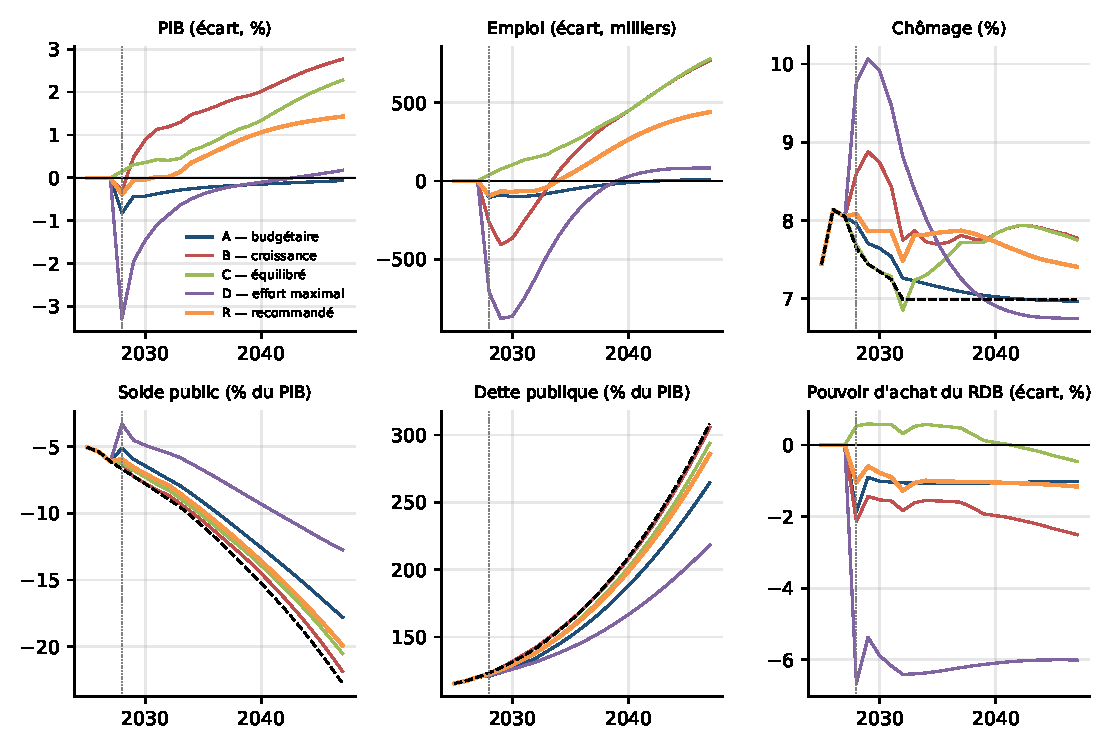
\includegraphics[width=\linewidth]{scenarios.pdf}
\caption{Trajectoires des scénarios (modèle complet). Les panneaux du chômage, du solde et de la dette donnent les niveaux,
avec la référence en tirets ; les autres, les écarts à la référence. Les mesures commencent en 2028.}
\label{fig:scenarios}
\end{figure}

\begin{table}[p]
\centering\scriptsize
\caption{Scénario A — redressement budgétaire prioritaire (modèle complet).}\label{tab:scA}
\tabfit{../tableaux/scenario_A}\\[10pt]
\caption{Scénario B — croissance et réindustrialisation prioritaires.}\label{tab:scB}
\tabfit{../tableaux/scenario_B}
\end{table}

\begin{table}[p]
\centering\scriptsize
\caption{Scénario C — redressement équilibré.}\label{tab:scC}
\tabfit{../tableaux/scenario_C}\\[10pt]
\caption{Scénario D — effort maximal sur la dette.}\label{tab:scD}
\tabfit{../tableaux/scenario_D}
\end{table}

\paragraph{Scénario A.} \emph{Court terme (2029-2030)} : le solde s'améliore de 1,3 point de PIB, au prix d'un PIB plus
bas de 0,43~\%, de 88\,000 à 101\,000 emplois en moins (chômage +0,3 point) et d'un pouvoir d'achat réduit d'un point ;
les prix sont plus élevés de 2,4~\% (TVA, taxe carbone). \emph{Moyen et long terme} : la perte d'activité s'estompe
($-$0,19~\% en 2037), l'amélioration du solde s'accumule (+2,1 points en 2037, +5 en 2047 grâce aux intérêts
économisés), la dette est plus basse de 15 points en 2037 et de 44 points en 2047. \emph{Distribution} : la pauvreté
baisse légèrement ($-$0,24 point) grâce à la prime d'activité, mais le premier décile perd 3,2~\% de niveau de vie (ménages
sans revenu d'activité, qui subissent la TVA sans bénéficier de la prime d'activité) et les déciles 6 à 10 perdent 1 à
2,3~\%. \textbf{Le coût porte sur le pouvoir d'achat, de façon durable} ($-$1~\% jusqu'en 2047).

\paragraph{Scénario B.} \emph{Court terme} : le PIB augmente (+0,5 à +0,9~\%) grâce à l'investissement public, mais
\textbf{le passage aux 37 heures détruit d'abord 409\,000 emplois} (chômage 8,9~\% en 2029 au lieu de 7,4~\%) : la
production par salarié augmente plus vite que la demande. \emph{Moyen terme} : le chômage reflue (7,8~\% en 2032) et le PIB
progresse (+1,2~\% en 2032, +1,8~\% en 2037, +2,8~\% en 2047) ; l'emploi devient supérieur à la référence à partir de
2035 environ (+293\,000 en 2037). \emph{Finances publiques} : neutres par construction (contrainte dette 2037 $\leq 0$).
\emph{Pouvoir d'achat} : $-$1,4 à $-$2,5~\%, car le salaire horaire baisse (37 heures payées 35) et les prix diminuent moins
que les revenus des ménages. Le chômage reste plus élevé que dans la référence de 0,8 point jusqu'en 2047, parce que la
population active augmente continûment avec le report progressif à 66 ans : l'économie absorbe les actifs supplémentaires
avec retard. Pauvreté +0,38 point (statique). \textbf{Le scénario B achète de la production future avec du chômage et
du pouvoir d'achat présents.}

\paragraph{Scénario C.} \emph{Court terme} : PIB +0,3~\%, emploi +75\,000 à +104\,000, chômage stable, pouvoir d'achat
+0,6~\%, solde +0,5 point. \emph{Long terme} : PIB +1,0~\% en 2037 et +2,3~\% en 2047 (report de l'âge), dette $-$5,7 points
en 2037 et $-$14 points en 2047. \emph{Distribution} : c'est le scénario le plus redistributif : pauvreté $-$2,9 points,
indice de Gini $-$1,7 point, niveau de vie médian +4,2~\% (statique) ; le premier décile gagne 11,7~\%, le dernier perd
1,1~\%. \emph{Points faibles} : la consolidation est modeste (+0,5 à +0,9 point de solde) ; à partir de 2035, le chômage
dépasse celui de la référence (+0,7 point) pour la même raison que dans B (report de l'âge) ; la baisse des allocations
chômage repose sur une hypothèse non estimée.

\paragraph{Scénario D.} \emph{Court terme} : récession marquée, PIB $-$2,0~\% en 2029, 879\,000 emplois en moins
(chômage 10,1~\%), pouvoir d'achat $-$5,4~\%. \emph{Long terme} : le PIB revient à la référence vers 2040 ; le solde
s'améliore de 2,7 points dès 2029 et de 4,9 points en 2037 ; la dette est plus basse de 28 points en 2037 (151~\% au lieu
de 179~\%) et de 90 points en 2047. Le pouvoir d'achat reste inférieur de 6~\% à la référence. Tous les déciles perdent
(de 1,3 à 6,8~\%). \textbf{Le scénario D montre ce que coûte, dans le modèle, une stabilisation rapide de la dette :
une récession de deux ans et une baisse durable du pouvoir d'achat.}

\begin{figure}[htbp]
\centering
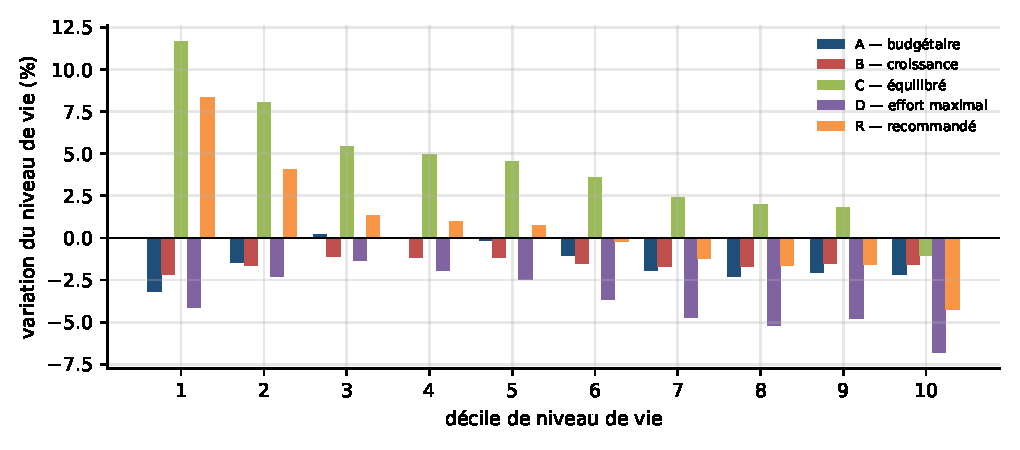
\includegraphics[width=0.95\linewidth]{scenarios_distribution.pdf}
\caption{Variation statique du niveau de vie par décile dans chaque scénario (microsimulation ; mesures fiscales et
sociales seulement, hors effets macroéconomiques).}
\label{fig:scdist}
\end{figure}

\begin{resultat}[Le constat central : aucun scénario ne stabilise la dette]
Dans les cinq scénarios, la dette publique continue d'augmenter en part du PIB jusqu'en 2047 (de 151~\% à 179~\% du PIB en
2037, de 218~\% à 306~\% en 2047). La référence suppose un taux d'intérêt de 4,89~\% maintenu vingt ans et une croissance
nominale d'environ 3~\% : avec une dette de 130~\% du PIB, stabiliser le ratio exige un excédent primaire d'environ
2,5 points de PIB, alors que la référence affiche un déficit primaire de 3,4 points en 2030. L'effort nécessaire, de
l'ordre de 6 points de PIB, dépasse ce que les leviers testés peuvent apporter sans récession majeure (scénario D :
2,9 points en 2030, avec un PIB plus bas de 1,5~\%). Deux conclusions s'imposent : (1) la soutenabilité de la dette
dépend d'abord du taux d'intérêt et de la croissance, plus que de toute réforme isolée ; (2) les niveaux de dette de très
long terme du modèle ne doivent pas être lus comme des prévisions. \fiab{robuste} pour le sens ; \fiab{fragile} pour les
niveaux.
\end{resultat}

\section{Robustesse}

\paragraph{Sept chocs d'environnement.} Chaque scénario et la référence ont été simulés sous sept hypothèses défavorables
appliquées à partir de 2028 : croissance mondiale plus faible (demande adressée $-$1~\% par an, cumulé) ; crise énergétique
(énergie importée +50~\% dès 2029) ; hausse des taux longs de 1,5 point ; inflation importée persistante (+2~\% par an de
2028 à 2032) ; dégradation de la compétitivité (prix des concurrents $-$5~\%) ; productivité plus faible ($-$0,3 point par
an) ; choc démographique (population active $-$0,2~\% par an).

\begin{table}[htbp]
\centering\scriptsize
\caption{Robustesse : écarts à la référence (soumise au même choc) en 2037. PIB en \%, dette en points de PIB.}
\label{tab:robustesse}
\tabfit{../tableaux/scenarios_robustesse}
\end{table}

\begin{table}[htbp]
\centering\scriptsize
\caption{Niveau de la dette publique en 2037 (\% du PIB) selon les chocs.}
\label{tab:dettechocs}
\tabfit{../tableaux/scenarios_dette_niveaux}
\end{table}

\paragraph{Lecture.} (1) \textbf{Les écarts aux références sont remarquablement stables} d'un choc à l'autre : les effets
des programmes s'ajoutent à ceux des chocs, sans interaction forte, parce que le modèle est proche de la linéarité pour
des chocs de cette taille. La hausse des taux \emph{renforce} les gains de dette des programmes de consolidation (A : $-$15,5
points au lieu de $-$14,9 ; D : $-$29,1 au lieu de $-$28,1) : chaque point de déficit évité économise davantage d'intérêts.
(2) \textbf{Les niveaux, en revanche, varient fortement} (tableau~\ref{tab:dettechocs}) : une crise énergétique ou une
hausse des taux ajoute environ 12 points de dette en 2037 dans tous les scénarios, autant que le gain du scénario A. Un
programme de redressement doit donc disposer de marges face aux chocs. (3) Les tests « productivité » et « démographie »
donnent des résultats paradoxaux pour la référence (moins de dette quand la productivité ou la population active
baissent) qui révèlent une limite du modèle (section~\ref{sec:paradoxe}) : ils ne sont pas interprétés.
(4) Ces tests ne couvrent pas l'incertitude sur les paramètres du modèle lui-même (fermeture d'offre, élasticités),
traitée par la contre-expertise : les effets sur le PIB et l'emploi au-delà de cinq ans des scénarios qui reportent l'âge
(B, C) sont \fiab{fragiles}.

\paragraph{Difficultés de mise en œuvre.} Si chaque mesure n'est mise en œuvre qu'à moitié, les effets sont presque
exactement divisés par deux (dernière ligne du tableau~\ref{tab:robustesse}) : A donne $-$7,7 points de dette en 2037 au lieu
de $-$14,9 ; C, $-$3,0 au lieu de $-$5,7. Les programmes ne présentent pas d'effet de seuil : une mise en œuvre partielle
réduit les gains sans les annuler. Les délais de mise en œuvre sont représentés de façon simplifiée : application au
1\textsuperscript{er} janvier 2028, montée en charge sur cinq ans pour les emplois publics et la réindustrialisation, deux
ans pour la durée du travail, une génération pour l'âge de départ.

\section{Contradictions et arbitrages mis en évidence}

\begin{enumerate}
\item \textbf{Il n'existe pas, dans le modèle, de programme qui améliore à la fois le solde, l'activité, le pouvoir
d'achat et la pauvreté à court terme.} A améliore le solde au prix du pouvoir d'achat ; B l'activité future au prix du
chômage présent ; C la pauvreté et l'activité au prix d'une consolidation faible ; D la dette au prix d'une récession.
\item \textbf{La pauvreté peut être réduite à faible coût} par des prestations ciblées sur les ménages modestes en emploi
(prime d'activité) ou sans emploi (RSA, minimum vieillesse), même dans un programme de consolidation : c'est l'arbitrage
le moins coûteux du modèle.
\item \textbf{Le report de l'âge de départ est le levier de croissance le plus puissant à long terme}, mais ses effets sur
l'emploi et la dette dépendent de l'hypothèse de bouclage et il augmente d'abord le chômage.
\item \textbf{La souveraineté industrielle n'est pas atteignable avec les instruments du modèle} : la réindustrialisation
y est un objectif exogène, et la protection commerciale la contrarie.
\item \textbf{La soutenabilité de la dette dépend surtout des taux et de la croissance} ; aucun programme réaliste ne la
garantit seul si le taux reste proche de 5~\%.
\end{enumerate}


\part{Synthèse décisionnelle}
\chapter{Synthèse décisionnelle}
\label{ch:synthese}

\begin{encadre}{Encadré 8.1 — Résultats du modèle et recommandations : ce qui relève de quoi}
Les réponses aux huit questions qui suivent s'appuient sur les résultats des parties I à III ; leur degré de fiabilité
est indiqué. Le programme proposé ensuite est une \textbf{recommandation} : il résulte d'un choix de pondération entre
objectifs (réduire le déficit sans augmenter la pauvreté ni sacrifier l'activité de long terme) qui n'est pas dicté par
le modèle. Un autre choix de pondération — priorité absolue à la dette (scénario D), à la croissance (B) ou à la
redistribution (C) — conduirait à d'autres programmes, également cohérents avec le modèle. Les choix de société
(niveau des services publics, partage de l'effort entre générations, entre revenus du travail et du patrimoine,
acceptabilité) relèvent du débat démocratique.
\end{encadre}

\section{Réponses aux huit questions}

\subsection*{1. Quels sont les principaux dysfonctionnements structurels révélés par le modèle ?}

\begin{enumerate}
\item \textbf{Un déséquilibre budgétaire qui s'auto-entretient.} Le déficit primaire (3,4 points de PIB en 2030 dans la
référence) et le refinancement de la dette à des taux proches de 5~\% font croître la dette plus vite que le PIB. La
charge d'intérêts double d'ici 2032 (de 2,5 à 5,1 points de PIB). \fiab{robuste}.
\item \textbf{Une croissance potentielle faible}, bornée par une productivité de 0,7~\% par tête (hypothèse COR) et une
population active qui plafonne vers 2035. \fiab{conventionnel} : c'est une hypothèse de la référence, cohérente avec les
tendances observées depuis 2010.
\item \textbf{Un vieillissement qui pèse sur la protection sociale} : 0,51 personne de 65 ans ou plus par personne de 20 à
64 ans en 2047 contre 0,39 en 2025 ; pensions de 13,5 à 15,7~\% du PIB. \fiab{robuste} (démographie).
\item \textbf{Une dépendance aux importations} (contenu importé de 27~\% de la consommation, toute l'énergie fossile) qui
rend le pouvoir d'achat et les finances publiques vulnérables aux chocs de prix : +50~\% sur l'énergie importée coûte
1,2~\% de PIB et 15 points de dette en dix ans. \fiab{plutôt robuste}.
\item \textbf{Des taux marginaux effectifs élevés entre 1 et 2 SMIC} (55 à 82~\%), qui réduisent fortement le gain d'une
hausse de salaire pour les ménages modestes en emploi. \fiab{robuste} (législation).
\item \textbf{Une désindustrialisation tendancielle} (industrie manufacturière de 9,6 à 8,4~\% du PIB en 2037) que les
instruments représentés dans le modèle infléchissent peu. \fiab{fragile}.
\end{enumerate}

\subsection*{2. Quelles sont les dépenses publiques les moins efficaces économiquement et socialement ?}

Le modèle \textbf{ne permet pas de répondre} à la question de l'efficacité intrinsèque des dépenses : il ne mesure ni la
qualité des services publics, ni leurs effets sur la santé, l'éducation, la sécurité ou la productivité de long terme,
et il ne distingue pas les fonctions (santé, éducation, défense, fonctionnement ont les mêmes effets). Il permet en
revanche de dire, pour un euro d'économie : (a) \textbf{quelles économies coûtent le moins en activité} : les transferts
monétaires non ciblés et la sous-indexation temporaire des pensions coûtent trois à sept fois moins d'activité par point
de déficit réduit que la réduction de la production publique (emplois, fonctionnement) ; (b) \textbf{quelles dépenses
ont l'effet le plus durable sur la production} : l'investissement public (élasticité 0,08) ; c'est donc la dépense la
plus coûteuse à réduire à long terme ; (c) \textbf{quelles dépenses réduisent le plus la pauvreté par euro} : les
prestations ciblées (prime d'activité, RSA, minimum vieillesse), alors que les transferts non ciblés ont un effet
dilué. \fiab{plutôt robuste} pour (a) et (c) ; \fiab{fragile} pour (b).

\subsection*{3. Quels prélèvements pénalisent le plus la production, l'emploi et l'investissement ?}

Par euro prélevé, à court terme (tableau~\ref{tab:rendement}) : les \textbf{cotisations employeurs}, la \textbf{taxe
carbone}, la \textbf{CSG} et l'\textbf{impôt sur le revenu des classes moyennes} sont les plus coûteux en emploi
(37\,000 à 48\,000 emplois pour 9 à 11\md{} prélevés) ; la \textbf{TVA} est moins coûteuse en emploi mais réduit le pouvoir d'achat de
tous, y compris des retraités et des allocataires ; l'\textbf{IS} est le prélèvement qui pèse le plus sur
l'investissement ($-$0,44~\% pour une hausse de 4,7 points), mais le modèle en sous-estime probablement le coût total
(localisation des profits et des sièges non représentée) ; les \textbf{impôts sur le patrimoine} (ISF, PFU,
successions) pèsent le moins sur l'activité dans le modèle, sous réserve des réactions des contribuables, dont l'ampleur
est très incertaine (rendement net de l'ISF de 3,6 à 6,2\md{} selon l'élasticité). Les \textbf{impôts de production}
paraissent sans coût dans le modèle, faute de représentation de leurs effets sur l'investissement et la localisation :
ce résultat ne doit pas être utilisé. \fiab{plutôt robuste} pour le classement des impôts sur les ménages ;
\fiab{fragile} pour les impôts sur les entreprises.

\subsection*{4. Quels mécanismes entretiennent le chômage et la pauvreté ?}

Dans le modèle : (a) \textbf{une demande insuffisante} à court terme (le chômage réagit à l'activité avec une élasticité
de l'emploi de 0,26 la première année) ; (b) \textbf{le coût réel du travail} à moyen terme (élasticité de l'emploi de
$-$0,4) ; (c) \textbf{la lenteur d'absorption des chocs d'offre de travail} : un report de l'âge ou un allongement de la
durée du travail augmente d'abord le chômage ; (d) pour la pauvreté, \textbf{le niveau des minima sociaux et le non-recours}
(un tiers des ayants droit au RSA et à la prime d'activité), et \textbf{la sensibilité des ménages modestes aux prix}
(énergie, TVA). Le modèle ne représente pas les mécanismes microéconomiques du chômage (appariement, qualifications,
mobilité, discriminations) ni la persistance de la pauvreté (trajectoires individuelles) : \fiab{non établi} au-delà
de ces canaux macroéconomiques.

\subsection*{5. Quels leviers permettraient d'augmenter durablement les revenus réels ?}

Durablement, seuls les leviers qui augmentent la \textbf{production par habitant} augmentent les revenus réels : la
productivité (que le modèle prend comme une hypothèse), l'investissement public productif (+0,12 à +0,35~\% de PIB à
vingt ans pour 10 à 30\md{} par an), l'emploi des seniors (+1,3~\% de PIB en 2047 pour un report à 65 ans) et un prix de
l'énergie importée plus bas ($-$20~\% : +0,5~\% de PIB et +1,3~\% de pouvoir d'achat). Les hausses de salaires ou de
prestations redistribuent le revenu sans l'augmenter durablement. \textbf{Point important} : dans les scénarios qui
reportent l'âge ou allongent la durée du travail, la production augmente mais le pouvoir d'achat \emph{par ménage}
n'augmente pas dans le modèle (B : $-$1,6~\% en 2037), car le gain prend la forme d'emplois supplémentaires et de prix plus
bas plutôt que de revenus plus élevés pour les ménages en place. \fiab{fragile}.

\subsection*{6. Quelles réformes permettraient de réduire simultanément le déficit et la dette ?}

Toute mesure qui améliore le solde réduit la dette dans le modèle, à une exception près : le report de l'âge, qui améliore
peu le solde et réduit les prix, ce qui augmente légèrement le ratio de dette (effet de dénominateur, \fiab{fragile}). Les
réformes qui réduisent le déficit au moindre coût en activité sont : les impôts sur le patrimoine, la TVA (avec
compensation ciblée pour les ménages modestes), une modération temporaire de l'indexation des prestations les plus
élevées, et les transferts non ciblés. \textbf{Mais aucune combinaison réaliste ne stabilise la dette si le taux d'intérêt
reste proche de 5~\%} (chapitre~\ref{ch:strategie}) : la stabilisation exige une amélioration du solde primaire de l'ordre
de 6 points de PIB, ou une baisse durable des taux, ou une croissance plus forte.

\subsection*{7. Quelles mesures permettraient de relancer la production nationale ?}

À court terme : l'investissement public (multiplicateur d'environ 0,6 la première année compte tenu du contenu importé),
les prestations aux ménages modestes, la baisse des cotisations employeurs (+0,36~\% de PIB pour 20\md, mais non
financée). À long terme : le report de l'âge de départ, l'investissement public et une énergie moins chère. La
réindustrialisation augmente la production (+0,45~\% en 2032 pour 10~\% d'importations relocalisées) \emph{si} elle est
obtenue sans hausse des prix de l'énergie ni protection commerciale ; le modèle ne dit pas comment l'obtenir. Les droits
de douane réduisent la production nationale (riposte, prix). \fiab{plutôt robuste} pour le court terme ; \fiab{fragile}
pour le long terme.

\subsection*{8. Quels arbitrages seraient nécessaires ?}

\begin{enumerate}
\item \textbf{Entre le rythme de réduction du déficit et l'activité} : chaque point de PIB de consolidation coûte de 0,3 à
0,7~\% de PIB la première année avec les instruments les moins récessifs ; une consolidation rapide de 3 points coûte une
récession (scénario D).
\item \textbf{Entre le pouvoir d'achat des ménages en place et la soutenabilité} : les instruments de consolidation les
moins récessifs (TVA, désindexation) sont ceux qui réduisent le pouvoir d'achat de tous ; les compenser pour les ménages
modestes coûte environ un quart de leur rendement.
\item \textbf{Entre générations} : reporter l'âge de départ ou modérer l'indexation fait porter l'effort sur les actifs âgés
et les retraités ; ne rien faire le reporte sur les générations futures par la dette.
\item \textbf{Entre revenus du travail et du patrimoine} : taxer davantage le patrimoine pèse peu sur l'activité dans le
modèle, mais son rendement est très incertain (réactions des contribuables).
\item \textbf{Entre souveraineté et coût} : produire en France ce qui est importé coûte plus cher ; le protéger par des
droits de douane fait payer les consommateurs et les exportateurs.
\item \textbf{Entre chômage présent et production future} : travailler plus (carrières, durée) augmente la production à
long terme mais d'abord le chômage.
\end{enumerate}

\section{Programme de réformes recommandé (scénario R)}

\paragraph{Principe de construction.} Le scénario R n'est pas issu directement de l'optimisation ; il en retient les
enseignements, avec quatre règles : (1) n'utiliser que des leviers dont l'effet a au moins un signe robuste ; (2) préférer
les instruments de consolidation les moins coûteux en activité ; (3) neutraliser l'effet sur la pauvreté par des
prestations ciblées ; (4) préserver ou renforcer les leviers d'offre de long terme (investissement public, emploi des
seniors). Il exclut les leviers dont le modèle ne voit pas le coût (hausse d'IS et d'impôts de production), ceux qui
reposent sur une hypothèse non estimée (baisse des allocations chômage), la durée hebdomadaire (coût en emploi à court
terme et hypothèse de compensation non estimée) et la protection commerciale (effet négatif). Il a été simulé avec le
modèle complet (fichier \code{rapport/resultats/verification\_R.json}).

\begin{table}[htbp]
\centering\scriptsize
\caption{Programme recommandé : chiffrage mesure par mesure (méta-modèle, effets isolés mis à l'échelle) et du programme
simulé ensemble (modèle complet). Solde en Md€ de 2025 : points de PIB $\times$ PIB 2025.}
\label{tab:programmeR}
\tabfit{../tableaux/programme_R}
\end{table}

\begin{small}
\begin{longtable}{@{}p{2.1cm}p{12.2cm}@{}}
\caption{Les réformes du programme recommandé, par ordre de priorité.}\label{tab:reformes}\\
\toprule
\endfirsthead
\toprule\endhead
\bottomrule\endfoot
\multicolumn{2}{@{}l}{\textbf{1. Protéger les ménages modestes (préalable aux mesures de consolidation)}} \\
Mesure & Prime d'activité +25~\%, RSA +25~\%, minimum vieillesse +25~\%, au 1\textsuperscript{er} janvier 2028. \\
Problème & Pauvreté à son plus haut niveau depuis 1996 (15,4~\% en 2024) ; les hausses de TVA prévues pèsent davantage sur les modestes. \\
Mécanisme & Revenu des déciles 1 à 6 $\uparrow$ ; propension à consommer élevée $\to$ soutien de l'activité. \\
Coût & 10,4\md{} (0,35 point de PIB en 2030). \\
Effets & Pauvreté $-$1,8 point (statique, mesures isolées) ; PIB +0,36~\% en 2030 ; emploi +48\,000 en 2037. \\
Risques & Non-recours ; effet sur l'offre de travail non représenté (RSA) ; prolongement de la zone de taux marginaux élevés (prime d'activité). \\
Robustesse & \fiab{plutôt robuste} (législation, microsimulation ; effets statiques). \\
\midrule
\multicolumn{2}{@{}l}{\textbf{2. Consolider par les prélèvements les moins récessifs}} \\
Mesure & TVA : +2 points au taux normal, +1 point aux taux réduits ; droits de succession +50~\% ; impôt sur la fortune (1~\% au-delà de 1,3\,M€, remplaçant l'IFI) ; PFU +15 points. Entrée en vigueur 2028. \\
Problème & Déficit structurel ; coût en activité des autres instruments. \\
Mécanisme & Prélèvements à large assiette (TVA) ou sur des ménages à faible propension à consommer (patrimoine) $\to$ effet limité sur la demande. \\
Rendement & 47\md{} statiques, 39\md{} nets des réactions des contribuables ; 1,13 point de PIB de solde en 2030, soit 34\md{} (mesures isolées). \\
Effets & PIB $-$0,35~\% en 2030, effet presque nul en 2037 ; prix +1,1~\% ; pauvreté +0,8 point (compensée par le volet 1). \\
Risques & Réactions des hauts patrimoines (rendement net de l'ISF et du PFU de $-$70~\% à +40~\% autour de la valeur centrale selon l'élasticité) ; acceptabilité ; effet inflationniste ponctuel. \\
Robustesse & \fiab{robuste} pour le solde ; \fiab{fragile} pour le rendement des impôts sur le patrimoine. \\
\midrule
\multicolumn{2}{@{}l}{\textbf{3. Maîtriser la dépense courante}} \\
Mesure & Fonctionnement $-$10\md{} par an (hors investissement) ; sous-indexation des pensions de 0,5 point par an. 2028-2032, à réexaminer ensuite. \\
Problème & Dépense publique en volume plus dynamique que l'activité ; pensions en hausse avec le vieillissement. \\
Mécanisme & Moindre dépense ; l'indexation réduit la masse des pensions de façon cumulative. \\
Rendement & 7,6\md{} en 2030 (0,25 point de PIB), davantage ensuite (indexation). \\
Effets & PIB $-$0,36~\% en 2030 ; pensions réelles $-$0,5~\% par an (environ $-$2,5~\% au bout de cinq ans). \\
Risques & Qualité des services publics (non mesurée) ; pouvoir d'achat des petites pensions (une protection des pensions les plus basses serait souhaitable ; non modélisée). \\
Robustesse & \fiab{robuste} pour le solde ; \fiab{non établi} pour les effets de long terme des dépenses réduites. \\
\midrule
\multicolumn{2}{@{}l}{\textbf{4. Investir}} \\
Mesure & Investissement public +10\md{} par an à partir de 2028 (infrastructures, rénovation, équipements). \\
Problème & Faible croissance potentielle ; seule dépense dont l'effet sur la production persiste dans le modèle. \\
Mécanisme & Demande à court terme ; capital public productif à long terme (élasticité 0,08). \\
Coût & 9,4\md{} en 2030 (0,31 point de PIB) ; dette +3,3 points en 2037. \\
Effets & PIB +0,20~\% en 2030, +0,17~\% en 2037, +0,12~\% en 2047. \\
Risques & Sélection des projets (élasticité nulle si mal choisis) ; contenu importé ; capacités du BTP. \\
Robustesse & \fiab{plutôt robuste} à court terme ; \fiab{fragile} à long terme (élasticité 0,04 à 0,12). \\
\midrule
\multicolumn{2}{@{}l}{\textbf{5. Allonger progressivement les carrières}} \\
Mesure & Âge légal porté à 65 ans, à raison de trois mois par génération à partir de 2028. \\
Problème & Vieillissement ; population active en recul après 2035. \\
Mécanisme & Plus d'actifs et d'emplois de seniors, moins de pensions. \\
Rendement & Faible à court terme (0,8\md{} en 2030), croissant ensuite. \\
Effets & PIB +0,70~\% en 2037, +1,3~\% en 2047 ; chômage +0,3 point en 2030 le temps de l'absorption. \\
Risques & Pénibilité, inégalités d'espérance de vie (non représentées) ; absorption par le marché du travail plus lente que prévu. \\
Robustesse & \fiab{robuste} pour les pensions ; \fiab{fragile} pour le PIB et l'emploi (fermeture d'offre). \\
\end{longtable}
\end{small}

\paragraph{Ce qui n'est pas recommandé, et pourquoi.}
\begin{itemize}
\item \textbf{Durée hebdomadaire à 37 heures} : effet positif à long terme dans le modèle, mais 400\,000 emplois détruits
à court terme et hypothèse de compensation non estimée.
\item \textbf{Droits de douane} : réduisent la production et le pouvoir d'achat (riposte, prix) et annulent les effets
d'une relocalisation.
\item \textbf{Hausse de l'IS ou des impôts de production} : le modèle n'en voit pas le coût principal (localisation).
\item \textbf{Baisse des allocations chômage} : son effet favorable repose entièrement sur une hypothèse non estimée.
\item \textbf{Retour à 62 ans} : PIB $-$2,5~\% en 2047 ; les pensions supplémentaires ne sont pas financées.
\item \textbf{Réductions d'emplois publics} : coût en activité élevé par euro économisé et effets sur les services non mesurés.
\end{itemize}

\section{Synthèse chiffrée du scénario recommandé à 5, 10 et 20 ans}

\begin{table}[htbp]
\centering\scriptsize
\caption{Scénario R — programme recommandé (modèle complet).}
\label{tab:scR}
\tabfit{../tableaux/scenario_R}
\end{table}

\begin{resultat}[Scénario R : ce que montre le modèle]
\begin{itemize}
\item \textbf{À 5 ans (2032)} : PIB inchangé (+0,02~\%), 63\,000 emplois en moins, chômage +0,5 point (7,5~\%), solde
amélioré de 1,05 point de PIB (environ 31\md), dette plus basse de 3,2 points (138~\% au lieu de 142~\%) ; pouvoir
d'achat $-$1,3~\% (TVA) ; pauvreté $-$0,9 point, indice de Gini $-$1,5 point (statique).
\item \textbf{À 10 ans (2037)} : PIB +0,74~\%, emploi +133\,000, solde +1,3 point, dette $-$7,3 points (171~\% au lieu de
179~\%) ; le chômage reste plus élevé de 0,9 point, le temps que l'économie absorbe les actifs supplémentaires.
\item \textbf{À 20 ans (2047)} : PIB +1,4~\%, emploi +440\,000, solde +2,9 points, dette $-$22 points.
\item \textbf{Distribution} : gagnants, les déciles 1 à 5 (+8,3~\% pour le premier, +0,7~\% pour le cinquième) ; perdants,
les déciles 6 à 10 ($-$0,2 à $-$4,2~\%, le dernier étant le plus touché par l'ISF, le PFU et les droits de succession).
\item \textbf{Robustesse} : les écarts à la référence varient de moins de 0,03 point de PIB et de 0,3 point de dette en
2037 sous les sept chocs ; mis en œuvre à moitié, le programme donne la moitié des gains. Une crise énergétique ou une
hausse des taux de 1,5 point ajoute environ 12 points de dette en 2037, davantage que le gain du programme.
\item \textbf{Limite principale} : \textbf{le programme ne stabilise pas la dette} (171~\% en 2037 dans la référence à taux
constant de 4,89~\%). Il constitue un socle de mesures à faible coût en activité et socialement compensées ; la
stabilisation exigerait, en plus, soit un effort supplémentaire de l'ordre de 4 à 5 points de PIB (dont le coût, dans le
modèle, est une récession de type scénario D), soit une baisse des taux d'intérêt ou une accélération de la productivité
que le modèle ne sait pas produire par lui-même.
\end{itemize}
\end{resultat}

\section{Ce qu'il faudrait savoir de plus}

Les conclusions les plus importantes pour la décision sont aussi celles que le modèle établit le moins bien. Par ordre de
priorité, les améliorations qui changeraient le plus les résultats sont : (1) l'estimation de la fermeture d'offre et du
lien entre production potentielle, travail et productivité (paradoxe des chocs d'offre) ; (2) la réaction de l'offre de
travail aux prestations et aux carrières longues ; (3) un modèle des comportements des entreprises (localisation, marges,
investissement) face à la fiscalité ; (4) les effets de long terme de l'éducation, de la recherche et de la santé sur la
productivité ; (5) des bilans financiers et une prime de risque non linéaire ; (6) une microsimulation dynamique,
revalorisée par le modèle macroéconomique et représentant mieux le haut de la distribution.


\appendix
\chapter{Registre des paramètres}
\label{ann:registre}

Le registre complet (46 paramètres) est fourni dans \code{outputs/registre\_parametres.csv}, avec sa source, sa méthode,
sa période d'estimation et les mécanismes qui en dépendent. Catégories : E estimé sur données françaises, C calibré sur
données françaises, L transposé de la littérature, H hypothèse conventionnelle. La plage est celle utilisée dans les
analyses de sensibilité ($\pm$ 2 écarts-types pour les coefficients estimés).

\begin{scriptsize}
\begin{longtable}{@{}p{5.6cm}rcrlp{3.6cm}@{}}
\toprule
Paramètre & Valeur & Cat. & $t$ & Confiance & Plage \\
\midrule\endfirsthead
\toprule Paramètre & Valeur & Cat. & $t$ & Confiance & Plage \\ \midrule\endhead
\bottomrule\endfoot
Consommation : élasticité de court terme au RDB réel & 0{,}853 & E & 4.2 & élevée & 0.442 à 1.264 ($\pm$ 2 e.-t.) \\
Consommation : force de rappel & $-$0{,}218 & E & $-$1.0 & faible & -0.640 à 0.204 ($\pm$ 2 e.-t.) \\
Importations : élasticité de court terme à la demande & 1{,}46 & E & 15.9 & élevée & 1.281 à 1.648 ($\pm$ 2 e.-t.) \\
Importations : élasticité-prix de court terme & $-$0{,}114 & E & $-$1.1 & faible & -0.317 à 0.089 ($\pm$ 2 e.-t.) \\
Importations : prix relatif de long terme & $-$0{,}108 & E & $-$1.5 & faible & -0.254 à 0.039 ($\pm$ 2 e.-t.) \\
Importations : rappel & $-$0{,}661 & E & $-$4.4 & élevée & -0.960 à -0.362 ($\pm$ 2 e.-t.) \\
Exportations : élasticité à la demande mondiale & 0{,}711 & E & 7.5 & élevée & 0.522 à 0.900 ($\pm$ 2 e.-t.) \\
Exportations : élasticité-prix & $-$0{,}595 & E & $-$3.5 & élevée & -0.937 à -0.253 ($\pm$ 2 e.-t.) \\
Investissement des SNF : accélérateur & 1{,}95 & E & 5.8 & élevée & 1.279 à 2.612 ($\pm$ 2 e.-t.) \\
Investissement des SNF : rappel & $-$0{,}395 & E & $-$2.8 & moyenne & -0.674 à -0.117 ($\pm$ 2 e.-t.) \\
Investissement des SNF : coût d'usage du capital & $-$0{,}0728 & E & $-$3.0 & moyenne & -0.121 à -0.024 ($\pm$ 2 e.-t.) \\
Investissement par branche : accélérateur & 0{,}67 & E & 3.3 & élevée & 0.262 à 1.079 ($\pm$ 2 e.-t.) \\
Salaires : indexation de court terme & 0{,}394 & E & 1.8 & faible & -0.051 à 0.839 ($\pm$ 2 e.-t.) \\
Salaires : rappel vers la part salariale & $-$0{,}093 & E & $-$1.6 & faible & -0.207 à 0.020 ($\pm$ 2 e.-t.) \\
Prix de VA : transmission du coût salarial unitaire & 0{,}67 & E & 5.9 & élevée & 0.444 à 0.896 ($\pm$ 2 e.-t.) \\
Prix de VA : rappel & $-$0{,}117 & E & $-$2.0 & moyenne & -0.232 à -0.002 ($\pm$ 2 e.-t.) \\
Prix de VA : tension des capacités & 0{,}0015 & E & 1.7 & faible & -0.000 à 0.003 ($\pm$ 2 e.-t.) \\
Emploi : élasticité de court terme à la production & 0{,}259 & E & 6.0 & élevée & 0.172 à 0.346 ($\pm$ 2 e.-t.) \\
Emploi : rappel & $-$0{,}206 & E & $-$6.6 & élevée & -0.269 à -0.144 ($\pm$ 2 e.-t.) \\
Logement des ménages : élasticité au revenu & 1{,}48 & E & 4.2 & élevée & 0.783 à 2.185 ($\pm$ 2 e.-t.) \\
Logement des ménages : rappel & $-$0{,}282 & E & $-$1.4 & faible & -0.686 à 0.122 ($\pm$ 2 e.-t.) \\
Transmission des prix d'importation (année même) & 0{,}178 & E & 3.1 & élevée & 0.064 à 0.293 ($\pm$ 2 e.-t.) \\
Revenus de la propriété des ménages : élasticité au PIB nominal & 0{,}874 & E & 1.1 & faible & -0.648 à 2.395 ($\pm$ 2 e.-t.) \\
Revenu mixte et EBE des ménages : élasticité au PIB nominal & 0{,}89 & E & 4.7 & élevée & 0.509 à 1.271 ($\pm$ 2 e.-t.) \\
Courbe de Phillips (E.PHILLIPS) & $-$0{,}004 & C & — & faible & −0,008 à −0,002 \\
Élasticité de substitution capital-travail (SIGMA\_TRAVAIL) & 0{,}4 & L & — & faible & 0,2 à 0,7 \\
Fermeture d'offre (RHO\_DEFAUT) & 0{,}15 & H & — & faible & 0 à 0,4 \\
Loi d'Okun (OKUN) & 1{,}5 & L & — & moyenne & 1,2 à 2 \\
Délai de construction des capacités (DELAI\_CAPACITES) & 2 & H & — & faible & 1 à 4 ans \\
Profil des propensions à consommer par décile & 0,90 … 0,40 & L & — & faible & profil plat à accentué \\
Propension du dernier centile (PMC\_TOP1) & 0{,}25 & L & — & faible & 0,1 à 0,5 \\
Part distribuée des profits supplémentaires & 0{,}5 & L & — & faible & 0,3 à 0,7 \\
Part des dividendes aux non-résidents & 0{,}3 & C & — & moyenne & 0,20 à 0,50 \\
Part des dividendes résidents reçue par les ménages & 0{,}35 & C & — & faible & 0,2 à 0,5 \\
Élasticité du revenu imposable (M13) & 0{,}2 & L & — & moyenne & 0,1 à 0,4 \\
Élasticité des revenus du capital (M13) & 0{,}5 & L & — & moyenne & 0,2 à 1 \\
Perte d'assiette de l'ISF (M13) & 0{,}25 & L & — & faible & 0,1 à 0,5 \\
Élasticité de la production au capital public & 0{,}08 & L & — & moyenne & 0,04 à 0,12 \\
Coût public d'un point de SMIC & 660 & C & — & moyenne & 500 à 800 M€ \\
Diffusion du SMIC au salaire moyen & 0{,}11 & H & — & faible & 0,05 à 0,2 \\
Répercussion de la TVA sur les prix & 0{,}8 & L & — & moyenne & 0,6 à 1 \\
Répercussion des impôts de production & 0{,}5 & H & — & faible & 0,2 à 0,8 \\
Compensation horaire des 32 heures & 0{,}7 & H & — & faible & 0,5 à 0,9 \\
Coefficient de pension marginale & 0{,}55 & C & — & moyenne & 0,45 à 0,7 \\
Taux d'épargne cible de la référence & 17,9 → 15,5 \% & H & — & faible & 14 à 18 \% en 2031 \\
Rétroactions zone euro (THETA\_PRIME, etc.) & M11 & C & — & faible & 0 à 2 × central \\

\end{longtable}
\end{scriptsize}

\chapter{Glossaire}
\label{ann:glossaire}

\begin{description}[style=nextline,leftmargin=1em,font=\normalfont\bfseries\color{bleu}]
\small
\item[Ajustement stock-flux] Écart entre la variation de la dette publique et le déficit, dû aux opérations financières
(prêts, cessions, trésorerie) et aux effets de valorisation. Nul en projection dans le modèle.
\item[Calage, calibration] Fixation de la valeur d'un paramètre ou d'un terme pour que le modèle reproduise des
grandeurs observées, sans estimation statistique du paramètre lui-même.
\item[Chômage structurel] Taux de chômage compatible avec une inflation stable ; dans le modèle, 7,5~\% (hypothèse), cible
de la fermeture d'offre.
\item[Coefficient technique] Quantité d'un produit nécessaire pour produire une unité d'un autre produit (tableau
entrées-sorties).
\item[Contenu en importations] Part de la valeur d'une demande finale qui correspond, directement ou indirectement, à des
importations.
\item[Cotisations sociales] Prélèvements sur les salaires (part salariale et part employeur) qui financent la protection
sociale ; les allègements généraux en réduisent le montant sur les bas salaires.
\item[Coût d'usage du capital] Coût annuel de détention d'une unité de capital : taux d'intérêt plus dépréciation, corrigé de
l'impôt sur les sociétés, $(r+\delta)/(1-\tau)$.
\item[Coût salarial unitaire (CSU)] Coût du travail par unité produite : salaire par tête $\times$ emploi / production.
\item[Décile] Chacun des dix groupes de même effectif obtenus en classant la population selon son niveau de vie ; D1 et D9
désignent les seuils du premier et du neuvième décile.
\item[Écart-type] Mesure de la précision d'un coefficient estimé ; le rapport $t$ (coefficient / écart-type) supérieur à 2
indique en général un coefficient significativement différent de zéro.
\item[Effet boule de neige] Hausse spontanée du ratio de dette quand le taux d'intérêt apparent dépasse la croissance du
PIB nominal : $\Delta d \approx (i-g)\,d - s$, avec $s$ le solde primaire.
\item[Élasticité] Variation en pourcentage d'une grandeur provoquée par une variation de 1~\% d'une autre.
\item[Élasticité de substitution capital-travail ($\sigma$)] Variation en \% du rapport capital / travail quand leur prix
relatif varie de 1~\%.
\item[Équation à correction d'erreur (MCE)] Équation qui combine une réaction de court terme et un rappel progressif vers une
relation d'équilibre de long terme (encadré 2.1).
\item[Fermeture d'offre] Mécanisme du modèle qui ramène progressivement le chômage vers son niveau structurel par un
supplément de demande ; résume la politique monétaire, le crédit et la compétitivité de moyen terme. Hypothèse $\rho = 0{,}15$.
\item[Indice de Gini] Mesure de l'inégalité d'une distribution, de 0 (égalité parfaite) à 1 (une personne détient tout).
\item[Leontief (modèle de)] Modèle entrées-sorties qui calcule la production nécessaire pour satisfaire une demande
finale, compte tenu des achats entre branches : $x = (I-A)^{-1} f$.
\item[Loi d'Okun] Relation entre l'écart de production et le chômage : environ 1,5 point de PIB par point de chômage.
\item[Méta-modèle] Approximation d'un modèle complexe par une fonction simple (ici linéaire) estimée sur ses simulations,
utilisée pour l'optimisation.
\item[Microsimulation] Méthode qui applique la législation à un échantillon de ménages réels pour calculer impôts et
prestations ménage par ménage.
\item[Multiplicateur] Variation du PIB provoquée par une variation d'un euro de dépense publique ou de recette.
\item[Niveau de vie] Revenu disponible du ménage divisé par le nombre d'unités de consommation (1 pour le premier adulte,
0,5 pour les autres personnes de 14 ans ou plus, 0,3 pour les enfants de moins de 14 ans).
\item[Pauvreté monétaire] Situation des personnes dont le niveau de vie est inférieur à 60~\% du niveau de vie médian.
\item[PIB nominal, PIB en volume] Le PIB nominal (en valeur) est mesuré aux prix courants ; le PIB en volume élimine
l'effet des prix.
\item[Prime de risque] Supplément de taux d'intérêt exigé par les prêteurs quand la dette augmente ; hypothèse de 3 points
de base par point de dette.
\item[Programme linéaire] Problème d'optimisation dont l'objectif et les contraintes sont linéaires ; résolu ici par la
méthode HiGHS.
\item[Propension marginale à consommer] Part d'un euro de revenu supplémentaire consacrée à la consommation.
\item[Revenu disponible brut (RDB)] Revenus des ménages après impôts et cotisations et y compris prestations ; le
\emph{pouvoir d'achat du RDB} est le RDB divisé par le prix de la consommation.
\item[Revenu national brut (RNB)] PIB plus revenus primaires nets reçus du reste du monde (dividendes, intérêts, salaires
transfrontaliers).
\item[Seuil fixe (pauvreté au)] Taux de pauvreté calculé après réforme avec le seuil de pauvreté d'avant réforme, pour isoler
l'effet de la mesure.
\item[Solde public, solde primaire] Différence entre recettes et dépenses publiques ; le solde primaire exclut la charge
d'intérêts.
\item[Taux marginal effectif] Part d'une hausse de revenu brut reprise par les impôts, les cotisations et la baisse des
prestations sous condition de ressources.
\item[Taux d'utilisation des capacités (TUC)] Rapport entre la production et la production maximale permise par les
équipements.
\item[Termes de rappel ancrés] Dans la référence, l'écart à l'équilibre constaté fin 2025 est traité comme durable pour
éviter un rattrapage artificiel après 2025.
\item[Variante] Simulation d'une mesure comparée à la référence ; les résultats sont des écarts.
\end{description}

\chapter{Reproductibilité}
\label{ann:repro}

\paragraph{Code et données.} Dépôt du projet (dossier \code{rapport/}) :
\begin{itemize}
\item \code{rapport/simulations.py} : les 60 expériences des chapitres~\ref{ch:experiences} et~\ref{ch:complementaires}
(environ 90 minutes sur deux processeurs) ; résultats \code{rapport/resultats/experiences\_*.json} ;
\item \code{rapport/seuils\_salaires.py} : cas types OpenFisca ; \code{rapport/resultats/seuils\_salaires.json} ;
\item \code{rapport/strategie.py} : méta-modèle et programmes linéaires ; \code{rapport/resultats/strategie.json} ;
\item \code{rapport/verification.py} : vérification des scénarios avec le modèle complet, mise en œuvre partielle et
tests de robustesse ; \code{rapport/resultats/verification\_\{A,B,C,D,R\}.json} ;
\item \code{rapport/figures.py} : toutes les figures (\code{rapport/figures/}) et tous les tableaux générés
(\code{rapport/tableaux/}) ;
\item \code{rapport/tex/} : sources LaTeX de ce rapport (compilation : \code{xelatex rapport.tex}, deux passes) ;
\item \code{rapport/livrables/} : synthèse des mesures et de leurs impacts (\code{mesures\_impacts.csv},
\code{.xlsx}), paramètres des scénarios (\code{scenarios\_parametres.json}), résultats détaillés (\code{resultats\_detailles.csv}).
\end{itemize}

\paragraph{Version.} Modèle 0.6 (dépôt git du projet). La version 0.5 reste reproductible (commit \code{6a84ecd}).
Les données sont téléchargées par script depuis les sources ouvertes et mises en cache ; le registre des téléchargements
(\code{outputs/registre\_telechargements.json}) conserve les adresses et les dates.

\paragraph{Données utilisées.}
\begin{small}
\begin{tabularx}{\linewidth}{@{}p{4.2cm}L@{}}
\toprule
Source & Séries \\
\midrule
Insee & Comptes nationaux annuels (base 2020, mai 2026), comptes des administrations publiques, enquête Emploi (chômage BIT),
projections de population 2026, recensement 2022 (fichier détail Individus), indices de prix, enquête de conjoncture
(taux d'utilisation des capacités) \\
Eurostat & Tableaux entrées-sorties (\code{naio\_10\_cp1700}, \code{naio\_10\_pyp1700}, \code{naio\_10\_cp15}), comptes
de branches (\code{nama\_10\_a64}, \code{nama\_10\_a64\_e}, \code{nama\_10\_a64\_p5}, \code{nama\_10\_nfa\_st}), comptes de
secteurs (\code{nasa\_10\_nf\_tr}), finances publiques (\code{gov\_10a\_main}, \code{gov\_10dd\_edpt1}), taux longs
(\code{irt\_lt\_mcby\_a}), activité (\code{lfsa\_argan}), pensions (\code{spr\_exp\_pens}, \code{spr\_pns\_ben}) \\
DGFiP & IRCOM (revenus 2024), statistiques nationales par case de déclaration 2042 \\
Drees, Cnaf & Pensions moyennes, montants et effectifs des prestations \\
Banque de France & Détention des actions par les non-résidents, balance des paiements \\
FMI & Perspectives de l'économie mondiale (octobre 2026), API DataMapper \\
COR & Rapport annuel (juin 2026) : hypothèses de productivité et de chômage \\
OpenFisca-France & Législation socio-fiscale (version 177) \\
\bottomrule
\end{tabularx}
\end{small}

\backmatter
\chapter*{Bibliographie et sources}
\addcontentsline{toc}{chapter}{Bibliographie et sources}
\markboth{Bibliographie et sources}{Bibliographie et sources}

\begin{small}
\section*{Statistiques et sources de données citées}
\begin{itemize}[leftmargin=1em]
\item Insee (2026), « Les comptes de la Nation en 2025 : le PIB ralentit et le pouvoir d'achat des ménages se replie »,
\emph{Insee Première} n\textsuperscript{o} 2105, mai 2026 ; et « Comptes nationaux annuels en 2025 », \emph{Insee
Résultats}, juin 2026. \url{https://www.insee.fr/fr/statistiques/8996855}
\item Insee (2026), « En 2025, le déficit public s'élève à 5,1~\% du PIB, la dette publique à 115,6~\% du PIB »,
\emph{Informations rapides} n\textsuperscript{o} 78, 27 mars 2026. \url{https://www.insee.fr/fr/statistiques/8956575}
\item Insee (2026), « Le compte des administrations publiques en 2025 », \emph{Insee Première} n\textsuperscript{o} 2106,
mai 2026. \url{https://www.insee.fr/fr/statistiques/8997691}
\item Insee (2026), « Niveau de vie et pauvreté en 2024 », \emph{Insee Première} n\textsuperscript{o} 2117, juillet 2026.
\url{https://insee.fr/fr/statistiques/9019316}
\item Insee (2026), « Taux de chômage au sens du BIT », \emph{Informations rapides}, 4\textsuperscript{e} trimestre 2025 et
1\textsuperscript{er} trimestre 2026 ; « Une photographie du marché du travail en 2025 », \emph{Insee Première}
n\textsuperscript{o} 2096. \url{https://www.insee.fr/fr/statistiques/8901327}
\item Insee (2026), « Comptes nationaux trimestriels, résultats détaillés du premier trimestre 2026 »,
\emph{Informations rapides} n\textsuperscript{o} 133.
\item Banque de France (2026), \emph{Rapport annuel 2025 de la balance des paiements et de la position extérieure de la
France}. \url{https://www.banque-france.fr/fr/communiques-de-presse/rapport-annuel-2025-de-la-balance-des-paiements-un-deficit-courant-quasi-stable-116-milliards-deuros}
\item Banque de France (2025-2026), balance des paiements mensuelle de la France (décembre 2025).
\item SDES (2026), \emph{Bilan énergétique de la France en 2025 — données provisoires}, avril 2026.
\url{https://www.statistiques.developpement-durable.gouv.fr/bilan-energetique-de-la-france-en-2025-donnees-provisoires}
\item FMI (2026), \emph{World Economic Outlook}, octobre 2026 (API DataMapper).
\item Conseil d'orientation des retraites (2026), \emph{Rapport annuel}, juin 2026.
\item Haut Conseil des finances publiques (2026), avis relatif au projet de loi d'approbation des comptes 2025, avril 2026.
\item Insee, projections de population 2026 ; recensement de la population 2022, fichier détail « Individus localisés au
canton-ou-ville ».
\item DGFiP, IRCOM 2025 (revenus 2024) ; statistiques nationales sur l'impôt sur le revenu par case.
\item Eurostat, bases de données de comptabilité nationale, d'entrées-sorties, de finances publiques et d'enquête sur
les forces de travail (codes en annexe~\ref{ann:repro}).
\end{itemize}

\section*{Littérature économique}
\begin{itemize}[leftmargin=1em]
\item Arrondel, L., Lamarche, P., Savignac, F. (2015), « Wealth effects on consumption across the wealth distribution:
empirical evidence », Banque de France, document de travail n\textsuperscript{o} 552.
\item Bach, L., Bozio, A., Guillouzouic, A., Malgouyres, C. (2023), « Dividend taxes and the allocation of capital: evidence
from the 2018 French reform », Institut des politiques publiques.
\item Bom, P., Ligthart, J. (2014), « What have we learned from three decades of research on the productivity of public
capital? », \emph{Journal of Economic Surveys}, 28(5).
\item Brülhart, M., Gruber, J., Krapf, M., Schmidheiny, K. (2022), « Behavioral responses to wealth taxes: evidence from
Switzerland », \emph{American Economic Journal: Economic Policy}, 14(4).
\item Cabannes, P.-Y., Houdré, C., Landais, C. (2014), « Comment le revenu imposable des ménages aisés réagit-il à sa
taxation ? », \emph{Économie et Statistique}, n\textsuperscript{o} 467-468.
\item Campolongo, F., Cariboni, J., Saltelli, A. (2007), « An effective screening design for sensitivity analysis of large
models », \emph{Environmental Modelling \& Software}, 22(10).
\item Engle, R., Granger, C. (1987), « Co-integration and error correction: representation, estimation and testing »,
\emph{Econometrica}, 55(2).
\item Fagereng, A., Holm, M., Natvik, G. (2021), « MPC heterogeneity and household balance sheets », \emph{American
Economic Journal: Macroeconomics}, 13(4).
\item Garbinti, B., Goupille-Lebret, J., Piketty, T. (2018), « Income inequality in France, 1900-2014 », \emph{Journal of
Public Economics}, 162.
\item Garbinti, B., Lamarche, P. (2014), « Qui épargne ? Qui désépargne ? », \emph{Économie et Statistique},
n\textsuperscript{o} 472-473.
\item Insee (2024), « Les inégalités de consommation et d'épargne », \emph{Insee Focus} n\textsuperscript{o} 338.
\item Insee, DG Trésor (2024), « Le modèle Mésange : réestimation et nouvelles variantes », document de travail.
\item Jakobsen, K., Jakobsen, K., Kleven, H., Zucman, G. (2020), « Wealth taxation and wealth accumulation: theory and
evidence from Denmark », \emph{Quarterly Journal of Economics}, 135(1).
\item Jappelli, T., Pistaferri, L. (2014), « Fiscal policy and MPC heterogeneity », \emph{American Economic Journal:
Macroeconomics}, 6(4).
\item Kleven, H., Landais, C., Saez, E. (2013), « Taxation and international migration of superstars: evidence from the
European football market », \emph{American Economic Review}, 103(5).
\item Kleven, H., Landais, C., Saez, E., Schultz, E. (2014), « Migration and wage effects of taxing top earners »,
\emph{Quarterly Journal of Economics}, 129(1).
\item Kramarz, F., Philippon, T. (2001), « The impact of differential payroll tax subsidies on minimum wage employment »,
\emph{Journal of Public Economics}, 82(1).
\item Lehmann, E., Marical, F., Rioux, L. (2013), « Labor income responds differently to income-tax and payroll-tax
reforms », \emph{Journal of Public Economics}, 99.
\item Lemoine, M., Turunen, H., et al. (2019), « The FR-BDF model and an assessment of monetary policy transmission in
France », Banque de France, document de travail n\textsuperscript{o} 736.
\item Lucas, R. (1976), « Econometric policy evaluation: a critique », \emph{Carnegie-Rochester Conference Series on
Public Policy}, 1.
\item Morris, M. (1991), « Factorial sampling plans for preliminary computational experiments », \emph{Technometrics},
33(2).
\item Saez, E. (2001), « Using elasticities to derive optimal income tax rates », \emph{Review of Economic Studies}, 68(1).
\item Seim, D. (2017), « Behavioral responses to wealth taxes: evidence from Sweden », \emph{American Economic Journal:
Economic Policy}, 9(4).
\end{itemize}

\section*{Documentation du projet}
\begin{itemize}[leftmargin=1em]
\item Documentation des modules : \code{doc/M1\_demographie.md}, \code{M3\_cadre\_comptable.md},
\code{M4\_population.md}, \code{M5\_productif.md}, \code{M7\_M8\_comportements\_et\_bouclage.md},
\code{M8\_reference.md}, \code{M9\_activite\_retraites.md}, \code{M10\_couplage\_micro\_macro.md},
\code{M11\_europe.md}, \code{M13\_comportements.md}.
\item Audit des mécanismes (v0.5) : \code{doc/12\_audit\_mecanismes.md} ; contre-expertise (v0.6) :
\code{doc/13\_contre\_expertise.md} ; registre des paramètres : \code{doc/14\_registre\_parametres.md}.
\item Validations : \code{outputs/validation\_M*.md}, \code{outputs/validation\_hors\_echantillon.md},
\code{outputs/validation\_additivite.md}.
\end{itemize}
\end{small}

\end{document}
